% Created 2023-02-08 Wed 09:39
% Falk Mielke
\documentclass[12pt,a4paper,twoside]{report}

\usepackage[utf8]{inputenc}
%\usepackage{carlito} %% https://tug.org/FontCatalogue/dejavusans/
%\renewcommand*\familydefault{\sfdefault}
\usepackage[T1]{fontenc}

\usepackage{longtable}
\usepackage{wrapfig}
\usepackage{rotating}
\usepackage[normalem]{ulem}
\usepackage{amsmath}
\usepackage{amssymb}
\usepackage{capt-of}
\usepackage{hyperref}

\usepackage[american]{babel} % document language
\usepackage[sort]{natbib} % citations
\usepackage{apalike} % citations
\usepackage[nottoc,numbib]{tocbibind}

\usepackage{graphicx} % images
\usepackage[hang,labelfont=bf,up,textfont=it,up]{caption}	% figure and table captions
\usepackage[top=2.0cm, bottom=2.0cm, left=2.5cm, right=2.5cm, columnsep=0.5cm]{geometry} % Document margins % hmarginratio=1:1
\usepackage{amsmath}		% basic maths stuff
\usepackage{amssymb}		% maths symbols
\usepackage{amsfonts}		% maths fonts
\usepackage{cancel} 		% mathematical canceling
\usepackage{upgreek}		% non-italic greek letters
\usepackage{enumerate}
\usepackage{wasysym} % lightning and other symbols
\usepackage{placeins}  	% for float barrier

%\usepackage[margin={1cm,1cm}]{geometry} 		% page margins
\usepackage{color}			% colors
\usepackage{hyperref}		% automatic linkt for any references
\usepackage{caption}
\DeclareCaptionLabelFormat{adja-page}{\hrulefill\\#1 #2 \emph{(prev. page)}}
\DeclareCaptionLabelFormat{continue-page}{\hrulefill\\#1 #2 \emph{(cont.)}}
\DeclareCaptionLabelFormat{supplementary}{\\#1 #2 }
\usepackage{array}		% cell heights
\usepackage{pdflscape}		% landscape pages for big tables or figures, rotated in pdf export
\usepackage[]{lineno} 		% line numbers
\usepackage{listings} % code blocks
\usepackage{color}
\usepackage{xcolor}




\usepackage{listings} % code blocks
% \usepackage{minted} % code highlighting

 \usepackage{booktabs} % Horizontal rules in tables


\definecolor{mygreen}{rgb}{0,0.6,0}
\definecolor{mygray}{rgb}{0.5,0.5,0.5}
\definecolor{mymauve}{rgb}{0.58,0,0.82}
\tolerance=1
\emergencystretch=\maxdimen
\hyphenpenalty=10000
\hbadness=10000
\hypersetup{colorlinks,citecolor=black,filecolor=black,linkcolor=black,urlcolor=black}
\captionsetup{margin=0.2cm, font=normal, labelfont=bf, textfont=sl} %

\setlength{\parindent}{0pt}
\usepackage{lmodern} % Headers and footers
\usepackage{fancyhdr} % Headers and footers
\pagestyle{fancy} % All pages have headers and footers
\fancyfoot{}                            % Delete current footer settings
\fancyhf{}

\fancyfoot[LE,RO]{\scshape\footnotesize{\thepage}}    % Page number (boldface) in left on even
% pages and right on odd pages
% \renewcommand{\chaptermark}[1]{\markboth{\MakeUppercase{\thechapter.\ #1}}{}}

\fancyhead[RO]{\color{gray}\scshape{\footnotesize{\leftmark}}}      % Chapter in the right on even pages
%\fancyhead[LE]{\color{gray}\scshape{\footnotesize{\rightmark}}}     % Section in the left on odd pages
\fancyhead[LE]{\color{gray}\scshape{\footnotesize{\ }}}

\let\headruleORIG\headrule
\renewcommand{\headrule}{\color{gray} \headruleORIG}
\renewcommand{\headrulewidth}{0.5pt}
\let\footruleORIG\footrule
\renewcommand{\footrule}{\color{gray} \footruleORIG}
\renewcommand{\footrulewidth}{0.5pt}

\usepackage{colortbl}
\arrayrulecolor{black}

\usepackage{setspace}
\linespread{1.0} % Line spacing - Palatino needs more space between lines

\lstset{ 
  backgroundcolor=\color{white},   % choose the background color; you must add \usepackage{color} or \usepackage{xcolor}; should come as last argument
  basicstyle=\tiny,        % the size of the fonts that are used for the code
  breakatwhitespace=false,         % sets if automatic breaks should only happen at whitespace
  breaklines=true,                 % sets automatic line breaking
  captionpos=b,                    % sets the caption-position to bottom
  commentstyle=\color{mygreen},    % comment style
  deletekeywords={...},            % if you want to delete keywords from the given language
  escapeinside={\%*}{*)},          % if you want to add LaTeX within your code
  extendedchars=true,              % lets you use non-ASCII characters; for 8-bits encodings only, does not work with UTF-8
  firstnumber=1000,                % start line enumeration with line 1000
  frame=single,	                   % adds a frame around the code
  keepspaces=true,                 % keeps spaces in text, useful for keeping indentation of code (possibly needs columns=flexible)
  keywordstyle=\color{blue},       % keyword style
  language=Python,                 % the language of the code
  morekeywords={*,...},            % if you want to add more keywords to the set
  numbers=none,                    % where to put the line-numbers; possible values are (none, left, right)
  numbersep=5pt,                   % how far the line-numbers are from the code
  numberstyle=\tiny\color{mygray}, % the style that is used for the line-numbers
  rulecolor=\color{black},         % if not set, the frame-color may be changed on line-breaks within not-black text (e.g. comments (green here))
   showspaces=false,                % show spaces everywhere adding particular underscores; it overrides 'showstringspaces'
  showstringspaces=false,          % underline spaces within strings only
  showtabs=false,                  % show tabs within strings adding particular underscores
  stepnumber=2,                    % the step between two line-numbers. If it's 1, each line will be numbered
  stringstyle=\color{mymauve},     % string literal style
  tabsize=4,	                   % sets default tabsize to 2 spaces
  title=\lstname                   % show the filename of files included with \lstinputlisting; also try caption instead of title
}

%_____________________________________________________________
% avoid hyphenation in block text
\tolerance=1
\emergencystretch=\maxdimen
\hyphenpenalty=10000
\hbadness=10000

%_____________________________________________________________
% page layout
%\setlength{\parindent}{0pt} %default identation
%\geometry{hmargin=2cm,top=2.5cm,bottom=3.5cm} % page borders



\hypersetup{
 pdfauthor={Falk Mielke},
 pdftitle={PhD Thesis},
 pdfkeywords={},
 pdfsubject={},
 pdfcreator={Emacs 28.2 (Org mode 9.6)},
 pdflang={English}}


%%% Library
% https://tex.stackexchange.com/questions/87414/per-chapter-bibliographies-in-biblatex
%\usepackage[style=apalike]{biblatex}
%\addbibresource{ch01_generalintro/literature.bib}

\title{Methodological Advances \linebreak in \linebreak Studying Postnatal Locomotor Development}
\author{Falk Mielke}
\date{2023-08-14}

% https://tex.stackexchange.com/questions/11707/how-to-force-output-to-a-left-or-right-page
\newcommand\cleartoleftpage{%
\clearpage
  %\ifodd\value{page}\else\hbox{}\cleardoublepage\fi
}
\newcommand\cleartorightpage{%
\clearpage
	%\ifodd\value{page}\hbox{}\clearpage\else\hbox{}\cleardoublepage\fi
\hbox{}
}

%%% Document
\begin{document}
\doublespacing
\makeatletter
    \begin{titlepage}
    \begin{spacing}{2}
        \begin{center}
        	\ \vspace{3cm}\\
            {\LARGE \bfseries  \@title }\\[6ex] 
            {\large  \@author}\\[8ex] 
            { PhD Thesis, \@date }\\[8ex] 
            \begin{tabular}{r | l}
              promoters & Chris Van Ginneken
               \\ & Peter Aerts
			\end{tabular}\\[12ex]
            {\includegraphics[width=6cm]{figures/we-en-rgb.pdf}\\[4ex]}
        \end{center}
        \end{spacing}
    \end{titlepage}
\makeatother
\thispagestyle{empty}

\onehalfspacing
\newpage
\setcounter{tocdepth}{1}
\begin{spacing}{1.1}
\tableofcontents
\end{spacing}

\cleartorightpage
\chapter{General Introduction}\label{cpt:generalintro}
\clearpage
\input{ch01_generalintro/general_intro_main.tex}



\cleartorightpage
\part{Kinematic Analysis}\label{pt:1}
\chapter{Fourier Methods in Locomotor Biomechanics}\label{cpt:fourier_review}
\clearpage
\section{Abstract}
\label{sec:orgc3d91ac}
Analysis workflows which are based on the Fourier theorem are abundant in physics and engineering, yet rarely found in the biological literature.
They would be particularly useful in the analysis of locomotor kinematics, where movements can usually be broken down into repetitive cycles.
I herein repeat the basics of Fourier analysis and transformation to the frequency domain by reviewing previous studies which applied it in some form in the field of locomotor biomechanics.
I then discuss terminological and methodological heterogeneity among these studies, and point out some relevant properies of the method which have received relatively little attention.
One of the under-appreciated capabilities is that the transformation enables a diversity of multivariate analysis and modeling methods.
I demonstrate this by applying Fourier Series Decomposition, multivariate analysis and probabilistic modeling to a previously analyzed data set of bipedal walking kinematics in baboons.
The results are complementary to the prior analysis, and the capability to predict actual kinematic data for unobserved character combinations is of particular interest for future kinematics research.


\FloatBarrier\clearpage
\section{Introduction}
\label{intro12}

\subsection{Recurring Solutions}
\label{sec:orgdd8d8d1}
In 1822, a French mathematician initiated the remarkable discovery that any continuous signal, no matter how complex, can be represented by a sum of relatively simple trigonometric functions \citep{Fourier1822}.
Despite some initial limitations which were mended by scientists to follow, Fourier's work opened the door to the frequency domain.
Fourier analysis has become a widely-used tool in physics and engineering, whereas biologists have only occasionally made the transformation.
In particular, although it has been argued that the study of highly repetitive locomotor kinematics would benefit from applying Fourier methods \citep{Schneider1983,Pike2002,Skejo2021,Webb2007,Mielke2019}, it seems that few researchers have applied this simple method to date.
One reason for the hesitant adoption of the method are certainly terminological complexities in Fourier Theory.
These become apparent when assembling an overview of past attempts to apply related methods to locomotor kinematics.


In this study, I review the history of the application of Fourier Series in terrestrial vertebrate locomotion.

Some properties and practical misunderstandings are highlighted, before applying the method to a previously analyzed data set on bipedal locomotion in baboons \citep{Druelle2021} to once more demonnstrate the enormous potential of Fourier analysis.

This article is not targeted at a mathematically rigorous audience, who will certainly find shortcomings in the simplified explanations I provide.
Instead, I aim at facilitating the entry to the topic for applied biologists, especially in biomechanics.
Fourier Theory is well studied and widely applied, and numerous textbooks exist for all levels and fields \citep[\textit{cf.}][]{Bracewell2000,Osgood2019}.
The rich spectrum of Fourier-based methods comprises versatile techniques which would certainly facilitate the work on many relevant research questions in biomechanics.


\subsection{Fourier Series}
\label{sec:org6a84974}

\begin{figure}[pt]
\centering
\includegraphics[width=.9\linewidth]{./figures/f1_jointangle.pdf}
\caption{\label{fig:jointangle}\textbf{Kinematic data generation workflow.} (A) Videos of animals are taken, here a baboon walking bipedally from left to right. The frames captured at touch-down, mid-stance, lift-off, mid-swing, and consecutive touch-down are shown. (B) Points of interests, e.g. joints, are digitized, which yields their pixel position over time. In this case the knee \(x\) and \(y\) positions are shown relative to their first value. Vertical bars indicate timing of the frames from the upper panel. (C) Joint angles are calculated from groups of three of those points of interest. Their change over time is a joint angle profile. I herein define joint angles to be zero at a fully extended (straight) joint, and positive for joint flexion. Per definition of ``steady state locomotion'', joint angles in steady state movement will return to approximately their start value over a cycle (indicated by the horizontal line, discussed below). Mathematically, this is called ``periodicity'', the joint angle profiles in steady state locomotion are thus ``cyclic''.}
\end{figure}

Typical kinematic measurements are joint angles, such as a hip angle, over time (but note that the following will equally apply to any continuous, periodic signal).
One recurrent unit of terrestrial locomotor behavior is a ``stride'', and it can go as follows (Fig. \ref{fig:jointangle} A).
If an animal walks, the distal part of its limb would touch the ground at a position ahead of the center of the limb.
Our example joint of interest, the hip, would then usually be highly flexed.
During stance phase, i.e. while the limb is in contact with the ground, the hip gradually extends, maybe reaching the lowest angle around the initiation of the swing phase.
While the limb swings forward to reach another touchdown, the hip joint flexes again.
Because the limb is a system of rigid bodies with a given mass (\emph{cf.} Ch. \ref{cpt:dynamics_workflow}), accelerations would never be abrupt, and the hip angle plotted over time might be described as a ``smooth sawtooth curve'', or even resemble a sine wave (Fig. \ref{fig:jointangle} C).
The change of a joint angle over time is called a ``joint angle profile''.


\begin{figure}[pb]
\centering
\includegraphics[width=.9\linewidth]{./figures/f2_domains.pdf}
\caption{\label{fig:domains}\textbf{The Frequency Domain.} Hip joint angle profile of bipedal locomotion in baboons. A visual representation (upper panels) contains exactly the same information as a numeric representation (tables / lower panels). Similarly, the information contained in frequency domain representation (right panels) is identical to that in the time domain (left panels). With the methods described below, one can transform from the time- to the frequency domain representation or back without loss of information. The frequency domain, which is accessible through Fourier Analysis formulas, is just a different representation of the data, and the transformation procedure is analogous to ``plotting'' (i.e. deterministic, reversible, favorable in some circumstances).}
\end{figure}


One could quantitatively capture joint angle profiles in different ways (Fig. \ref{fig:domains}).
The most intuitive, and by far most prevalent way is the time domain representation (Fig. \ref{fig:domains}, left column).
It stems directly from the technical method by which kinematic data is usually extracted: videos of the walking animals are digitized frame-by-frame \citep[\textit{cf.} Appendix \ref{cpt:digitization} and][]{MMielke2020}.
The outcome are two columns of numbers: a ``time'', capturing the seconds at which a frame was captured, and then the ``angle'' measurement itself, usually assessed from three landmark positions (Fig. \ref{fig:domains}, lower left)
The more temporal sampling points, the better the temporal resolution, but the higher the digitization workload and storage requirement.


One assumption above is that the stride was recurrent, or cyclical, i.e. periodic.
This means that an almost (but not perfectly) identical stride will precede and follow the one of interest.
This is also called the ``steady state assumption'', i.e. the requirement that the observed behavior is regular (and thereby comparable to other observations).
Iff that assumption is met, the joint angle profile will start and end at approximately the same value, i.e. the hip angle at each limb touchdown will be almost the same.
Plotting this as angle against time will show a line with ends fixed on the left and right y-axes.
This is metaphorically the same situation as in a guitar string, which is fixed at both ends and performs some excursions from the zero line at positions in between.
To further stress this analogy, the hip joint angle profile can be described as the combination of a ``base tone'' and a number of ``harmonics'' (or ``overtones'').
Knowing the base and the relative contribution of the harmonics is sufficient to reproduce the ``sound'', or in other words to fully know the exact position of each element of the string or signal.
This is called the \textbf{``frequency domain''}, i.e. the representation of a cyclical signal by the relative contribution of its harmonics (Fig. \ref{fig:domains}, right column).
Any periodic, continuous signal, and thus also any cyclical joint angle profile, can be described like this, just as any tone the guitar string makes can be described as a sum of harmonics.
It might theoretically take infinitely many harmonics to exactly represent the signal (e.g. in case of non-smooth signals).
However, in practice, the effects which would cause this are usually considered to be measurement noise.
Physiological, ``real'' signals normally require few harmonics to be appropriately captured (discussed below).



How can Fourier Series be applied?
The method is based on the following formula \citep{Fourier1822,Gray1995,Bracewell2000,Mielke2019}, which is presented here for completeness and should not worry the reader.
\begin{equation}\label{eqn:fourier_coefficients1}
c_{n} = \frac{1}{T}\sum\limits_{t=0}^{T} e^{-2\pi i n \frac{t}{T}} \cdot f(t)  \quad\quad \forall n>0
\end{equation}
Where \(c_{n}\) is a complex Fourier coefficient, \(T\) is the period of the signal or in our case the stride cycle duration, \(t\) is the time (i.e. ``x'' of the signal), \(f(t)\) is the signal (i.e. ``y'' of the signal), \(e\) is the Euler number, \(i\) is the square root of minus one.
The capital sigma tells mathematicians that this is a series, and thus the equation defines the \textbf{Fourier Series}.


At first, the analytical formula might seem quite complex for everyday application, and computer code might be more usable.
In supplement \ref{appendix:code} and online (\url{https://git.sr.ht/~falk/fcas_code}), I provide code for Python, R and Matlab which can just be copied and used\footnote{The "order" parameter in the decomposition is the number of coefficients to retain, which will be discussed in detail below.}:
\begin{lstlisting}
coefficients = FourierSeriesDecomposition(time, signal, order)
\end{lstlisting}

It can be inverted (just as the analytical formula, see below):
\begin{lstlisting}
signal = FourierSeriesRecomposition(coefficients, time)
\end{lstlisting}

Knowing the assumptions and limitations (see below) and paying attention to the data types and formats, these functions can be simply applied to transform between the time- and frequency domain.


\bigskip
There are numerous morphotypes of the Fourier theorem.
Equation \eqref{eqn:fourier_coefficients1} is the exponential form of the Fourier Series.
The formula exists in other variants (which are equivalent by Euler's formula): the rare but useful ``amplitude-phase'' form, and the more abundant ``sine-cosine'' representation.
Historically, trigonometric functions are more convenient to handle, whereas modern computer implementations easily capture complex numbers, whereas humans have most intuition for amplitude and phase.
The Fourier Series is related to, but slightly different from, Fourier Transform, a relation which will be discussed in detail below (Ch. \ref{properties:transform}).
Applying the Fourier Series is a decomposition of a signal into its harmonic components, hence I will use the term \textbf{Fourier Series Decomposition (FSD)} herein.
``Discrete Fourier Transform'' (DFT) can be considered synonymous to ``Fourier Transform'', emphasizing the ``discrete'' nature of sampled data; ``Fast Fourier Transform'' (FFT) is an efficient algorithm to implement Fourier Transform.
DFT/FFT work on any signal and typically involve windowing, whereas FSD demands a periodic input signal.
FSD returns a single row of numbers (\textbf{``spectrum''}, i.e. harmonic contributions) for that signal, and that spectrum is discrete.
FFT natively also returns a spectrum \citep{Welch1967}, but a continuous one.
However, in practice, Fourier Transform is often applied in shifted windows and returns a ``spectrogram'' (i.e. frequency content over time).
Finally, a Fourier Series can be applied to a single angle (``1D''), or to multiple signals at the same time (e.g. on phase plots).
All of these (and other) variants of the method have been applied in the research of locomotor kinematics.

It is therefore worthwile to review the historic use of related methods in studies on locomotor kinematics, and look for some common patterns and strategies.

\FloatBarrier\clearpage
\section{Fourier Series in Locomotor Research}
\label{history}
The analogy of limbs and a pendulum was established early on \citep{Weber1836,Braune1895}, and maybe that is why Fourier Series was immediately among the relevant considerations for analysis.
To my knowledge, the first formal application of it was by Nikolas A. Bernstein \citep{Bernstein1927a,Bernstein1935}, who in the early years of his work was concerned with methodological advances in measuring motor actions \citep{Bongaardt2000}.
Bernstein suggested and applied a trigonometrical sum, which consisted only of sines and bares some resemblance in form to a Taylor approximation.

In his later work, Bernstein advocated a hierarchical organization of motor control \citep[\textit{cf.}][]{Bongaardt2000}.
This topic was taken up by studies in the field of motor learning, which would find evidence of higher order harmonics being affected by locomotor learning \citep{Gallistel1982,Marteniuk1983}.
Their methodology is overeall similar to that of Bernstein, yet improved by heuristics and standardization \citep{Jackson1979,Porges1980}.
The use of Fourier methods for asserting gait symmetry and variability were recognized \citep{Soudan1982}.


Van Weeren \emph{et al.} applied Fourier Series to measure skin marker displacement, not joint angles \citep{vanWeeren1992}, yet extracted the coefficients with a regression instead of direct transformation (see below).
Schendel and colleagues quantified inter-vertebral angles with a sine-cosine Fourier Series \citep{Schendel1995}, again with a computational regression.
It was found that relatively few harmonics can be sufficient to detect symmetry and lameness in horses \citep{Audigie1999,Peham1996}.
Others have applied a Fourier Series to the segment angles of limb segments \citep{Grasso2000}, for example to infer amplitude and phase relations.
Fourier Series has recently been applied to the specific analysis of human running \citep{Skejo2021}.


Two studies stand out from the previously mentioned, conventional uses of Fourier Series.
\citet{Pike2002} have made use of the data transformation to perform multivariate, quantitative comparison of kinematics across a broad range of taxa.
Their focus lies not on the method itself and the generated coefficients, but rather on downstream data processing methods.
Another hallmark study in terms of advocating Fourier Series in locomotor research is that of \citet{Webb2007}.
The authors provide a comprehensive introduction to the method, list its advantages and fields of application as well as future perspectives.
Thereby, the article has outstanding educational value for those attempting to find a start with the method.


With the rise of computational approaches, inverse dynamic modelling of human gait was facilitated by transforming to the frequency domain \citep{Ren2007}; pattern recognition and classification methods were applied \citep[e.g.][]{Mostayed2008}.
Along these lines, Fourier Series was used to get a frequency spectrum and compute development- and pathology related change in overall locomotor frequency \citep[e.g.][]{Kurz2011}.
Multi-Dimensional variants of Fourier analysis for two angles in phase plots or ``cyclograms'' \citep{DiBerardinoIII2010} or for 3D angles using Quaternions \citep{Kenwright2015} point at promising future directions.


Finally, recent work by the author (Ch. \ref{cpt:fcas} and \ref{cpt:piglets}) has expanded on the aspect of multi-variate analysis and favorable data properties in the frequency domain \citep{Mielke2019,Mielke2023}.



Overall, although some references exist, the studies using Fourier Analysis are sparse among locomotion literature.
Authors who apply the technique tend to emphasize its usefulness, but often seem to be unaware of previous implementations.
Few studies have explored downstream analysis of the Fourier coefficients.
Confusions about mathematical terminology (e.g. ``series'' or ``transform'', ``transformation'' or ``regression) complicate the situation.
To summarize, variability in the use of Fourier Series arises from the following questions:
\begin{itemize}
\item Which signals to use? (joint/segment angles)
\item How to apply the transformation? (no regression required, see below)
\item Which form and implementation to use? (``Series'' vs. ``transform'', ``trigonometric'' versus ``complex exponential'' form)
\item If and how to process data in the frequency domain? (multivariate analysis, modeling)
\item How many coefficients to retain? (order)
\item The possibility of inverting FSD has been neglected, maybe in consequence of the above.
\end{itemize}

All these questions are the purpose of this review, and will be adressed below.

\FloatBarrier\clearpage
\section{Properties of the Fourier Series}
\label{properties}
A lot of the text below is written from the applied perspective of a biologist, who used the transformation and its inverse to actual data.
Not all of the reported properties of Fourier methods are directly linked to literature references, but most general courses and textbooks cover these concepts \citep[e.g.][]{Bracewell2000,Osgood2007,Osgood2019}.


\subsection{Not a Regression}
\label{sec:orgfa97873}
As pointed out above, some researchers have applied regression algorithms to extract the weights of the harmonics contributing to the signal of interest.
A regression is an iterative procedure which attempts to match a known, parametrized function (the model) to a target signal (the measurement) by adjusting the parameters on each iteration with clever utdate rules.
An intuitive example is linear regression, in which the parameters `a` and `b` of a function \(y=a+b\cdot x\) are found so that the formula best describes the observed data relation of `y` and `x`.
Typical optimization algorithms are the Nelder-Mead simplex \citep{Nelder1965} or variants of the BFGS algorithm \citep{Broyden1970,Fletcher1970,Goldfrab1970,Shanno1970,Zhu1997}.
Though it is immensely useful, regression has several technical disadvantages: convergence is not guaranteed, start values are required and might affect the result, the algorithm might get stuck in local optima, accuracy is finite, the iterative procedure is computationally expensive, and reversibility requires the inverse function and another regression.
Some of these disadvantages are emphasized when working with trigonometric functions.


\textbf{Fourier Series Decomposition is not a regression.}
Determining the ``parameters'', i.e. Fourier coefficients, works by eqn. \eqref{eqn:fourier_coefficients1}, which can be directly translated to computer code (see above and supplement \ref{appendix:code}).
The procedure is deterministic, exact, and reversible; no start values are required.
The trigonometric formulas provided in many publications resemble regression models, but applying a regression procedure is not necessary.
I will demonstrate the overall procedure below and provide code for some relevant scientific scripting languages as proof of concept.


\subsection{Relation to Fourier Transform}
\label{properties:transform}
As discussed above, Fourier Series Decomposition (FSD) requires a signal of finite length which starts and ends at the same value (periodicity).
It computes a discrete spectrum of the whole function, i.e. the amplitudes for each harmonic.
A generalization of FSD is the Fourier Transform, which does not assume periodicity, and which can be applied to signals of indefinite length by shifting a computation window along the signal.
Fourier Transform yields continuous spectra, measuring frequency content in units related to absolute time.
When applied in a sliding window, Fourier Transform provides a spectrogram of the signal, i.e. the changing contribution of different frequency components to the signal over time.
The minimum frequency is limited by the window width, the maximum frequency is determined by the sampling rate of the signal \citep{Shannon1949}.
Fast Fourier Transform (FFT) is the most common algorithm for computation \citep[\textit{cf.}][]{Heideman1984}, and FFT is readily available in most programming environments.
Note that there are many other such transforms which circumvent some limitations of FFT or might be otherwise useful in research, such as the S-Transform \citep{Stockwell1996,Brown2010} or Empirical Mode Decomposition with the Hilbert-Huang Transform \citep{Huang1998}.


The result of FFT on a single window is a quasi-continuous frequency spectrum, and the frequencies are related to absolute time.
Because of this, joint angle profiles which look exactly identical, but differ in stride duration, would have different frequency spectra.
In contrast, FSD only considers harmonics, which are the integer multiples of the signal period.
Therefore, the outcome of FSD is usually a much shorter array of numbers (Fourier coefficients).
The FSD formula involves a normalization for the signal period (i.e. stride cycle duration), and thus strides of different duration can be directly compared (but see below).
FSD also avoids problems of FFT which are due to windowing.
Though both procedures could be applied to stride cycle kinematics, \textbf{FSD is favorable if the periodicity/cyclicity assumption holds}.


\subsection{Time Scale Independence}
\label{sec:orgaabea23}
Another favorable property follows from the cyclicity: \textbf{Fourier coefficients are independent of temporal scale or sampling}.
Due to the normalization mentioned above, the FSD of the signal does not contain any information about the original duration of the signal (e.g. stride duration), nor does it matter much where the cycle started.
On the inverse FSD, a new time frame and temporal sampling must be chosen.
It is thus possible to re-sample the time line of a measurement by transforming it to the frequency domain, and then back with a different timeline.


In consequence, FSD is useful for homogenizing and comparing signals of variable duration.
This can be advantageous, if groups or paradigms of variable stride durations are to be compared.
If discarding that information is unintended, ``duration'' can simply be retained as a separate variable.
The same holds for speed and other spatiotemporal gait variables which are related to the temporal structure of the signal.

It follows that \textbf{Fourier coefficients do not replace spatiotemporal gait variables (e.g. duration, speed), but complement them}.
In case of joint angle profiles, Fourier coefficients capture the kinematics, while gait variables quantify the system outcome as a whole.
Both are related by morphology (i.e. limb segment dimensions), which is another relevant class of variables that can and should be associated with kinematics in modeling approaches (\emph{cf.} Ch. \ref{cpt:statistics}).


\subsection{Approximate Periodicity}
\label{properties:endstart}
How ``flexible'' is the periodicity assumption?
Motor behavior underlies variability \citep{Bernstein1935}, thus one might never measure a perfect end-start match.
Fourier Series Decomposition works on noisy signals, yet it should be assured (as a technical requirement) that the end-start-difference is smaller than the white noise.
There are a few common strategies to accomplish this if it is not given, and it has to be discussed how these strategies affect the outcome.



Firstly, one could ignore a start-end-difference, and bluntly apply FSD.
The algorithm assumes periodicity, but the formula has no means to check this assumption, and will hence ``connect'' the last and first sample.
This would lead to an abrupt change, which demands high order harmonics, which will show in the spectrum.
However, abrubt changes from discontinuities are not physiological, so those values can be considered an artifact.


As a second option, it is common practice to generate an inverted version of the signal (of the form \(g(t) = -f(-t)\) ) and concatenate it to the end of the original signal.
This could be visualized as a rotation of a duplicate of the signal about its last measurement point, which results in the values progressing first in forward and then inverted in backward measurement order, all changes cumulating to zero, and the ``double'' signal ending where it started.
This method is common in the Fourier analysis of ground reaction force measurements \citep{Schneider1983,Alexander1980}, where data usually starts and ends at zero.
It nihilates the signal mean (zero'th coefficient) and shifts all consecutive harmonics up by one due to period doubling.
The rationale of using this method is that it generates symmetry and smoothness, which generally reduces the order (i.e. number of harmonics) required to retain all relevant infromation of the signal.


A third method to mend end-start differences is to simply spread them over the whole period of the signal \citep{Mielke2019}.
This can be achieved in a computationally efficient way by subtracting an array of numbers from the signal which is linearly increasing from zero to the end-start difference, and which has the same number of samples as the signal (pseudo-algorithm: \texttt{signal -= linspace(0, end-start, number\_of\_samples)}).
For this to be valid, it must be ensured that the end-start-difference is negligible in magnitude, non-physiological, and non-systematic.
If those are givens, spreading the difference over the cycle is least invasive with regard to the outcome coefficients.
As with the previous method, this smoothes the signal and reduces higher order coefficients, yet without the caveat of altering the relation of relevant harmonics.



\begin{figure}[p]
\centering
\includegraphics[width=.9\linewidth]{./figures/f3_endstart_Procrustes.pdf}
\caption{\label{fig:endstart}\textbf{Stride cycle end-start matching.} A stride cycle can be defined as the time interval between two frames which have the highest similarity in joint configuration and enclose exactly one swing and stance phase. (A) Putative start and end frame configurations, superimposed onto the original video frames. Several frames are candidates for cycle end, indicated by the series of cross markers. (B) Superimposition of end frame candidates onto the reference start frame, using Procrustes Superimposition. Only the axial line points (head to toe) are used for superimposition. (C) Configuration difference (measured as Procrustes distance \(pd\), shifted by the arbitrary formula \(log\left(pd*10^3+2\right)\) for visualization) over the whole stride cycle for different candidate start frames. (D) A heatmap of configuration difference can identify mathematically optimal stride cycle intervals. Dashed black crosshair: cycle start and end, conventionally determined by limb touch down. Blue crosshair: start and end frame with maximal configuration similarity, i.e. minimal Procrusted distance of the configurations at candidate frames.}
\end{figure}

If used with caution, the third method is the favorable one for applications on locomotor kinematics.
However, with that sort of data, there is another relevant method to minimize end-start-differences.
The \textbf{choice of where the start and end of a cycle lie} is conventionally made by finding the (left hind-limb) touchdown.
This time point is more or less distinctly visible on videos, and might be a requirement for data comparison.
Yet, mathematically, that is just an arbitrary point in the cycle, and biomechanically, the configuration of the limb can be different on two touch downs (two strides might instead have higher cross-resemblance just before touchdown, or at mid-stance; Fig. \ref{fig:endstart}).
The term configuration herein describes the relative spatial arrangement of a set of points of interest or markers.
Thus, if emphasis of the analysis lies more on the cyclic character of the stride, and if researchers find it valid to choose a different point for start and end of the cycle, then optimal points could be found automatically by cross-comparing the configurations of the whole limb in a sufficient frame range around the limb touch downs \citep[as applied in][]{Mielke2019,Mielke2023}.
This can be achieved by taking all relevant points digitized in the videos (treating them in each frame as a geometric shape; Fig. \ref{fig:endstart}B) and calculating the Procrustes Distance between those frames or shapes \citep{Rohlf1990}.
That Procrustes Distance is a direct measure for the configuration difference between frames (Fig. \ref{fig:endstart}C).
In a cross-comparison, the two frames which have least Procrustes Distance are candidates for start and end of the cycle (Fig. \ref{fig:endstart}D), and should be verified by visually superimposing the video frames.
Conversely, whether or not there are two such frames with a sub-threshold Procrustes Distance, and at what time in the cycle they appear, can be a useful proxy to confirm steady-state locomotion.


All these are technical tricks which usually improve the data set quality and consistency.
The bottom line is that, in steady state locomotion, the \textbf{periodicity assumption is usually met}, and there exist minimally invasive adjustments to ensure that the data strictly meets the mathematical requirements of FSD.



\subsection{Reversibility}
\label{sec:org3572f4c}
Some data operations can be undone (math.: invertible, i.e. reversible), others not.
For example, consider the Euclidean vector norm of a temporal series of velocity vector measurements: the resulting number (speed) can quantify the magnitude of the original velocity vector, but not its direction.
Conversely, when modeling speeds depending on some other parameter and predicting magnitudes, or when averaging speeds, one could not infer a direction.
Information is lost in the transfromation from a three-dimensional vector to a single number representing its length.

Other operations are invertible: consider again a series of velocity vectors of a physical object moving in space.
One can freely change the reference coordinate system.
Moving from an earth-bound reference frame to the coordinates defined by the object and back is possible without loss of information.
Another common, invertible coordinate transformation is the Principal Component Analysis, which transforms data into the space spanned by the orthogonal eigenvectors of a data covariance matrix.
Because these transformations retain all information, and because an inverse mathematical operation exists, one can move the given data forth and back between the different spaces or domains.
Even more, one can transform or untransform unrelated, new data between spaces, although that data was not involved in calculating those spaces.
This feature is useful and common for averages and extrapolations.


Fourier Series Decomposition is invertible.
As described above, it translates the data from a ``time-dependent array'' form to a time-independent, complex-valued frequency space.
Any set of values, be they observed or synthetic, can also be translated back via an inverse operation.
In contrast to PCA, this does not even require the eigenvectors of the original data (there is only one frequency domain).
Some operations, such as averaging of multiple signals, are equivalent in the time- and frequency domain.

The formula for the inverse Fourier Series is the following:
\begin{equation}\label{eqn:fourier_inversion}
	f(t) = \sum\limits_{n=0}^{N} (2\cdot c_{n})\cdot e^{2\pi i n \frac{t}{T}}
\end{equation}

Notation herein as in \eqref{eqn:fourier_coefficients1}, with \(N\) being the order (number of coefficients).
Computer code for application in R, Matlab and Python can again be found in supplement \ref{appendix:code} and online (\url{https://git.sr.ht/~falk/fcas_code}).

The existence of this inverse formula means that just as exchanging a coordinate basis for linear coordinates, \textbf{one can convert freely between time- and frequency domain}.


However, one limiting factor is the order of the Fourier Series.
Some signals (i.e. those with sharp turns or quick changes) require a high number of harmonics to be accurately represented in frequency space.
Conversely, when operating with a finite order, some signals might be filtered on the first transformation to the (pruned) frequency domain.
Real measurements are usually subject to Gaussian noise, such noise involves changes as quick as measurement sampling, and thus it is lost in FSD.
This \textbf{filtering property of FSD} can represent a loss of information (if the noise is considered informative, but note that in that case the residual after re-transformation might be even more informative).

However, in cases where this filtering effect is negligible or even favorable, FSD and its inversion can be applied.
Repeated back- and forward transformation does not discard further information.
When implementing a version of the equations above in computer code, a good check is whether values are unchanged after applying FSD and its inversion in series.
And because of the relatively few coefficients needed for accurate representation of physical processes, compared to sampled timelines, it is often \textbf{efficient to store} kinematic data in the form of FSD coefficients.

\subsection{Choice of Order}
\label{sec:org1faeb3d}
How to decide how many coefficients should be retained?
That number is the ``order'' of the Fourier Series.
It can be easily determined by exploiting the reversibility of a method.
Each observation (i.e. each measured joint angle profile) should be converted to the frequency domain with a given order, and then converted back to the time domain.
The (root-mean-square) difference of the original signal and the re-transformed one should be small in magnitude and normally distributed around zero.
Additionally, original and re-transformed signals should be plotted on top of each other for visual inspection.


This strategy is of general use, and we will demonstrate it on the test case below (Ch. \ref{casestudy:dataprep}).
In the particular case of joint angle kinematics, it has often been concluded that relatively few coefficients are sufficient to capture the essence of the phenomenon.
This is physically plausible, because the elements of limbs are rigid bodies with a certain inertia.
Such elements cannot perform too abrupt accelerations, and in consequence, the profiles are smooth.
Furthermore, in the case of steady-state locomotion, the ensemble of rigid body elements produces the behavior, and it is unlikely that any single element can oscillate an order of magnitude quicker than the whole limb.
The stride cycle is the defining time interval, and normally all elements move in relative unison, which limits amplitude in the higher order coefficients.


\subsection{Affine Components}
\label{sec:org00b707b}
Some attributes of a signal are emphasized by Fourier methods.
Those can be summarized intuitively as those attributes of the signal which can be changed without altering the ``perceived shape'' of the signal when plotted.

The most obvious one is the average of the signal over time, i.e. its \textbf{mean value}.
When changing the mean of a signal in the time domain by adding the same scalar value to every sample, the signal shifts ``up and down'', but retains its temporal structure.
The mean is completely captured by the zero'th coefficient, which therefore is always a real number.
Apart from that, changing the mean of a signal leaves its frequency domain representation unchanged.

Another attribute of the signal is the \textbf{amplitude}, or how much values change around the mean.
In the time domain, amplitude is altered by centering the signal and multiplying it with a scalar, followed by un-centering.
In the frequency domain, amplitude is visible as the distance of coefficients from the origin of the complex plane (i.e. the cumulative magnitude of the complex numbers, or the norm of the complex coefficient vector).

The third special signal aspect is \textbf{phase}, and it has to do with the periodicity of the signal.
Phase is quantized in the time domain by sampling, and it can be changed by taking a number of samples from the end of the signal and appending it to the start (``rolling'' the signal around, or changing the start point of the cycle).
In the frequency domain, changing the phase rotates the coefficients in the complex plane (but note that higher order coefficients rotate exactly \(n\) times quicker).
Because the frequency domain is independent of sampling, phase can be changed by any scalar number here, and is not limited to the sample raster.
This allows efficient temporal resampling, as well as an optimal alignment of multiple signals (\emph{cf.} Ch. \ref{apdx:fourier}).
Phase is an angle, best used in the range of zero and \(2\pi\).
It is changed in the frequency domain, just as any rotation in a complex plane, by multiplication of a complex exponential \citep[``delay/shift theorem'', \textit{cf.}][]{Bracewell2000}.

The fact that amplitude is the distance and phase the angle of Fourier coefficients in the complex valued frequency space illustrates the relation of the exponential and amplitude-phase form of the Fourier formula: the latter are just the corresponding polar coordinates.


Mean, amplitude and phase are called \textbf{affine components} of a signal, which describes the fact that they can be adjusted by scalar operations without altering the ``signal shape'' (see Ch. \ref{cpt:fcas}).
They can even be standardized (mean: zero, amplitude: one, phase: zero).
They can be associated with biological meaning: the mean quantifies dynamic posture, the amplitude is related to effective range of motion, the phase quantifies relative timing of joint movements.
What remains after standardization, i.e. after isolation of the affine components, is in a way the essence of a signal, its ``shape'', which is defined by the temporal (or frequential) structure of the behavior.
In the case of joint angle profiles, this remainder can be considered coordination \emph{sensu strictu} \citep{Mielke2019,Mielke2023}.

\subsection{Multivariate Analysis}
\label{sec:org947ac0f}
The numeric representation in the frequency domain is usually shorter, and as mentioned above, storage might be efficient.
Nevertheless, an FSD of the order \(N\) will yield \(N+1\) coefficients, which are \(2N+1\) numbers when splitting up their real and imaginary parts.
Although we usually find an \(N<10\) appropriate (see above), this would still leave a considerable amount of variables for analysis.

This raises the question of the effect of multivariate analysis methods, such as Principal Component Analysis (PCA).
PCA is a coordinate transformation which finds orthogonal coordinate axes in the data set that are oriented towards the largest variability within the data \citep{MacLeod2007}.
A common purpose of PCA is dimensionality reduction, and it is particularly effective if there are strong co-variations within the data.
It seems clear that Fourier coefficients of a single joint angle profile are intrinsically linked, for example through the phase rotation in the complex plane (exponential form).
However, it is not obvious whether that holds any advantages for PCA, because the phase rotation does not cause linear correlation.
On the other hand, higher coefficients are usually of lower amplitude than the main coefficients, and thus their putatively relevant variability might be lost in a PCA-based dimensionality reduction.
Thus, PCA does not generally hold benefits for the analysis of single joint FSD in its complex exponential formulation.
It might be different in the apmlitude-phase formulation, which should be explored in future research.


If more than one joint is of interest, coefficient number is multiplied, but the situation for multivariate analysis changes.
Different joints are often interrelated through adjacency along their linking segments.
Biarticular muscles and tendons can cause correlated movements, which makes top-down sense, because a typical vertebrate limb during swing phase tends to be extended and flexed altogether \citep{Fischer2006}.
This situation is favorable for PCA, in a sense that dimensionality reduction can often be achived with relatively little information loss.
Note, however, that PCA must be adjusted in a way that accounts for the FSD properties as follows.
It is common practice and often advisible to standardize input variables prior to PCA, so that their value ranges are comparable (usually done by subtraction of the mean and division of a variability measure).
Such a standardization would disrupt the temporal structure of the signal, and emphasize nuisance variability in higher order coefficients.
A better strategy for multi-joint analyses is the standardization by removal of affine FSD components.
As mentioned above, mean joint angle and joint amplitude can be standardized, and phase differences of all observations can be minimized by temporal alignment.
With such preprocessing, the outcome of a PCA will equally represent each joint of interest, without disrupting the temporal structure of the joint angle profiles, and benefitting from intrinsic correlations of movements of the limb elements.
PCA is invertible, and any downstream modeling outcomes can be related back to the original joint angle profiles.

\FloatBarrier\clearpage
\section{Case Study: Predicting Bipedal Walking in Adult Male Baboons}
\label{casestudy}
Above, I re-iterated some fundamental properties and best practices related to Fourier Analysis, and Fourier Series Decomposition in particular.
I will now outline the typical workflow of the analysis of kinematics with that method, focusing only on the steps which are affected by the Fourier method.
There is a lot of flexibility in the procedure (see Fig. \ref{fig:procedure} for a coarse guideline), and researchers should feel encouraged to adapt the steps to their needs.
For illustration, I apply the steps outlined below to a previously analyzed data set of bipedal walking in olive baboons, \emph{Papio anubis} \citep{Druelle2021}.

\begin{figure}[p]
\centering
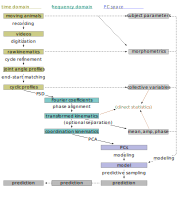
\includegraphics[width=.9\linewidth]{./figures/f8_flowchart.pdf}
\caption{\label{fig:procedure}\textbf{Analysis and Modeling Procedure.} Workflow overview of the preparation, transformation and analysis steps involved in the data analysis on baboon bipedal walking as described in the text, from raw observation (top) to statistical inference and multivariate analysis (bottom). At each point of the procedure, transformation between the domains is possible and quality checks should be performed.}
\end{figure}

\subsection{Data Preparation}
\label{casestudy:dataprep}
After data acquisition is complete and hard drives are filled with videos, the individual stride episodes which were captured on video must be annotated and extracted.
As a good approximation, one can use the conventional touch down timepoints (though lift off or mid stance would work equally well, and the choice may vary within the dataset).

\begin{figure}[p]
\centering
\includegraphics[width=.9\linewidth]{./figures/f4_raw_inspection.pdf}
\caption{\label{fig:raw_inspection}\textbf{Raw Data Inspection.} (A) Plotting a series of stride cycles in the camera reference frame can aid the identification of data discontinuities (visible here in the distal limb markers). The animal is moving from left to right. A stick figure displayed for the last frame facilitates landmark attribution (torso, tail, hind- and forelimb are shown, similar to Fig. \ref{fig:endstart}). (B) Plotting one stride in the moving reference frame of the subject (zoomed in on the limbs) can confirm cyclic/steady state movement.}
\end{figure}


A prerequisite for any meaningful analysis is consistent, complete data.
Data in this case are points of interest, tracked on videos.
There are many tools for video digitization, which are more or less automatic and accurate \citep{MMielke2020,Knoerlein2016,Hedrick2008,Crall2015,Mathis2018,Karashchuk2021,Dunn2021}.
It should be assured that no frames have been involuntarily skipped in the process of tracking, and that there are no discontinuities in the series of point positions.
This can be easily achieved by plotting the time series of digitized points, either in the global reference frame, or in a moving reference associated with the subject (Fig. \ref{fig:raw_inspection}).
After digitization, the aforementioned calculation of Procrustes distances between putative start and end frames (ch. \ref{properties:endstart}) can be used to refine the stride interval and minimize end-start-differences.

With strides identified and data quality assured, collective variables such as duration, speed, clearance, or gait asymmetry can be stored for each stride observed in the dataset.


Next, joint angles can be calculated in a variety of ways.
Their precise definition and direction is arbitrary, yet should be consistent and clearly documented.
Care should be taken that joint angles do not show jumps at any time point of the movement, for example by crossing the \(2\pi\) angular interval border.
Such jumps would lead to a wrong FSD, because that procedure does not natively consider angular value ranges or interval wrapping and thus treats the jump as if it were an actual discontinuity.
The joint angle definition chosen herein, with fully extended limb corresponding to a joint angle of zero, and angles ranging from \(-\pi\) to \(+\pi\), usually avoids such discontinuities.

In the case of two-dimensional joint coordinates, calculation of joint angles is relatively straight forward with an `arctan` formula.
When working in three dimensions, the question is whether sufficient anatomical reference points can be digitized to calculate actual anatomical joint angles.
If not, it must be sufficient to calculate a single angle between the segment vectors, though that does not necessarily correspond to anatomical degrees of freedom.
If instead there are sufficient reference points, multiple rotation axes and angles per joint can be used and integrated just as in a multi-joint analysis (see below).
Note that there have been attempts to directly calculate Fourier coefficients from 3D joint angles, using quaternions \citep{Kenwright2015}, which would be the most elegant solution for this purpose.


After removing end-start-differences as described above (ch. \ref{properties:endstart}), joint angle profiles are plugged into the Fourier equation \eqref{eqn:fourier_coefficients1}, e.g. by using the corresponding programming functions supplemented to this manuscript.
Thereby, joint angle profiles are transformed to the frequency domain.
Though I above emphasized the complex values of the coefficients, they can as well be represented by a one-dimensional array of alternating real- and imaginary parts of the coefficients.
The transformation should be inverted, and original and re-transformed joint angle profiles plotted together, to exclude coding errors and confirm that order was chosen high enough (Figs. \ref{fig:reversibility}, \ref{fig:residuals}).

\begin{figure}[p]
\centering
\includegraphics[width=.9\linewidth]{./figures/f5_reversibility.pdf}
\caption{\label{fig:reversibility}\textbf{Reversibility.} A single joint angle profile, processed forth and back with Fourier Series Decomposition (green, using 9 coefficients) and Principal Component Analysis (orange, using first 5 principal components, after FSD). The residual \(\epsilon\) is the mean of Euclidean distances of all angle measurements over time from their corresponding re-transformation in the time domain. See also Fig. \ref{fig:residuals}.}
\end{figure}

\begin{figure}[p]
\centering
\includegraphics[width=.9\linewidth]{./figures/f6_residuals.pdf}
\caption{\label{fig:residuals}\textbf{Retransformation Residuals,} (A) after performing FSD only with a given order (i.e. number of coefficients, x-axis), (B) after FSD (9 coefficients) and PCA with a given number of retained components. Residuals \(\epsilon\) (y-axis) as defined above. Joint angle profiles of all observed baboon strides are included, the distribution of residuals is indicated by grey ``violins''. Relatively low numbers of coefficients and components are sufficient to get close to the asymptotic accuracy. The absolute residual is joint-dependent (compare hip and knee, for example), an effect which is primarily determined by digitization accuracy and measurement noise. The data point for ``full'' PCA dimension is the reference value with just the FSD.}
\end{figure}

\subsection{Multivariate analysis}
\label{sec:org2c17156}
Each stride processed in the analysis counts as exactly one data point, and so far, data points were considered independently.
The conventional next step is to analyze their relation to each other.

For example, it might be apparent that two or more data points are phase shifted relative to each other: all the characteristic maxima and minima of the joint angle profile would appear later or earlier in the time domain plot.
If one assumed that strides are cyclic, it must be conclude that these phase shifts are due to our arbitrary choice of the start point within the cycle.
Phase differences should therefore be minimized.
However, different joints, when analyzed together, might theoretically give contradicting information on the relative phase shift of different strides.
Obvious solutions are to either choose a reference angle for phase alignment (this might be an angle not otherwise used for analysis: in the baboon test case, I chose the ``total limb'', i.e. the head-hip-toe angle), or to use an amplitude-weighted average phase shift as calculated from all joint angles of interest together.

And just as with phase, there are design choices about whether to keep the other affine components (mean, amplitude) implicit in the multivariate data set, or extract and isolate them for subsequent analysis.


Independent of these choices, the result of the previous steps is a data table consisting of multiple observations (strides, in rows) and variables (Fourier coefficients, in columns).
The observations can be related to their corresponding master data (i.e. subject characteristics, morphology, collective variables, isolated affine components) by a simple stride index.

Such a data structure is eligible for multidimensional analysis methods, and one of the simplest such method is Principal Component Analysis (PCA).
Often, PCA justifies a significant reduction of data dimensionality (i.e. number of data columns), depending on how much variance is concentrated on the first components.
Apart from the residual variance not covered by the retained principal components, PCA is again information preserving and reversible (which should be confirmed, Figs. \ref{fig:reversibility}, \ref{fig:residuals}).
Often, PCA is just used to open the data for subsequent multivariate methods (e.g. factor analysis).


To summarize: in the procedure drafted above, I have extracted and quality checked kinematic measurements from digitizing videos.
Joint angles were calculated and submitted to two transformation procedures: FSD and PCA.
All procedures to this point can be performed without loss of information: any of the resultant data rows could be converted back to an animation of moving points.
Thus, the PCA outcome essentially contains the whole of what was captured by the original kinematic data: the spatiotemporal coordination of the moving body appendages of interest.


\subsection{Statistics and Modeling}
\label{sec:org25fbd32}
Despite the direct link to the raw data, the data table resulting from PCA might seem abstract.
Nevertheless, those values are useful, because they are much more compact than the original two-dimensional time series of varying length.
And this compactness is crucial for statistical testing and modeling, for which computational complexity can be restrictive.


As a proof of concept, I herein briefly present the outcome of one type of analysis approach: probabilistic modeling (to be discussed in all detail in Ch. \ref{cpt:statistics}).
The two major advantages are that (1) probabilistic models capture the variability of the intrinsically variable process of locomotion, (2) such models can be used for extrapolation (out-of-sample prediction).


The usual modeling steps are:
\begin{itemize}
\item data simulation (prior to acquisition; can provide valuable information on required sample size, feasibility, and model structure)
\item model construction
\item (MCMC) sampling
\item model comparison and refinement
\item posterior checks (model ``hygiene'')
\item predictive sampling
\end{itemize}


I applied all these to the baboon data set.
In total, \(40\) stride cycles from \(17\) subject individuals entered the analysis.
I applied a stepwise modeling approach, modeling the PCA-transformed Fourier coefficients (\(\theta\)) generated from a set of joint angles (hip, knee, and ankle) as a function of sex (`male`), age class (`adol`, `inft`), body mass (`cbm`/centered), limb length (`ll`), clearance (`clr`), duty factor (`df`), trunk angle (`trnk`) and speed-related parameters (`str`, from a PCA of stride duration, length, speed and frequency).
\begin{equation}
\begin{split}
 \theta_{i}  \sim &\quad v_{1,i}\cdot\alpha_{i} +
\\ & + v_{male}\cdot\beta_{male,i} + v_{adol}\cdot\beta_{adol,i} + v_{inft}\cdot\beta_{inft,i} + v_{cbm}\cdot\beta_{cbm,i}+ v_{ll}\cdot\beta_{ll,i} +
\\ & + v_{clr}\cdot\beta_{clr,i} + v_{df}\cdot\beta_{df,i} + v_{trnk}\cdot\beta_{trnk,i} + v_{str1}\cdot\beta_{str1,i} + v_{str2}\cdot\beta_{str2,i} +
\\ & + \epsilon_{i}
\end{split}
 \label{eq:jap}
\end{equation}


In the case of the baboon data set, I was able to successfully train this complex model despite limited sample size.
I then confirmed model convergence and ensured that the model is favorable over alternative models with more or less parameters.
The implementation in PyMC (a Pyhton library, \url{https://www.pymc.io}) has the capability of posterior predictive sampling: the trained model can be used to generate an arbitrarily high number of virtual data points, which underly the same variability as the original data.
Most notably, this includes predicting ``out-of-sample'', i.e. parameter combinations which were not directly observed (in this case, male adult baboons were not included in the data, but could be predicted; Fig. \ref{fig:modelprediction}).
Though the model infers abstract PCA values, the much emphasized reversibility of the method enables the computation of joint angle profiles from the predicted values.
For interested readers, all data and documented code for all the steps described above are available online (\url{https://git.sr.ht/\~falk/papio\_fcas}).


\begin{figure}[p]
\centering
\includegraphics[width=.9\linewidth]{./figures/f7_trace_predictions.png}
\caption{\label{fig:modelprediction}\textbf{Posterior Predictive Sampling.} A probabilistic model which is trained on the kinematic data (dark grey lines) is capable of predicting joint angle profiles (colored, thin lines; 1000 predictions per category). This can be extrapolated, for example to unobserved category combinations (here: adult males, which were not part of the dataset). Model design and training are enabled by transformation of the data to a PCA-space of the frequency domain. Joint angle profiles are centered around their mean for visualization; black bar in the lower left plot indicates angular units.}
\end{figure}


This modeling and prediction is complementary to and consistent with the analysis of \citet{Druelle2021}.
A targeted model design could for example serve to infer effects of ageclass, speed, or their interaction, as was done in the original treatment of this data set.
Such research questions can be addressed without transformation to the frequency domain.
However, the point highlighted here is that the frequency domain data retains almost the full kinematic information, and thereby enables assessing a broader range of quantitative analysis questions, and predictive modeling of joint angle profiles and coordination.

\FloatBarrier\clearpage
\section{Summary}
\label{summary}
When reviewing prior attempts to use Fourier-based methods for the analysis of kinematics, a lack of consistency becomes apparent.
Prior studies using the method exist, but hardly reference each other, which indicates independent events of lateral Fourier gene transfer into the population of biologists.
Authors seem to be unaware of the different available methods and how to apply them efficiently.
Some of the choices for application are of little relevance for the outcome of the analysis (e.g. whether to use the sine-cosine, exponential, or phase-amplitude form of Fourier Series), whereas others have severe impact (e.g. choice of order).
I pointed out that Fourier methods do not require a regression algorithm for data conversion, and that often the most appropriate tool in the Fourier toolbox to analyze joint angle profiles is Fourier Series (and not FFT).
Usually, few coefficients are sufficient to capture all relevant kinematic information, and multivariate methods such as PCA are readily available for further dimensionality reduction.
Some properties of joint angle profiles become directly accessible by FSD (affine components), and a mathematically precise phase alignment is possible.

Yet, as demonstrated above, I would argue that the biggest advantage of transforming the data to the frequency domain is that it enables the quantitative analysis of coordination.
Though joint angle profiles could theoretically be resampled and submitted to multivariate analysis directly, this approach would face major technical challenges if sample size is limited, or data points are structurally different, misaligned, or undersampled (all of which is practically always the case in comparative kinematics).
FSD circumvents these problems by providing an elegant, concise representation of the data: a set of relatively few, partially meaningful complex coefficients which can be converted back to the original data.


This availability for quantitative analysis has far reaching potential.
I demonstrated it on a relatively small, but well studied data set of bipedal walking in baboons, and were able to predict stride cycles for a coincidentally unobserved combination of subject attributes.
Using phylogenetic and morphometric bracketing, the same procedure could be applied to infer the locomotion of extinct species, e.g. hominids.
Another potential purpose of this quantitative method is its combination with dynamics, i.e. force and moment measurements:
consider a perturbation analysis, where normal locomotion is interrupted, and a subject can succeed or not in maintaining dynamic balance.
Certainly, success will depend on the specific movement of some limb elements, and quantitative kinematic modeling can highlight which.

I will get back to and extend the use of FSD and the probabilistic modeling approach in the following chapters (Ch. \ref{cpt:statistics}, Ch. \ref{cpt:piglets}).


None of these analysis components are novel.
Fourier Analysis is a standard tool in physics and engineering.
I see equally great potential for the biological sciences, where cyclic phenomena are abundant (genetics, physiology, behavior, \ldots{}).
I suspect that the reason for the limited use of these tools to date is limited accessibility, caused by terminological confusion and the lack of attention for example studies.
I referenced some excellent work that made use of the Fourier theorem \citep{Bernstein1935,Pike2002,Webb2007}, as well as our own attempts to extend the capability of the technique in the context of kinematics \citep{Mielke2019,Mielke2023}.
Thereby, I hope that this review can increase availability of the Fourier method to biological sciences, potentially even beyond the study of locomotor kinematics.




\FloatBarrier\clearpage
\section{Supplements}
\label{appendix}
\subsection{Computer Code to Apply Fourier Series}
\label{appendix:code}
This is an example how the Fourier Series can be implemented in the Python programming language (\nolinkurl{https://python.org}).

Similar implementations for R and Matlab are provided ``ready-to-use'' on the following git repository:

\url{https://git.sr.ht/~falk/fcas_code}



\begin{lstlisting}
def FourierSeriesDecomposition(time, signal, order):
    # calculate the Fourier Series decomposition of a signal,
    # given the sample time array ("time")
    # and a chosen "order" (i.e. highest coefficient returned)
    # returns complex coefficients

    # the period of the signal
    period = numpy.max(time)-numpy.min(time)

    # number of samples taken
    n_samples = len(time)

    # the exponential formula for each coefficient
    SingleCoefficient = lambda t, T, n: numpy.exp(-1j*2*numpy.pi*n*t/T) / (2 if n == 0 else 1)

    # calculate the Fourier Series as a list of coefficients
    fsd = (2/period) * numpy.array([ \
                     numpy.sum(signal*SingleCoefficient(time, period, n)) / n_samples \
                     for n in range(order+1) \
                    ])

    return fsd

\end{lstlisting}

\pagebreak
\begin{lstlisting}
def FourierSeriesRecomposition(coefficients, output_time):
    # reconstruct a signal from its frequency space representation
    # i.e. take coefficients list and return the signal at given output_time points

    # the exponential used in this formula
    FourierSummand = lambda t, T, cn, n: cn*numpy.exp(1j*2*numpy.pi*n*t/T)

    # the fourier function at a single time point
    FourierFunctionT = lambda t, T, coefficients: numpy.sum(numpy.array([ FourierSummand(t, T, cn, n) \
                                                               for n,cn in enumerate(coefficients) \
                                                              ]))

    # the period "T" of the signal
    period = numpy.max(output_time)-numpy.min(output_time)

    # for every point in time, sum up the coefficients
    signal =  period * numpy.array( [FourierFunctionT(t, period, coefficients) \
                                 for t in output_time \
                                 ]))
    return numpy.real(signal)

\end{lstlisting}


\cleartoleftpage
\chapter{Fourier Coefficient Affine Superimposition}\label{cpt:fcas}



\pagebreak
\section{Abstract}
Many phenomena related to motor behaviour in animals are spatially and temporally periodic, making them accessible for transformation to the frequency domain via Fourier Series.
Although this has been applied previously, it had not been noticed that the characteristic arrangement of Fourier coefficients in their complex-valued representation resembles landmarks in geometric morphometrics.
We define a superimposition procedure in the frequency domain which removes affine differences (mean, amplitude, phase) to reveal and compare the shape of periodic kinematic measures.
This procedure is conceptually linked to dynamic similarity, which can thereby be assessed on the level of individual limb elements.
We demonstrate how to make intralimb coordination accessible for large scale, quantitative analyses.
By applying this to a data set from terrestrial ungulates, dominant patterns in forelimb coordination during walking are identified.
This analysis shows that typical strides of these animals differ mostly in how much the limbs are lifted in the presence or absence of obstructive substrate features.
This is shown to be independent of morphological features.
Besides revealing fundamental characteristics of ungulate locomotion, we argue that the suggested method is generally suitable for the large scale quantitative assessment of coordination and dynamics in periodic locomotor phenomena.


%________________________________________________________________________________________
%	Intro
%________________________________________________________________________________________
\pagebreak
\section{Introduction}
A prevalent feature of motor behaviour of animals is temporal and spatial periodicity.
Rhythmic or cyclical recurrent patterns can occur on all scales, from large (e.g. seasonal migration) to small (e.g. neural pattern generators, actin-myosin binding).
Locomotion is one behavioural class which is highly relevant for the organism, and which often shows a considerable degree of recurrence, most prominently during steady-state locomotion.
In consequence, locomotion was one of the first subjects of motor behaviour to be formally studied \citep{Marey1878,Muybridge1893,Braune1904,Bernstein1927a,Bernstein1927b}.
In the study of terrestrial locomotion, limb kinematics (e.g. joint angles) and dynamics (e.g. joint moments, ground reaction forces) represent relevant periodic profiles accessible to comparative analyses.
Groups for comparison can be defined by differences in various attributes, such as for example phylogeny, age and development, physiological background, or pathological status.
Locomotion holds diagnostic potential in all of these: the periodic profiles are ultimately linked to the ecology, ontogeny, and morphology through evolutionary processes, and proximately modified by immediate external and internal constraints \cite[e.g.][]{Barrett2008,McGibbon2003,Mohling2014,Nyakatura2012,Nyakatura2019,Vanhooydonck2014,VandenHole2018}.
\\The analysis of locomotor patterns can be insightful and has been exerted in numerous cases, targeting different levels of detail.
A common tool to quantitatively compare kinematics are spatio-temporal gait parameters, which are summary statistics over limbs, stride cycles, or both \cite[see e.g.][]{Christiansen2002,Biancardi2012}.
The limitation of gait parameters is that they do not resolve differences in intralimb coordination.
Intralimb coordination is a complex phenomenon, which has been difficult to capture in quantitative methods.
In some hallmark studies, the comparative analysis of intralimb coordination has been performed by relatively sparse sampling from large groups, with nevertheless respectable workload \citep{Stoessel2012,Fischer2002,Isler2005}.
Gatesy and Pollard \cite[2011, ][]{Gatesy2011} have attributed the limited quantitative accessibility of coordination to limitations in transferability of kinematic profiles.
According to their theoretical considerations, the temporal change of a joint angle within a limb can hardly be disentangled from morphology, posture, and the interaction with adjacent joints, which makes it hard to transfer observations between groups.
These authors call for novel methods to resolve these dependencies.
We herein present such a method, and exemplify it on a broad sample of terrestrial ungulates.
The backbone of our approach is Fourier Series decomposition (FSD).
Its novelty lies in an attempt to superimpose temporal profiles in a manner analogous to geometric morphometric techniques, i.e. using FSD to extract the ''shape'' of cyclic curves.
\\To extract shapes from such temporal profiles (or any periodic signal in general), one requires data that resembles landmarks, as well as a procedure to superimpose observations.
Profile landmarks can be found by applying Fourier Series.
Fourier Series is a classical method in the study of kinematics \citep{Bernstein1927a,Bernstein1935}, although there are few recent studies exploring it further \citep{vanWeeren1992,Grasso2000,Webb2007}.
Note that Fourier Series is related to, but different from other techniques previously applied in the context of locomotion (namely Fourier Transform and Elliptical Fourier Descriptors, see discussion).
By applying FSD, the signal is decomposed into its harmonics, which describe it in what is called the frequency domain.
The outcome of FSD is usually reported as sine- and cosine coefficients, which through Euler's formula are equivalent to complex exponentials.
As will be illustrated further, this latter representation has some advantages for our purpose.
When plotted in the complex plane, Fourier coefficients have characteristic arrangements, which we find are to an extent analogous to landmarks in geometric morphometrics \citep{Bookstein1991,Kendall1989}.
Furthermore, the \textit{affine} components of a signals become mathematically accessible in the complex plane representation.
Affine components are those that can be scaled linearly without altering the shape of the signal.
In the case of complex Fourier coefficients, those are (i) the mean profile value (i.e. ''y-value'') over time, captured as the zeroth Fourier coefficient, (ii) the amplitude of the harmonics, visible as the distance from the origin of the complex plane, and (iii) the phase, which is related to a (non-trivial) rotation in the complex plane (\textit{cf.} methods, Fig. \ref{fig:workflow}).
These terms are analogous to the parameters of a harmonic oscillation of frequency $f$ over time $t$ of the form ''$y = c_0 + A\cdot sin(2\pi f\cdot t + \phi)$''.
Such an oscillation has the mean $c_0$, amplitude $A$, and the phase $\phi$.
Assume there is a mathematical operation that removes the affine differences between two such oscillations by shifting (i.e. changing $c_0$), scaling (changing $A$), and rotating (changing $\phi$) the complex coefficients in the frequency domain to a standardized arrangement.
This would be a Procrustes procedure which results in a mathematically optimal superimposition (two harmonic oscillations of the same frequency would become identical).
We explore such a superimposition in this study, terming it Fourier Coefficient Affine Superimposition (FCAS, see below).
\\The motivation behind this is the search for a quantitative, comparative measure of coordination of joints along a limb.
For such measurements to be comparable, one should normalize the measures according the the dynamic similarity principle.
Dynamic similarity, in general and in its biological application \cite[\textit{cf.}][]{Alexander1983,Vaughan2005}, is also concerned with the isolation of affine components.
In general, dynamic similarity applies when all spatial dimensions of two mobile systems scale with the same factor (i.e. geometric similarity), the temporal aspects of all involved movements scale with another, again uniform factor (i.e. similar coordination), and therefore all forces are similar except for a uniform third factor.
Scaling the system by such factors represents an affine transformation.
In the specific case of terrestrial locomotion, dynamic similarity allows predictions about kinematics and kinetics of different animals \cite[i.e. about leg phasing, relative stride length, duty factors, forces and power output;][]{Alexander1983}.
In practical application, a common purpose of the dynamic similarity principle is to compare animal locomotion at equal Froude numbers \cite[e.g.][]{SteudelNumbers2006,Holmes2006}.
Perfect dynamic similarity is rarely observed and not expected, but finding the reason for deviations from it can be instructive \cite[e.g.][]{SteudelNumbers2006,Raichlen2013,Kramer2013}.
Such studies are usually concerned with spatio-temporal gait variables.
We attempt to apply the dynamic similarity principle on the level of joint angles, i.e. to measure intralimb coordination, using FCAS as a method to separate affine and non-affine differences in time profiles of joint angles.
\\A classical illustration of the concept of dynamic similarity is the case of terrestrial ungulates \citep{Alexander1983}.
These are a group of mammals that successfully populated an impressive variety of habitats, such as cluttered rain forests, swamps, rugged mountainsides, plain grasslands, and even deserts.
Ungulates have achieved this without fundamental adjustments in the topology of the locomotor apparatus \citep{McMahon1975,Alexander1984}, albeit variation in their limb geometry.
The musculoskeletal layout and posture of ungulates favour movement that is characterized by parasagittal limb excursions \cite[][]{Jenkins1971,Stein1997}.
Therefore, their locomotor characteristics can be adequately approximated by time profiles of two-dimensional joint angles.
Despite this simplification, their enormous diversity makes ungulates a challenging subject for conventional analyses of intralimb coordination.
During steady state locomotion, joint angle profiles are approximately periodic, thus FSD and FCAS can be applied.
We herein use ungulate kinematics as a case study for FCAS.
\\FCAS does not reveal intralimb coordination \textit{per se}.
However, the fact that superimposition operators (and with them affine differences between groups) are transferable to adjacent joints can be exploited \cite[analogous to][]{Mielke2018b}.
More specifically, in this study, we will perform superimposition of elbow joint angle profiles with respect to the carpus joint.
This example application of FCAS yields \textit{relative} angle profiles, which are quantitative measures of intralimb coordination because they contain the combined variance from two joints.
Using the frequency domain representation, the relative profiles become accessible for multivariate analysis.
These ingredients allow us to investigate intralimb coordination in a quantitative comparison of unprecedented phylogenetic scope, overcoming previous limitations \citep{Gatesy2011}.
\\In this study, we focus on the practical application of FCAS and the insights it extracts about ungulate locomotion and evolution.
We supplement a detailed mathematical description (appendices \ref*{apdx:digitization}, \ref*{apdx:fourier}), an extensively commented, open computer code tutorial (supplementary data \ref*{supp:tutorial}), and all data that was generated (supplementary data \ref*{supp:data1}, \ref*{supp:data2}).
We present data of walking gait, densely sampled across terrestrial ungulates (87 of 117 genera).
For this purpose, we digitized freely available video material from online video platforms, as others did before \citep{Biancardi2012,Lees2016}.
Rather than fixing an \textit{a priori} hypothesis, we are interested in extracting major patterns of variation in intralimb coordination in the proximal forelimb of ungulates.
We discuss evidence for deviations from dynamic similarity, and possible reasons.
This provides hypotheses for future, more controlled experimental tests that can likewise benefit from the herein proposed analytical methodology.



\FloatBarrier\pagebreak
%________________________________________________________________________________________
%	Methods
%________________________________________________________________________________________
\section{Materials and Methods}
\subsubsection{Data Acquisition}
The data for this study was acquired from an online video sharing platform (\nolinkurl{youtube.com}).
Genera were searched in Latin, English, or various local languages and search results were scanned for episodes of walking in approximately lateral perspective that did not show signs of \textit{post hoc} manipulation (cutting, etc.).
Slow motion recordings were included if the frame rate was available in the video description.
To exclude confounding variability due to the non-standardized recording circumstances, i.e. to get controlled reference measurements that ensure the validity of the online data, we supplemented high quality recordings of some genera available at our institute or local zoological gardens (34 stride cycles from 11 videos; \textit{Bos}, \textit{Equus}, \textit{Lama}, \textit{Tapirus}).
In total, 388 videos contained candidate episodes and were annotated and cut (i.e. full stride cycles) in ELAN software \cite[Max Planck Institute for Psycholinguistics, Nijmegen;][]{Brugman2004}.
Episodes were selected to have sufficient temporal and spatial quality and correct perspective (movement perpendicular to the view axis).
Videos of juvenile individuals were rarely included, i.e. only in cases where few recordings were available for a genus.
Video cutting was performed in the free video manipulation software ''FFmpeg'' (\nolinkurl{http://ffmpeg.org}).
\\Digitization of the animal movement (Fig. \ref{fig:workflow}A) was done in a custom-written tool using the Open Source Computer Vision Library (''OpenCV'', \nolinkurl{https://opencv.org}) interface for the Python programming language (Python Software Foundation, \nolinkurl{https://www.python.org}).
We manually tracked joint center pixel positions over time, digitizing four joints along the forelimb which was ipsilateral to the camera.
From this data, angles were calculated, various quality checks applied, and it was ensured that the angle profiles (i.e. joint angles over time) were cyclical (for a detailed procedure, see appendix \ref*{apdx:digitization}).
The videos with episodes that passed quality criteria were reviewed to register species, sex, speed, duty factor, and degree of obstruction (see below).
The final material covers 87 of 117 genera (109 of 251 species) of terrestrial ungulates.
556 stride cycles passed strict quality checks, stemming from 217 of the videos (supplementary data table \ref*{supp:data1}).


\subsubsection{Fourier Series Decomposition (FSD) Exposes Affine Signal Components}
We herein study periodic joint angle profiles, but with methods that generally apply to periodic signals.
There are two fundamental ways in which two or multiple signal observations can differ.
One type of differences are those which can be removed by a linear operation (i.e. addition or multiplication of scalars).
Those are the mean, amplitude, and phase, which can be removed by ''y-shifting'', scaling around the mean, and phase-shifting, respectively.
These differences are termed affine differences.
Other affine operations exist (reflection, shear, planar rotation), but they do not apply to time profiles because they disrupt the spatio-temporal integrity of the signal.
Differences that cannot be removed by affine transformations are subsumed as non-affine.
\\In the time domain (plot of the signal value over time, Fig. \ref{fig:workflow}A), the affine differences are intuitively visible, but hard to capture mathematically due to temporal periodicity.
Hence, Fourier Series decomposition (FSD, as defined in appendix \ref*{apdx:fourier}) is applied to the signals we study herein.
This transformation decomposes a signal into a finite sum of its harmonics.
These harmonics are wave functions for which the product of their signal period $T$ (i.e. full cycle recording duration) and frequency $f$ is an integer (e.g. $T = 2.1\ s$, $f = 3/2.1\ Hz$, which is the $n=3^{rd}$ harmonic).
The harmonics are the Fourier coefficients, but instead of the commonly used sine- and cosine representation ($a_{n}$, $b_{n}$), we extract complex exponentials ($c_{n}$; both representations are related through Euler's formula).
Hence, the coefficients herein are complex numbers which, with their real and imaginary part, constitute the frequency domain representation of the signal (Fig. \ref{fig:workflow}B).
\\Complex Fourier coefficients facilitate the extraction of information about affine components of the signal (see appendix \ref*{apdx:fourier}) because rotational operations are conveniently applied with complex exponential factors.
Affine differences translate to the coordinate positions of the coefficients in the complex plane: the zeroth coefficient $c_{0}$ reflects the temporal mean, whereas polar coordinates of the other coefficients  (distance from origin, rotation relative to positive real coordinate axis) map the amplitude and phase of the signal (Fig. \ref{fig:workflow}B).
The transformation has an interesting effect on the temporal sampling.
Take, for example, a signal composed of 20 measurement samples over the cycle.
To phase shift, one could ''roll'' the vector of samples, e.g. appending the first sample at the end.
Intermediate phase-shifts are inaccurate because they require interpolation.
In the frequency domain, the signal becomes independent of temporal samples (\textit{cf.} appendix \ref*{apdx:fourier}), except that sampling gives an upper limit to the number of harmonics that can be extracted.
In consequence, phase information becomes continuous, phase shifting is not restricted to the temporal raster defined by sampling, but no interpolation is required.
Conversely, series decomposition with a finite number of harmonics leads to low pass filtering, hence FSD removes high frequency components from the original signal.
\\An overview of how affine changes affect the signal in time and frequency domain can be found in the online supplements, together with an implementation of FSD (supplementary data \ref*{supp:tutorial}).
It is important to note that all of FSD and the procedures described below are deterministic.
Hence, none of these require a fitting- or optimization algorithm.
In previous studies, it has been quite common to determine Fourier coefficients by approximation \cite[e.g.][]{Alexander1980} or an iterative algorithm \cite[regression, e.g.][]{Hubel2015}.
A deterministic implementation is more efficient and less error prone and should thus be strictly preferred (the space that an optimizer has to traverse is complex due to angular ambiguity; there are inherent phase relationships of coefficients that common samplers ignore).
We also recommend to reconstruct test signals from coefficient values for visual comparison with the original signal to confirm that the decomposition was accurate.



\subsubsection{Fourier Coefficient Affine Superimposition (FCAS) Reveals Signal Shape}
Taking all coefficients derived from the FSD of a signal together is data that is structurally analogous to two-dimensional landmarks.
Hence, methods of geometric morphometrics can be applied \citep{Bookstein1991,Kendall1989,Gower1975,Dryden2016}, in particular Procrustes superimposition, which is a method that removes affine components of the form of an object to reveal its shape.
For the complex Fourier coefficients, it is possible to define standard values for the affine components (i.e. mean of zero, amplitude of one, phase zero) and operators that shift or scale the signal to achieve standardization.
Similarly, it is possible to find, extract, and apply operators that superimpose two signals by removing affine differences (Fig. \ref{fig:workflow}C), which we term FCAS.
In contrast to geometric morphometrics, the rotation is not uniform, but depends on the harmonic number.
Also, the translational component is restricted to $c_{0}$, and all higher coefficients are only affected by rotation and scaling.
These modifications do not hinder the general procedure.
Analogous to the process of Generalized Procrustes Analysis in geometric morphometrics, the superimposition can be applied to find improved averages of signals.
The (non-affine) residual after removal of affine differences is, in analogy to geometric morphometrics, the ''shape'' of the signal, and it is possible to define distance metrics to quantify shape differences (though not relevant for the present study).
\\In case kinematic measures, such as joint angle profiles, are the signals of interest, both affine and non-affine differences can have consequences for the kinetics.
However, only non-affine differences imply different coordination, whereas affine components are merely a change in temporal or spatial scale of the same patterns.
Coordination should be evaluated in context of the limb.
Hence, when regarding multiple joints along the limb, it is crucial to retain the coupling of the limb joints.
For example, when phase aligning carpus joint profiles (reference joint, for reasons discussed below), the same time shift should be applied to other joints of the limb (focal joints, herein the elbow, Fig. \ref{fig:workflow}D).
Similarly, a normalization of the mean and amplitude of the reference joint can be applied to focal joints, which then express relative mean and amplitude.
When applying operators from a carpus joint superimposition to the elbow joint profiles, we term this ''carpal superimposition of the elbow'', and retrieve ''relative elbow profiles''.
This transfer shifts the affine variance from the carpus to the elbow joint.
For example, if in species A the carpus phase is lagging $+0.05$ stride cycles relative to species B, but the elbow phase difference of the two species is $-0.1$ (A before B), then the phase of the relative elbow profile of species A will be $-0.05$ with respect to that of B.
Hence, relative profiles capture intralimb coordination.
They are also represented in the frequency domain, but temporal profiles can be reconstructed at any point for visualization  (margins of Fig. \ref{fig:workflow}C and D).
The Fourier coefficients of relative elbow profiles are subjected to further analysis.
Because we are interested in dynamic temporal changes relative to the mean angles, we remove differences in $c_0$ by subtracting it from the profiles, despite acknowledging that posture or average angle might affect the dynamics.

\subsubsection{Multivariate Analysis}
A variety of multivariate methods exist that could be explored with relative elbow profile Fourier coefficients.
Because our study is introducing a previously unexplored method (FCAS), we restricted post processing to plain Principal Component Analysis (PCA, Fig. \ref{fig:workflow}E).
PCA was applied to the real and imaginary parts of relative elbow FSD coefficients.
By an eigenanalysis of the covariance matrix of the coefficient table, PCA finds orthonormal axes which orient the data in a way that shows the major variation \cite[\textit{cf.}][]{MacLeod2007}.
This was manually implemented in Python, using singular value decomposition (\textsf{numpy.cov}, \textsf{scipy.linalg.eig}).
We apply it to genus averages \citep{Mitteroecker2011} of FSD coefficients of relative elbow profile (i.e. after FCAS with regard to carpus).
\\The component axes are not \textit{per se} biologically meaningful, but can be associated with covariates.
Covariate choice is arbitrary, but depends on the question of interest.
In our case, four classes of covariates which potentially have a relevant connection to intralimb coordination were collected.
In addition to that, we quantified the affine composition of the relative profiles.
The covariate classes are morphology, gait parameters, ecology and phylogeny.
\\First, characteristics of general and musculoskeletal morphology determine locomotor function.
Species- and sex-specific average measures of body length, shoulder height, and body mass were taken from online data repositories \citep{UltimateUngulate,AnimalDiversityWeb}.
For measures on the video, segment lengths were taken from pixel distances of the tracked points, but normalized as indicated below to remove differences in video resolution.
To evaluate lever relations at the critical joints, zeugopodial length (elbow-wrist, normalized to withers-croup distance) and the meta- to zeugopodial length ratio were included.
Under ideal circumstances, segments should measure equal length in every frame.
However, there is uncertainty in the digitization procedure.
In addition, in cases where the fetlock joint was covered by vegetation during ground contact (but not during the swing phase), tracking points were shifted proximally along the limb segment to still be able to capture the (carpus) angle over time.
The framewise $90\%$ quantile value turned out to be robust to episodes when joints were hidden during stance, while being sufficiently close to the true mean segment length (i.e. robust to inadvertent tracking outliers).
\\Second, intralimb coordination potentially covaries with spatio-temporal gait parameters (kinematics).
From the video data, duty factor (ratio of stance- and stride time) and approximate speed (body lengths per second, from back line to reference landmark movement) could be measured.
The exact Froude number was unavailable, since the spatial scale of the videos was unknown.
Furthermore, a proxy for clearance \cite[\textit{cf.}][]{Austin1999} was calculated, i.e. how much the hoof is lifted above the ground during a limb swing.
This required the effective limb extension ($\xi$), defined as follows, from segment ($i$) lengths ($l_{i}$) and their proximal joint angles ($\alpha_{i}$, Fig. \ref{fig:workflow}):

\begin{equation*}
\xi = \sum\limits_{i} l_{i} \cdot \cos{\alpha_{i}}
\end{equation*}

We define clearance as the quotient of the $5\%$ and $95\%$ quantiles of $\xi$ over time (which quantifies limb flexion ratio), subtracted from one.

\begin{equation*}
\text{clearance} := 1 - \frac{\xi_{5\%}}{\xi_{95\%}}
\end{equation*}

Again, quantile values were used because the extremal values would be at the far tail of the Gaussian noise associated with point tracking.
\\The third group of covariates are ecological parameters.
In particular, we were interested in the species habitat and the momentary environment at video recording.
We followed the method of Stankowich and Caro (2009) to quantify habitat openness \citep{Caro2004,Stankowich2009}.
Web resources indicated multiple habitat preferences for most species, in which case an uninformed average of the openness values was taken.
The momentary openness, or its inverse (''degree of obstruction''), was determined by noting how far substrate clutter reached up the supporting limbs of the animal in each video.
Values ranged from $0$ (hoof visible) to $0.9$ (limb visible to just below the carpus joint, see supplementary data table \ref*{supp:data1}).
\\The fourth covariate was phylogeny \cite[see appendix \ref{apdx:phylosig} and Fig. \ref*{fig:phylogeny};][]{Zurano2019,Adams2014}.
\smallskip\\Except for phylogeny (which is directly estimated), associations of covariate genus averages and principal component scores of genus means \citep{Mitteroecker2011} were assessed by calculating Pearson correlation (Python: \textsf{scipy.stats.pearsonr}).
Within-group variability was high and observation count heterogeneous across groups, and we applied many correlation tests.
Hence, we only deemed associations with $p<10^{-2}$ relevant.
\\It can be instructive to quantify how much each of the affine differences contributes to the overall relative elbow trace difference.
Therefore, the affine operations that would align the genera averages with their global average were computed.
We report the correlation of these affine differences to the PC axes, as well as the residual shape difference that would remain after their removal.



\FloatBarrier\pagebreak
%________________________________________________________________________________________
%	Results
%________________________________________________________________________________________
\section{Results}
\subsection{Superimposition of Joint Angle Profiles Improves Profile Averaging}

To demonstrate the effect of FCAS, we applied the method to our most extensively sampled genera (\textit{Equus}, \textit{Lama}, and \textit{Giraffa}; Fig. \ref{fig:superimposition}).
Raw data (''video aligned'') was manually aligned for the video frame of limb touch down for comparison with the computational alignment.
Although this was done at maximum possible accuracy ($\pm 1\ frame$), averages revealed no clear similarities or differences between the three genera.
Standard deviation ranges were comparatively high and averages could potentially suffer from incorrect phase relations (analogous to destructive interference) or artificial amplitude weight (because at a fixed time point, particularly high absolute values might attract the average).
FCAS was subsequently performed with regard to carpus joint profiles (Fig. \ref{fig:superimposition}, ''superimposed'', ''[c]'' for carpus joint).
Afterwards, carpus profiles were practically identical for the three example genera.
Elbow joint profiles (''[e]'' in Fig. \ref{fig:superimposition}) were kept in synchronization and amplitude relation with the carpus profiles and were therefore processed with the same operators, resulting in relative profiles (see methods).
Note that no additional superimposition or alignment was performed, except for centering the profiles around their mean.
Relative elbow profiles revealed a precise similarity of lamas and giraffes with regard to coordination of the two joints, which was not obvious from the ''video aligned'' traces.
In contrast, equid intralimb coordination indicated a higher amplitude and a slight phase delay at the elbow (triangle marker, Fig. \ref{fig:superimposition}), relative to carpus joint.
Thus, equids turn out to be more distinct from the other groups than was visible prior to FCAS.
\\This example indicates the increased accuracy of joint profile averaging after FCAS, even in the presence of noise.

\subsection{Patterns of Variation of Ungulate Intralimb Coordination}

We aim to extract the most prevalent patterns of variation in ungulate intralimb coordination.
Therefore, we used the same superimposition procedure as above to generate genus averages for the full data set.
Average angle profiles of all joints and genera (\textit{cf.} Fig. \ref*{fig:phylogeny} for overview of phylogeny) were  then superimposed with reference to the global mean carpus (carpal superimposition).
Thereafter, a PCA was performed on the Fourier coefficients of genus average relative elbow profiles (Fig. \ref{fig:pca}).
The first component axis captured $37\%$ of the variance, and the next three principal components further $49\%$ (PC2: $27\%$, PC3: $12\%$, PC4: $10\%$).
Together, they span the ungulate elbow ''coordination space''.
In that space, bovids and cervids, which contributed the majority of genera, dominate the central region.
On PC1, we observed a spread of bovids from {Bovinae} to {Caprinae}.
For cervids, who spanned almost the same range on that axis, there was no clear grouping.
Tragulids were found on higher values of PC1.
A useful aspect of PCA is the possibility to reconstruct hypothetical joint angle profiles at arbitrary points of coordination space (black line plots at the lower figure margin, Fig. \ref{fig:pca}, no. 1-4).
From these, it can be seen that the major difference is how much the relative angle changes during ground contact.
Ground contact (stance phase) begins with limb touch down (left end of the line plot), continues for approximately the first half of the line, and is followed by a shorter swing phase.
At low values of PC1, the relative elbow profiles (no. 1) are ''sawtooth-like'' curves with steeply sloped, increasing stance phase angles.
These profiles are characterized by two periods of relatively constant slope, one rising (elbow extension, during stance) and one falling (flexion, during swing).
The slope of these curves changes in between these periods, which approximately coincides with hoof touch down and lift off.
Extension of the elbow joint happens during ground contact, hence we call this type of profile ''grounded elbow extension''.
In contrast to that, elbow angles that cluster on high PC1 values (no. 2) only change during the swing phase (brief period of consecutive down- and upward slope), whereas they are close to zero during stance, indicating a straightened joint.
Elbow extension is almost absent during stance (approximately horizontal curve), and after swing-related flexion, an extension follows immediately while still in the swing phase (''swinging extension'' type profile).
\\PC2 separated a cluster of Rhinocerotidae and Suina (upper left) from the rest.
Their relative elbow swings (represented by no. 4) were of lower relative amplitude and slightly phase delayed than those of groups on the opposite end of PC2 (reconstruction no. 3).
\\Standard deviations within groups were high (not shown; approx. $\pm 0.02$ for \textit{Giraffa} on PC1) and sample size was low for many groups.
However, overall group and observation counts were sufficient to describe population effects.
In addition to the shape reconstruction, the direct comparison of geometrically or phylogenetically related genera along the major axes could confirm the mentioned trends (i.e. stance phase slope, relative peak timing and amplitude; Fig. \ref*{fig:examples}).
This further supported the observations from PCA reconstruction.
\\In summary, the PCA, profile reconstruction, and taxa comparison allow the identification and visualization of major differences in intralimb coordination among the studied groups.


\subsection{Covariates of Intralimb Coordination}


To evaluate possible explanations for the variation along principal component axes, we computed Pearson correlation of the components with various morphological, kinematic, and ecological factors, considering effects with $p<0.01$ to be relevant (Tab. \ref{tab:correlations}).
We also split the joint profile shape after superimposition into (non-)affine components, and quantified which of these affine changes were associated with the PCs or whether the shape (''residual'') was affected (Tab. \ref{tab:correlations}, ''[A]'' category).
These values quantitatively characterized the profile reconstructions from the PCA (Fig. \ref{fig:pca}) and were consistent with the findings reported above.
\\Of the first four component axes, PC1 showed the strongest correlation with clearance ($r = 0.49,\ p < 10^{-5}$) and degree of obstruction ($r = 0.33,\ p < 10^{-2}$).
Comparatively smaller taxa (i.e. lower body mass) tended to appear on higher PC1 values ($r = -0.34,\ p < 10^{-2}$).
PC2 was associated with limb morphology, particularly lever relations (ratio of meta- to zeugopodial length, $r = -0.51,\ p < 10^{-6}$; normalized elbow-wrist segment length, $r = -0.46,\ p < 10^{-4}$), and with duty factor ($r = 0.4,\ p < 10^{-3}$).
PC3 scales with habitat and multiple aspects of size, whereas PC4 captured non-affine shape differences (visible in that it correlated to ''residual'').
\\Hence, by the use of simple correlation, it is possible to associate the variational components identified by PCA with meaningful extrinsic (e.g. ecology) and intrinsic (e.g. morphology) covariates.



\FloatBarrier\pagebreak
%________________________________________________________________________________________
%	Discussion
%________________________________________________________________________________________
\section{Discussion}
In this study, we demonstrated how an application of Fourier theory can be used to extract non-affine differences in joint angle profiles, thereby enabling their mathematically accurate superimposition (FCAS).
The new method has to be classified with relation to existing tools.
As an example of FCAS, we analyze intralimb coordination on a large scale, involving the majority of terrestrial ungulate genera, which has not been possible previously.
The kinematic data from the proximal forelimb of ungulates reveals systematic patterns of variation in intralimb coordination.
These can be linked to extrinsic and intrinsic covariates, thereby proposing hypotheses for specific tests of dynamic similarity at the joint level.


\subsection{Quantifying Intralimb Coordination with FCAS}
Conventional kinematic analysis of intralimb coordination involves visual inspection of angle plots in space and time \citep{Irschick1999,Fischer2002,Stoessel2012,Schmidt2008,Day2007,Polk2002,Nyakatura2010}.
Angle values for statistical evaluation are extracted at fixed ''timemarks'' in the stride cycle.
Taken together, these sampled angles allow for coarse assessment of intralimb coordination, but they potentially sacrifice information.
Timemarks are reference points of putative biological meaning, and it is possible to use them for temporal alignment \cite[e.g.][]{HsiaoWecksler2010}.
However, the number and choice of timemarks involves some critical design decisions.
When for example superimposing only based on limb touch down, the alignment is insensitive to differences in hoof placement trajectories before and after that time point.
The hoof can reach the ground at a flat angle with smooth horizontal deceleration.
But the impact can also be vertical, following a more or less brief period where the hoof hovers above the substrate before being placed.
The end of hoof forwards movement might provide a more homologous timemark, but it might still be that the two cases differ fundamentally in the underlying dynamics at that particular episode of the stride cycle.
FCAS represents a mathematically optimal superimposition that equally incorporates all the information contained in the profiles.
The advantage of this strategy is its independence from selected points, and instead the sensitivity to the joint angle trajectory over the whole stride cycle.
Working in the frequency domain also has the advantage of providing a manageable feature vector for multivariate analysis or classification via machine learning.
Fourier Series requires periodic signals to work upon.
As we argued initially, this requirement is often met in the study of locomotion, in which case a transformation to the frequency domain opens up new ways of analyzing the data.
\\The direct application of Fourier Series \citep{Fourier1822,Gray1995,Bracewell2000} is not novel in the context of kinematics \cite[e.g.][]{Bernstein1935,Webb2007,Wheat2006}.
Note that Fourier Series is related to Fourier Transform \cite[cf.][]{Bracewell2000,Robertson2018}: it is also a transformation, but considers only the reduced frequency domain constituted by harmonic frequencies.
Because the interrelation of segments is of interest, Fourier methods have previously been applied to cyclogram curves.
Cyclograms, or phase portraits, are a direct, two- or three-dimensional visualization of segmental coupling \citep{Bernstein1934,Goswami1998,DAout2002}.
Several quantitative descriptors of cyclograms exists.
Elliptic Fourier Descriptors \citep{Kuhl1982,Wheat2006} are an application of Fourier Series to two-dimensional phase portraits.
This technique is abundant in the study of intralimb coordination \cite[e.g.][]{Polk2008,HsiaoWecksler2010,Rosengren2009}, but influenced by variance in reference point determination.
Although affine-invariant outline descriptors exist \cite[e.g.][]{Arbter1990}, we are not aware of an attempt to apply those to kinematic data.
Planar covariation \citep{Borghese1996,Hallemans2009,Ogihara2014} originated in the pursuit of unifying, general features of gaits, and finds high covariation values by design \cite[choice of segment angles, common temporal swing/stance structure for these, use of PCA;][]{Hicheur2006,Ivanenko2008}.
In contrast, we seek a method to highlight differences across taxa.
Another method that has found application in the analysis of human locomotion is continuous relative phase \cite[CRP, \textit{cf.}][]{Lamb2014}.
This method calculates the difference in instantaneous phases of two signals (using phase portrait plots or the Hilbert transform).
CRP requires removal (normalization) of differences in mean angle and amplitude, whereas our method retains the other affine components.
By intentionally phase-shifting random test signals (not shown), we found that both the relative phase from CRP (averaged over a stride cycle) and the FCAS phase difference as introduced herein (appendix \ref*{apdx:fourier}, Eq. \ref*{eqn:affines_phase}) accurately recover the shift.
However, the methods do not yield identical results when other aspects of the signal are manipulated (which in general complicates the definition of a signal phase).
It is thus possible that Hilbert transform and CRP offer alternatives for phase determination.
Because ungulate joint angle profiles are sufficiently homogeneous, we expect general agreement between the methods for the test case presented herein.
\\All the mentioned related methods have originally been applied to phase plots and cyclograms.
Our approach initially goes one step back, to the transformation of individual time profiles of joint angles.
FSD preserves their shape information, and no \textit{a priori} definition of temporal reference points is required (we herein performed the conventional limb touch down alignment, prior to FCAS, only for comparison).
To generate measures of coordination, one has to combine variance from multiple mobile elements (joints or segments) by aligning with regard to one of them while keeping the intralimb coupling intact.
We exploit the empirically observed uniformity of carpus joint profiles, and use this joint as reference, which is motivated by mathematical convenience.
Although superimposition based on the elbow joint might be biologically more meaningful (for example with regard to a proximo-distal sequence of neural control), it would be a less suitable reference because profiles might be topologically heterogeneous (see below).
Transferring the affine components from references to adjacent, focal joints results in relative angle profiles, which are optimally synchronized (phase) and depict the relative amplitude (scale) and differential mean angle.
If mean angles are not of interest, profiles can optionally be centered.
We argue that this way of superimposition results in measures that overcome the theoretical limitations in transferability of angular parameters \citep{Gatesy2011}: (i) posture can be removed by centering relative profiles; (ii) adjacent angles are combined; (iii) morphology, i.e. segment lengths, can be correlated \textit{ex post} as shown, or could even be multiplied in (effective segment length $l\cdot cos\left(\alpha\right)$; not explored).
\\FCAS crucially depends on reference and focal joints, but is not limited in the choice (or number) of these.
Also, it is not limited to a single limb or to phylogenetic comparisons (for example, pseudo-cyclic episodes during gait transition could be compared) and it could be generalized to three-dimensional measurements.
FCAS results in a mathematically optimal alignment, and is robust against low video frame rate due to the filtering properties of the Fourier Series with a finite number of coefficients.
The capacity of a one-dimensional FSD to remove affine components in the frequency domain has not been emphasized in previous work.
The delay theorem, from which we derive a formula that defines a zero phase (see appendix \ref*{apdx:fourier}, Eq. \ref*{eqn:affines_phase}), is of particular interest.
FCAS is not limited to kinematics, and could potentially be applied to a broad variety of other periodic measurements, such as ground reaction force profiles.


\subsection{Dynamic Dissimilarities in Terrestrial Ungulate Intralimb Coordination}
The purpose of the PCA step in the present analysis is to orient the multivariate data so that maximum variation is revealed.
Variation in this case means dissimilarity.
It is herein applied to relative elbow profiles.
These combine information from carpus and elbow, but the carpus only contributes affine changes (Tab. \ref{tab:correlations}, category [A], ''amplitude'' and ''phase'').
Non-affine variation (Tab. \ref{tab:correlations}, category [A], ''residual'') will stem exclusively from the elbow.
Hence, relative elbow profiles in our case show elbow profiles that are centered, normalized and time-aligned relative to the carpus profiles.
The change of one joint angle relative to another is the most basic measure of intralimb coordination.
From these measures, PCA extracts the ''coordination space'' of the relative elbow joint profiles (Fig. \ref{fig:pca}).
The method also allows to reconstruct hypothetical profiles at arbitrary points in that space.
Overall, the group differences might seem subtle at visual inspection, attributing to the fact that ''bauplan'' and movement mode are homogeneous in the data set.
However, even subtle changes in the coordination of the proximal limb have a considerable lever towards the ground contact point.
Also, the reconstructed profiles are derived quantitatively, incorporating a lot of information.
Hence, they are a sharp image of the most pronounced statistical differences that remain after the removal of affine parts of background variance.
Likewise, dynamic similarity (as usually applied to spatio-temporal gait parameters) refers to similarity in non-affine dynamic measures.
This conceptual link indicates that FCAS enables the direct comparison of dynamic differences in the coordination of large data sets of animals.
For the present measurements of walking ungulates, PCA of FSD coefficients of relative elbow joint angle profiles revealed variation associated with several factors.
One of them could be phylogenetic signal, which we found to be less relevant (appendix \ref*{apdx:phylosig}).
\smallskip\\The most prominent effect revealed by the PCA (PC1, $37\%$ of variance) was related to clearance.
Clearance quantifies how much the animal lifts the foot from the ground during swing phase \citep{Austin1999,MacLellan2010,Perrot2011}.
The component axis was also correlated with animal body mass and momentary degree of obstruction (i.e. how free the path of the animal is), but independent of morphology.
Classical gait characteristics (duty factor, symmetry, i.e. inter-limb coordination) doubtlessly classify all included strides as ''walk'' \citep{Hildebrand1989}, but do not consider intralimb coordination or clearance.
Because all observations are ''walk'', and because no change in duty factor was detected (Tab. \ref{tab:correlations}), the timing of stride- and stance phase is uniform along PC1.
However, the temporal pattern of the net joint moments at a limb joint (i.e. the net result of the moments generated by muscles crossing the joint) will likely differ among the profile types as the movements patterns throughout the cycle differ.
For example, the ungulate elbow in the swinging extension type of relative joint profiles (Fig. \ref{fig:pca}, no. 2) is commonly held stiff during the period of ground contact (constant joint angle value), but quickly flexed and extended during forwards swing.
It thereby resembles the common pattern of the ungulate carpus joint (see Fig. \ref{fig:superimposition}).
In contrast, the elbow joint oscillation of grounded extension type profiles is distributed across the whole stride cycle.
This suggests either that the elbow can be a pivot point of limb movement, in which case more proximal elements could be fixed passively (see below), or that the elbow contributes to limb compliance during stance to minimize vertical oscillation of the center of mass \cite[\textit{cf.}][]{Geyer2006}.
Animals commonly use the grounded extension profiles on obstruction-free substrate, whereas the swinging extension could be interpreted as an alternative mode of walking that animals use on cluttered terrain.
\\The elbow profile modes have different implications for the energetic demands of the locomotor behaviour.
Energetics are affected by the substrate that an animal frequently encounters.
Grounded elbow extension implies non-zero angular velocity at the elbow during all of the stride cycle.
If, as discussed above, more proximal elements are mostly fixed, this would lead to an effective shortening of the part of the limb which is mobile.
This is consistent with evidence of stabilizing modification of the shoulder of equids \cite[][]{Hermanson1992}.
Conversely, muscle arrangement in tapirs, which usually exert higher clearance than horses, shows adjustments that favour shoulder motion \citep{MacLaren2016}.
The effective limb shortening, together with the passive pendulum dynamics of the distal elements on unobstructed ground, would reduce energy expenditure.
In contrast, the brief flexion-extension period in swinging flexion appears to require more energy per stride (quicker angular acceleration in opposing directions, longer effective limb, higher clearance).
At the same time, because collision with substrate features is avoided, this behaviour reduces collisional energy loss \cite[i.e. loss from collision with superficial vegetation or rubble, which has to be distinguished from the collisional models in][]{Ruina2005}.
Negotiation of a substrate with inflexible obstruction might even be impossible without lifting the feet (which is not the general case we observed).
Hence, both profile types can be energetically favourable, depending on the circumstances.
\\This suggests questions of whether and how animals adjust their coordination.
At least some species seem to be able to use elbow profiles with both the grounded- and swinging extension.
This would mean that animals retain full capacity to immediately alter their locomotor mode according to momentary features of the substrate (hypothesis $h0$), though we cannot resolve whether modes are used bimodally or whether intermediate patterns are frequent.
In contradiction with $h0$, we observe distinct groups (e.g. \textit{Alces}, some \textit{Tapirus} species) that seem to walk with exaggerated clearance even on free, solid and featureless substrate.
The apparent continuum along PC1 might therefore be an artifact of averaging strides across genera.
This would imply a certain degree of plasticity, i.e. reduced behavioural flexibility, in consequence of adaptation to their preferred habitat ($h1$).
If $h1$ turns out to be more plausible, it could be tested whether morphology coevolved to reduce hoof-lift energy consumption in genera which show a bias towards compliant limb movement.
If experiments confirm plasticity in locomotor behaviour, it might act at different time scales (ontogenetic: $h1a$, or evolutionary: $h1b$).
Our crude averaging quantification of habitat openness has limited decisive value in this case, also because the original classification focuses on canopy level characteristics \citep{Stankowich2009}.
Uncontrolled variation and sample size within the present data set prohibits an in-depth analysis.
Previous studies found contradicting evidence on whether and how locomotion is influenced by habitat \cite[][]{Stoessel2012,Fuller2011,Arnold1983,Schulte2004,Druelle2019}.
These studies did not superimpose profiles for averaging, except for the conventional alignment to limb touch down.
Measurements under more controlled experimental circumstances are required to settle the case between ''walking mode flexibility'' or ''(adaptive) plasticity''.
\smallskip\\The second-largest share of variation in the present data set (PC2, $27\%$ of variance, Fig. \ref{fig:pca}) shows strong association with morphological indicators.
Both the length of the zeugopodial (elbow-wrist, normalized for shoulder-pelvic length; Tab. \ref{tab:correlations}) and the lever relations at the carpus (metapodial/zeugopodial length ratio) decrease with increasing PC2 values.
In accordance with this, the component spans a morphological range from marsh deer (\textit{Blastocerus}) and pronghorn (\textit{Antilocapra}) to peccaries (Tayassuidae) and rhinos (Rhinocerotidae; see also Fig. \ref*{fig:more_pca}).
The geometric dissimilarity along the axis is a case of dynamic dissimilarity, but in addition to that our analysis provides insight on how the elbow-carpus interaction is affected.
Genera at low PC2 values have long limbs and comparatively long distal segments.
This correlates with a higher relative amplitude at the elbow and conversely less angular movement at the carpus, as well as a comparatively shorter stance phase (without notable overall increase in clearance).
In contrast, groups at high PC2 are stout and have comparatively shorter metacarpals, which correlates with slightly earlier and quicker swing.
This lays out a path for future research to evaluate how the angular excursions and the morphological disparity together can be captured by different spring-pendulum models, how they translate to ground reaction force, and what effect this would have on joint moments.





\FloatBarrier\pagebreak
%________________________________________________________________________________________
%	Conclusion
%________________________________________________________________________________________
\section{Conclusion}
Locomotion is costly, responsible for at least $20\%$ (but usually much more) of the energy expenditure of animals \citep{Rezende2009,Girard2001}.
It has long been appreciated that this behavioural class and associated traits must be optimized with regard to the capacities and condition of the animal \citep{Hoyt1981,Reilly2007}.
One reason that optimization is so efficient in locomotion is its high degree of recurrence, which amplifies the effect of ontogenetic and evolutionary adjustments.
Many of the processes involved in locomotion are periodic, and Fourier methods become applicable.
This opens up a variety of analysis paths and can even link kinematics and geometric morphometrics, as we explored in this study.
Our findings on terrestrial ungulates reiterate the requirement to consider habitat structure and substrate as confounding factors \cite[\textit{cf.}][]{Johnson2002,Lejeune1998,Shepard2013}, although it remains to be explored to what degree animals adapt or react to it.
The data presented herein confirms that habitat features and morphology are the dominant determinants of elbow-carpus coordination in terrestrial ungulates.
The moderate magnitude of this variation emphasizes how strongly conserved and optimized ungulate coordination actually is at the joints we investigated, despite the enormous variety of habitats and substrates that these animals encounter.
Our findings from a broad overview of the clade form the basis for hypotheses that can stimulate future research.
It might seem a trivial finding that animals lift their feet more when the path is obstructed.
However, to our knowledge, FCAS is the first method that can confirm this on a large scale because it yields quantitative measures of dynamic similarity on the level of intralimb coordination.


\FloatBarrier\pagebreak
%________________________________________________________________________________________
%	Figures
%________________________________________________________________________________________
\section{Figures And Tables}
\begin{figure}[!ht]
\begin{center}
%\includegraphics[width = 16cm]{fig1_flowchart.pdf}
\end{center}
\caption{\textbf{Analysis work flow, schematic. }
\textbf{A} Video material of walking ungulates is digitized by tracking trace marks (shoulder, elbow, carpus and fetlock joints; see supplementary movie \ref*{supp:movie1}) over a stride cycle, and joint angle profiles are computed (angle defined zero at fully extended limb, positive direction indicated by arrows). Thin black lines are the original measurement, whereas blue lines show the same profile, filtered by FSD with $7$ components.
\textbf{B} Fourier Series decomposition and synthesis allows transformation of temporally periodic angle profiles back and forth between time domain and frequency domain. The zeroth Fourier coefficient ($c_{0}$, lower bar plot) corresponds to the temporal average of the angle profile (i.e. mean angle). The higher coefficients ($c_{n>0}$) can be plotted in the complex plane ($\Re, \Im$); line connections are only for visualization. Coefficients $i$ of joints $j$ have phases ($\phi_{ji}$) and amplitudes ($A_{ji}$), as indicated in gray for $c_{1}$ of the elbow. Average phase and amplitude of the angle profile can be derived (for example $\phi_{c}$, $A_{c}$ for carpus). Mean angle, amplitude, and phase are the affine components of the signal.
\textbf{C} Multiple groups are compared, in this case ungulate genera (\textit{Lama}, \textit{Giraffa}, and \textit{Equus}; coloured in blue, yellow, and brown respectively). By quantifying how they differ in affine components, operators can be extracted ($d\phi$, $dA$, $dc_{0}$). This is facilitated by the transformation to the frequency domain, but a synthesis of time domain traces (line plots on the left and right margin) is always possible.
 \textbf{D} Affine operators are applied to superimpose the joint angle profiles. Superimposition operations from the carpus (reference joint) are applied to the carpus itself, but also transferred to the elbow (focal joint).
\textbf{E} (inset) Fourier coefficients of carpus-superimposed elbow joint profiles are available for multivariate analyses, such as PCA.
  }
\label{fig:workflow}
\end{figure}


\begin{figure}[!ht]%[tbhp]
\centering
%\includegraphics[width=.8\linewidth]{fig2_alignment.pdf}
\caption{\textbf{Superimposition can improve joint angle profile averaging.}
Mean joint angle profiles of different forelimb joints ($[e]$: elbow, $[c]$: carpus joint) for the genera \textit{Equus} (brown, $\triangledown$), \textit{Lama} (blue, $\square$), and \textit{Giraffa} (yellow, $\circ$). These examples were chosen for their high sample size (more examples in Fig. \ref*{fig:examples}). See methods and supplementary tutorial \ref*{supp:tutorial} for nomenclature and definition of FCAS.
\textbf{Upper row}: input data (''video aligned''). \textbf{Lower row}: after carpal superimposition using FCAS.
\textbf{A} Forelimb joint angle profiles ($\alpha$) over time ($t$, stride cycle period $T$), centered around their temporal averages (gray horizontal axes) to emphasize temporal differences. Thick lines are genus averages for elbow (solid line) and carpus (dashed line) angles. Thin dotted lines indicate $\pm$standard deviation range of individual observations. Scale bar $22.5^{\circ}$, time axis $T$.
\textbf{B} Mean (bars) and standard deviation (whiskers) of the joint angle temporal averages ($c_0$) per genus. This indicates the actual $y$-offset that was removed for visualization in (A) and (C). Angle values are to scale with (A).
\textbf{C} The same angle profiles as in (A), but converted to the frequency domain via FSD. Whiskers indicate standard deviation. }
\label{fig:superimposition}
\end{figure}



\begin{figure}[!hb]
%\includegraphics[width = 16cm]{fig3_pca.pdf}
\caption{\textbf{Bivariate plot of the Principal Component Analysis of elbow-carpus coordination visualizes a slice of the ungulate ''coordination space''. }
The PCA is based on the genus average Fourier coefficients of relative elbow profiles after carpal superimposition.
Gray grid lines on the biplot indicate the ($0.1$, $0.9$) quantiles of all observations; reconstructions were done on their intersections.
Outset line plots on the margins represent these reconstructed angular profiles (black) at the quantile values for each component axis, relative to the reconstructed mean (gray).
Their labels (circled numbers no. 1-4) are for reference in the text.
Annotations on the plot mark the examples used in Figures \ref{fig:superimposition} and \ref*{fig:examples}.
See Fig. \ref*{fig:more_pca} for further components and complete labeling of taxa.
 }
\label{fig:pca}
\end{figure}



\begin{table}[!ht]%[tbhp]
\centering
\caption{ \textbf{Correlations of [M]orphological, [K]inematic, [E]cological and [A]ffine covariates} (see methods) with the major axes of the PCA (Figs. \ref{fig:pca}, \ref*{fig:more_pca}). Note that affine covariates are components of the angle profiles. }
\begin{tabular}{l @{$\quad$} cc @{$\quad$} cc @{$\quad$} cc @{$\quad$} cc}
\toprule
{} & \multicolumn{2}{c}{\underline{\textbf{PC1}}} & \multicolumn{2}{c}{\underline{\textbf{PC2}}} & \multicolumn{2}{c}{\underline{\textbf{PC3}}} & \multicolumn{2}{c}{\underline{\textbf{PC4}}} \\
{\textbf{covariate}} &                 $r_{xy}$ &              $p <\cdot$ &                 $r_{xy}$ &              $p <\cdot$ &                 $r_{xy}$ &              $p <\cdot$ &                 $r_{xy}$ &              $p <\cdot$ \\
\midrule
\textbf{[M] body length      } &                    -0.24 &  $10^{-1}$ &                    -0.17 &   $10^{0}$ &                    -0.31 &      $\mathbf{10^{-2}}$ &                    -0.11 &   $10^{0}$ \\
\textbf{[M] shoulder height  } &                    -0.19 &  $10^{-1}$ &                    -0.22 &  $10^{-1}$ &                    -0.33 &      $\mathbf{10^{-2}}$ &                    -0.11 &   $10^{0}$ \\
\textbf{[M] log(body mass)   } &                    -0.34 &      $\mathbf{10^{-2}}$ &                    -0.19 &  $10^{-1}$ &                    -0.28 &      $\mathbf{10^{-2}}$ &                    -0.11 &   $10^{0}$ \\
\textbf{[M] elbow-wrist      } &                     0.05 &   $10^{0}$ &                    -0.46 &      $\mathbf{10^{-4}}$ &                    -0.24 &  $10^{-1}$ &                     0.05 &   $10^{0}$ \\
\textbf{[M] meta-/zeugopodial} &                     0.08 &   $10^{0}$ &                    -0.51 &      $\mathbf{10^{-6}}$ &                     0.01 &   $10^{0}$ &                     0.16 &   $10^{0}$ \\
\midrule\textbf{[K] approx. speed    } &                     0.06 &   $10^{0}$ &                     0.11 &   $10^{0}$ &                     0.12 &   $10^{0}$ &                     0.15 &   $10^{0}$ \\
\textbf{[K] duty factor      } &                     0.16 &   $10^{0}$ &                     0.40 &      $\mathbf{10^{-3}}$ &                     0.19 &  $10^{-1}$ &                    -0.16 &   $10^{0}$ \\
\textbf{[K] clearance        } &                     0.49 &      $\mathbf{10^{-5}}$ &                    -0.02 &   $10^{0}$ &                     0.14 &   $10^{0}$ &                    -0.27 &  $10^{-1}$ \\
\midrule\textbf{[E] habitat          } &                    -0.09 &   $10^{0}$ &                    -0.15 &   $10^{0}$ &                    -0.29 &      $\mathbf{10^{-2}}$ &                    -0.06 &   $10^{0}$ \\
\textbf{[E] d.o.obstruction  } &                     0.33 &      $\mathbf{10^{-2}}$ &                    -0.20 &  $10^{-1}$ &                     0.10 &   $10^{0}$ &                    -0.06 &   $10^{0}$ \\
\midrule\textbf{[A] amplitude        } &                     0.12 &   $10^{0}$ &                     0.47 &      $\mathbf{10^{-5}}$ &                    -0.70 &     $\mathbf{10^{-12}}$ &                    -0.08 &   $10^{0}$ \\
\textbf{[A] phase            } &                     0.47 &      $\mathbf{10^{-5}}$ &                    -0.51 &      $\mathbf{10^{-6}}$ &                    -0.36 &      $\mathbf{10^{-3}}$ &                     0.13 &   $10^{0}$ \\
\textbf{[A] residual         } &                     0.67 &     $\mathbf{10^{-11}}$ &                     0.17 &   $10^{0}$ &                     0.15 &   $10^{0}$ &                     0.36 &      $\mathbf{10^{-3}}$ \\
\bottomrule
\end{tabular}\bigskip
\begin{flushleft}
$r_{xy}$: Pearson correlation coefficient, \nolinebreak{''$p < \cdot$'':} p-value, order of magnitude. Bold numbers are below significance threshold ($p < 0.01$).
\end{flushleft}
\label{tab:correlations}
\end{table}





\FloatBarrier\pagebreak

\subsection{Acknowledgements}
The authors would like to thank all involved video providers for sharing material for this study on "youtube". 
We also thank Jamie MacLaren for providing a Tapir video, and the owners (Jo Leroy, Kathleen Vercauteren) and caretakers of the Lamas and horse from which direct video material was obtained. 
Jana Goyens, Jamie MacLaren, Maja Mielke and Sam Van Wassenbergh gave valuable feedback on the manuscript.
\bigskip\\
The authors declare that they have no conflict of interest.


%________________________________________________________________________________________
%	References
%________________________________________________________________________________________

% \bibliographystyle{apalike}
% \bibliography{literature.bib}




\cleartorightpage
\part{Probabilistic Modeling}\label{pt:2}
% \chapter{Introduction: Probabilistic Modeling}\label{cpt:modeling_intro}
% \input{ch20_modeling/pt2ch0_modeling.tex}

\chapter{Probabilistic Modeling Workflow}\label{cpt:statistics}

\clearpage

\section{Preface}
\label{sec:orgcfa10a1}
The text of this chapter originally served as a memorandum, for internal documentation and knowledge transfer, distributed on October 16th, 2021 under the original title ``A Tiny Textbook About a Fraction of Statistical Methodology'' .
It applies probabilistic, predictive modeling to a previously analyzed data set, which was kindly provided by François Druelle \citep[][]{Druelle2021}.
The prior analysis, which focused on the comparison of spatiotemporal variables, is herein extended to questions of \emph{posture} and \emph{coordination}.
To tackle these additional research questions, a sophisticated statistical modeling procedure is required.
In preparation of a potential manuscript (which did not materialize after all), I realized that a significant amount of knowledge transfer is required to get all co-authors and interested readers up to level with the technical details and design decisions encountered on the way.


In a nutshell:
\begin{itemize}
\item I analyze bipedal locomotion in olive baboons, \emph{Papio anubis}.
\item Kinematics are processed with a previously established technique (``Fourier Coefficient Affine Superimposition'', Ch. \ref{cpt:fcas}).
\item \textbf{Probabilistic Models} are used to infer major interrelations of subject-, spatiotemporal-, and kinematic parameters.
\item Model design is validated by model comparison.
\item One purpose of these models is in-sample- and out-of-sample prediction.
\item For reference, all analysis code, including the \texttt{org mode} document compiling this text are available here: \url{https://git.sr.ht/\~falk/papio\_fcas}.
\end{itemize}

In accordance with the originally internal target audience, this chapter takes a more colloquial tone than actual publications.
As a compensation, I provide practical tipps and trial-and-error-based experiences for readers interested in implementing their own models.

The document also lacks a conventional introduction.
If the relevance and importance of statistical modeling is not immediately obvious to the reader, I kindly refer them to the applied chapter to follow (Ch. \ref{cpt:piglets}), which contains extensive elaboration on the topic.


\FloatBarrier
\clearpage
\section{Introduction: Probabilistic Modeling}
\label{sec:org2074548}
\subsection{Probabilistic Modeling and Other Statistics}
\label{sec:org0cc6a35}
To approach probabilistic modeling, it is important to understand its relation to other areas of statistics, such as hypothesis testing.
Many researchers have been primed on statistical hypothesis testing early during their education.
Its goal usually is to make an informed choice of whether a hypothesis about the data is true or not.
For example, one might ask: ``does the speed at which an animal moves change with age?''
The expected answer is often a simple ``yes/no''.
But the example question is not well formulated for statistics.
It defines a quantitative measure (speed), which is good.
However, it should rigorously be wrapped in: ``does our data set provide evidence that a rejection of the hypothesis \ldots{}''.
Furthermore, it should refer to testable subsets of the sample: ``\ldots{} that movement speed of young animals is different from that of adults.''
Finally, one must set an \emph{a priori} threshold above which the rejection of the null hypothesis would most likely be false \citep[called ``p-value'', too commonly desired to be below \(p=0.05\),][]{Dallal2003}.
A proper hypothesis to test must relate to the data, contain rejectable predictions and (ideally exclusive) alternatives, and finally must be linked to a confidence threshold \citep{Chamberlin1890,Platt1964,Popper2002}.

Yet there is a caveat: the metrics generated from conventional hypothesis testing do not yield a quantitative assessment of effect size.
In other words: a low \emph{p-value} does not indicate a large speed change with age, it just indicates that the change (i.e. rejection of the null hypothesis ``speed does not depend on ageclass'') is more likely to be true.
Also, there must be an assumption of \emph{how} speed changes with age: is it increasing linearly or is it low for young, high for middle, and low again for high-aged individuals?
The reason is that all tests explicitly require a set of mathematical assumptions to be met (e.g. ``Normal distribution'' of the data, one- or two-sided comparison).
And because of this, there exists a whole zoo of different test for different assumption situations, the choice of which is a science by itself.
Familiar examples are the ``t-Test'' or ``ANOVA'' in all their variants.
To summarize, this branch of statistics is called \textbf{hypothesis testing}; it is a complex field and valuable when it comes to falsifying hypotheses.


\begin{table}[p!]
\caption{\label{tab:statistics}Statistics: An Overview. Probabilistic models are the focus of this chapter.}
\centering
\begin{tabular}{|l|l|l|}
\hline
 & \textbf{Frequentist} & \textbf{Probabilistic}\\[0pt]
\hline
\textbf{Hypotheses} & decision trees & ``Bayesian'' hyp. tests\\[0pt]
\hline
\textbf{Modeling} & (least squares) regression & MCMC Sampling\\[0pt]
\hline
\end{tabular}
\end{table}



\FloatBarrier
The term ``hypothesis testing'' might be understood to be synonymous with ``Frequentist statistics'', or ``non-Bayesian statistics''.
This conception would be inexact, because there are also Bayesian hypothesis tests, which rely on a concept called ``Bayes factor'' but are not discussed herein \citep[cf.][]{Shikano2019}.
Hence, we need to disentangle two categories of distinction (Tab. \ref{tab:statistics}).

Not all researchers are after hypotheses.
What we usually desire in obtaining experimental data is a quantitative assessment of different effects which exist in the data and influence the outcome of a quantitative measurement.
There are two main frameworks to tackle these questions, both of which are captured by the term \textbf{modeling}: ``Frequentist'' models (usually least squares optimization), and ``Bayesian'' / probabilistic models (enabled by a technical trick called \emph{MCMC} = ``Markov Chain Monte Carlo'' sampling).
Hence, we should distinguish the type of question (hypothesis / quantitative estimate) and the methodological school (Frequentist or Bayesian, see Tab. \ref{tab:statistics}).



All these ``strains'' of statistics have historically developed different terminologies, sometimes even different meaning to the same terminologies, which can be confusing and even misleading (e.g. try to find out about the term ``likelihood'', cf. ``Bayesian Statistics without Frequentist Language'' by Richard McElreath, 2017, \url{https://www.youtube.com/watch?v=yakg94HyWdE}).
In particular, there is a lot of confusion and ongoing discussion about the distinction and proper presentation of \emph{confidence intervals} and \emph{credible intervals}.
Please excuse that for the purpose of this chapter, I calculated, but will not always report, credible intervals\footnote{I herein take the $\left[3\ \%,97\ \%\right]\ HDI$, i.e. Highest Density Interval, which is the smallest value range that covers $94\ \%$ of the posterior probability distribution.}.
I will occasionally explain conventions on the way, but leave it up to the interested reader to dig deeper or ask back.
You might notice that my way of tackling statistics with inclusive models were heavily primed by the book \href{https://xcelab.net/rm/statistical-rethinking/}{``Statistical Rethinking'' by Richard McElreath} \citep{McElreath2018}, and there is an infrequently updated, highly recommendable lecture series by that author available on youtube.


The main approach presented in this document is \textbf{probabilistic modeling}.
For simplicity, models will all be \emph{linear models}, which means that all outcome variables are modeled as a combination of linear predictors (i.e. just linear slopes / no multiplications, exponents etc.).
This subclass of models is often summarized as ``Generalized Linear (Mixed) Models'', or GLMs.
It is a special subset of thinkable models, nevertheless the most frequently used one.
Despite this practical restriction, most concepts introduced below should equally apply to non-linear models.
In fact, good modeling frameworks are sufficiently flexible to enable any model design, not only linear equations.
\bigskip


Hypothesis testing and modeling are non-exclusive, as one can ask both questions of effect significance and effect magnitude at the same time \chng{(though in the case of probabilistic models, we do not speak of significance, but of ``credible intervals'')}.
If a given data model turns out to match the data well, this affects the hypotheses which can be hypothesized (e.g. Normality assumption can be confirmed or rejected by measuring the goodness of fit of a ``Student's T'' model).
On the other hand, because most models also contain a residual variance, it is tempting (but not always legitimate for rigorous reviewers) to use the credible intervals and residual variance to reject hypotheses without additional test.
I would like to emphasize: all four major segments of statistics are intimately related, best executed in parallel, and should ideally yield consistent results.

Hence, one might validly ask why I focus on probabilistic modeling.
Firstly, most people are already familiar with the Frequentist side, since academic education on statistics is heavily biased towards these methods.
Readers probably know these methods already, and chances are they are more of an expert than I am.
Secondly, one perspective of the particular data set at hand is prediction, which is challenging for processes which are intrinsically variable (such as locomotion).
Probabilistic models are ideal for this purpose, as will become clear below.

But before getting to the actual data, I attempt to give an abstract overview of the involved methodological steps.

\clearpage
\subsection{Modeling Workflow}
\label{intro:workflow}
When cooking my soup of statistics, I tend to pragmatically stick to the ``ingredients'' outlined in the paragraphs to follow.
A prerequisite material is ``well-cleaned'' data, usually stored in database format (as ``csv'' for compatibility), containing as much information about the experiments as possible.
``Pragmatically'' here does not imply that these steps must be executed in sequential order for practical work.
In fact, they are often repeated iteratively.


\subsubsection{Data Simulation}
\label{sec:org2c774e4}
Before going to the actual data, I prepare a simulated data set which roughly incorporates parameters and parameter relations.
These realations are comparable to those I intend to model later.
For example, imagine I hope to find an age-dependent bodymass slope, i.e. I expect that one of my variables (``\texttt{obs1}'') depends on bodymass (\texttt{bm}), but the strength of this dependence is different for each ageclass.
Then I will generate a fake data set which follows exactly this desired relation: starting with a white noise data column for \texttt{obs1}, I add a known \texttt{intercept}.
I randomly assign an age group to each of the data rows.
Then, for each of the entries, I add \texttt{bm*slope(age)}, i.e. an age-group dependent component which represents the \texttt{obs1} / \texttt{bm} relation.
I tend to use values which are approximately in the range I would expect for the actual data, or I even work with averages from the data.

With that simulated data in place, I run a model which resembles the actual one applied later.
For example, one could use:
\begin{equation} obs_{1} \sim intercept + slope_{bm\mid age} \cdot bm_{centered} \label{eq:exampleformula} \end{equation}

This is our first model equation, and we will encounter and explain more below.
Model equations are an abstract formulation of the model, which helps communicating the content and keeping track of model alterations.
Centering the bodymass could happen per group, i.e. for each subset of the data which has a certain age group, I would substract the group mean bodymass from the actual bodymass values.
Or one could center for the whole data set.
I can ``simulate'' all of these structures by simple numeric calculation: a slope based on absolute bodymass, one based on centered bodymass, and finally one based on groupwise centered data.
And then I cross compare and see how the wrong model captures the simulated data and whether I can distinguish.
With the shere amount of parameter combinations, this can be time consuming.
Is simulation worth it? Or, in another word:

\textbf{Why?!} You might feel the urge to ask: why this extra step of using fake data to apply a fake model?
The reason is simply that, by this tautologous simulation procedure, I ensure that the model structure I apply is in fact \emph{capable of} finding the effects I suspect in the real data.
I thereby make sure that my model roughly works as I intend.
This is first and foremost important for setting up and getting used to a modeling framework.
But I can also apply simplified models and observe how they fail, which helps to explore the limitations of a given model design.
This might seem trivial for simple, linear models.
However, when going to multi-level, multivariate models\footnote{If you are unfamiliar with the terms ``multi-level'' or ``multivariate'', I would like to ask some patience: they will get clearer below, and in fact you might already have encountered them under alternative names.}, things get complex, and model structures are neither straight forward, nor intuitive.
Recovering the artificial parameters which I put into the data gives me some confidence that the model structure is as intended (which is not to say that the model is a good one for my real data set).
Critically, some models are inherently ambiguous (e.g. think of a toy model as the one above which instead has age as an explicit parameter \emph{and} as a level for bodymass).
By playing around with the parameters which generate the simulated data set, and then checking how the model changes, one can learn which effects end up where and how unique, and how sensitive, the model components are.
Likewise, it is possible to simulate varying sample- and effect sizes, to see how much data is needed to reliably recover a given effect.

Ideally, this informative procedure should happen in the process of experimental design, prior to a grant application or ethics proposal.
Yet even if the data happens to be on your hard drive already, better simulate late than never.


\subsubsection{Data Inspection}
\label{sec:orga128476}
Before throwing complex models at the data, one might want to get a feeling of the parameters recorded with the data set.
\begin{itemize}
\item How many data points are there in different groups?
\item Which categorical, which continuous parameters were recorded?
\item What are the empirical distributions of outcome values, and which theoretical distributions could potentially resemble them?
\item Is the distribution similar in different groups?
\item Are there notable correlations between parameters, on the predictor or outcome side?
\end{itemize}

This step is a rather flexible and personal one, and usually not documented (except for some high quality, polished figures in publication).
Data can be explored by looking at spreadsheets, using pivot tables and pivot charts, or better: by writing scripts in a scientific scripting language (Python, R, Matlab).

This is the ``data playground''.
Just learn what might be going on in the data, and \textbf{build hypotheses} for the subsequent analysis.


\subsubsection{Technical Framework}
\label{workflow:framework}
Although I happen to be an advocate of probabilistic modeling frameworks, I tend to test some basic models with ``conventional'', frequentist statistics toolboxes.
These are, for example, \texttt{statsmodels} in Python or \texttt{lmer} in R.
The most general models are easily formulated in formula notation.
Per default, such frameworks are (i) Frequentist and have (ii) ``high-level'' APIs (Application Programming Interface).

The ``Frequentist'' aspect was mentioned above, compared to ``probabilistic''.
Probabilistic sampling usually takes more time than a least squares procedure.
Ideally, models from both worlds should match.
A ``quick and (more or less) dirty'' model generation can facilitate \textbf{hypothesis refinement or model structure sharpening}.

In principle, there is nothing wrong about publishing these ``quick'' model outcomes directly (but there are some advantages to probabilistic procedures, which are covered herein).
However, the ``high-level'' aspect comes with some limitations.
By ``high-level'', I mean that the syntax is close to human intuition, and less demanding in terms of programming skills.
``Low-level'', in contrast, refers to high control and detailed initialization, closer to ``machine language'', which can be challenging for inexperienced users.
This should not be confused with unnecessary complexity and cumbersome syntax, which is abundant in both approaches (maybe more often found in high level APIs).
In my experience, the model construction procedure on high level modeling toolboxes tends to be intransparent and limited.
In consequence, my personal skill with them stayed limited over the years.
In my idealistic strive for reproducibility, I prefer to publish models of which I controlled and can explain every single design aspect on demand.

One example to illustrate the ``high/low-level'' dichotomy is formula notation.
Many available model programming libraries strive to give an ``easy to use'' interface for novice statisticians to produce models.
These users want to enter things like ``\texttt{speed \textasciitilde{} 1 + sex + age + (bm*age)}'', and get the result in convenient table format.
This notation is called ``formula notation'' (e.g. the Python library \texttt{patsy} is used for it).
Convenient as this may be, I tended to encounter problems with this approach: most real models are not ``easy to use''.
\begin{itemize}
\item Formula notation is limited: the explorative steps mentioned earlier ideally yielded many creative hypotheses that the eager statistician desires to forge into a model.
\item Model internals are intransparent: parameter interactions, ``random and fixed'' effects (i.e. multi-level parameters), multivariate parameter blocks\ldots{} abstracting these abundant model components to formula notation might obfuscate the actual inner working of the model (because formulas introduce an extra level of abstraction).
\item Formula syntax: although not being an expert, I experienced that formula notation is not universal; or if so, it involves syntactical details which I am unable to remember or intuitively disentangle (e.g., what is the difference between \texttt{bm*age} and \texttt{bm|age}?).
\end{itemize}
The alternative is a low-level toolbox in which one has to initialize intercept, slopes and outcome separately, and use operators to produce the ``formula'' (here: the mathematical formulation) in code.

Which to choose has a lot to do with prior experience, and I acknowledge that the major reason for my preference for low level interfaces lies at least partly in my personal inexperience with formula notation and the like, and in my attraction to code tinkering.


Here is my approach: object-oriented programming.
This is not strictly an alternative to formula notation and ``high level'' toolboxes, but an addition.
You can wrap formula generators in an object as well as ``low level'' component generators.
My strategy is to define a ``model'' object in code, which can be initialized with certain settings, and then assembles a model.
The advantage is that I get many convenience functions which I can easily \textbf{adjust to the specific requirements of my project} (for example, saving and loading, see \hyperref[workflow:deserialization]{Ch. \ref{workflow:deserialization}}, or model hygiene, see \hyperref[workflow:hygiene]{Ch. \ref{workflow:hygiene}}).
At the same time, I retain precise control of the mathematical model internals.
This strategy could be labelled \textbf{``building a high level API from low level ground''}.
Of course, the ``low level ground'' requires some tensor juggling and programming insights, which is certainly a show stopper for inexperienced programmers.

But for me, the benefits of ``full control'' over the models outweigh the disadvantage of short term inconvenience.
Furthermore, the system really ``flies'' with the highly iterative quest of finding the right model for a data set.


\subsubsection{Modeling Design Choices}
\label{workflow:design:philosophy}
When it comes to the actual components of a model, there are always multiple options of how to include a parameter.
This refers to questions of inclusion/exclusion, mathematical choices, and the hierarchical and covariable structure of individual model components (i.e. how parameters are interrelated):
\begin{itemize}
\item ``inclusiveness'': whether or not to include nuisance parameters (e.g. the effect of moon phase on animal locomotion)
\item whether to include it explicitly, or in a random intercept (e.g. ``sex'' male/female can be a model component, or shedded by a subject-level intercept)
\item the hierarchical structure of components (e.g. whether bodymass slope is universal, or different for each ageclass; most familiar are ``random slope'' and ``random intercept'')
\item whether/how to include the covariance of outcome variables (e.g. speed, stride frequency and stride length are interrelated)
\item whether/how to include the covariance of slopes
\item mathematical detail which can affect the sampling (e.g. the so-called ``parametrization'': multi-level components can be modeled by ``sampling'' from a hyper-prior or as ``offset'' from a population slope)
\end{itemize}

More on all this below.
Generally, the possibilities tend to be more numerous than one would like.

\textbf{How to choose?} Two things guide model design choices: (i) logical arguments and (ii) model comparison.
Model comparison is covered in detail below \chng{(Ch. \ref{workflow:comparison})}.
It is a ``hard'', numerical guide to which model succeeds best in representing the data.
Models are compared \emph{ex post}, i.e. sampling (model fitting) is a prerequisite.
Logical arguments, on the other hand, are soft criteria which exclude some implausible/unfeasible model structures \emph{ex ante}.
There is no general advice on those, yet oftentimes, the inability to MCMC-sample a particular probabilistic model can hint at overlooked logical errors.
An advantage is that logical exclusion criteria restrict the model search space \emph{a priori} and save us from sampling all too many design choice combinations.


\subsubsection{MCMC Sampling}
\label{workflow:sampling}
The fundamental magic which enables probabilistic models is a set of algorithms called ``MCMC Sampling'' (``Markov Chain Monte Carlo'').
There are excellent explanations about this on the web, and I'll restrict the explanation here to what I think is the necessary essence.

MCMC sampling is the procedure which adjusts model parameters to match the data.
It is notoriously time-consuming.

Sampling in probabilistics is analogous to the least squares regression in Frequentist models.
However, in probabilistics, this step is a random exploration of the model parameter space.
This exploration is initiated at a random ``point'' (read: distribution), and the hope is that after a certain ``tuning'' period, this ``non-random walk'' will get stuck in a local optimum.
To make sure the optimum is stable, the repetitive exploration step is run for a sufficiently large number of iterations.
Also, such an optimum should be characterized by the best match of the model values (``posterior distribution'') and the data.
There are technical tricks to increase the chance that the most attractive local optimum is the global one (e.g. run several independent ``chains'' with random starting points; using an adaptive algorithm).
There are many different update rules and algorithms (``Metropolis'', ``NUTS'', ``Hamiltonian Monte Carlo'', \ldots{}) all well explained on Wikipedia.

A defining difference to conventional regression is that the matter and outcome of parameter optimization are distributions of model parameter values (as opposed to point estimates).
I tend to think of the sampling as a procedure that attempts to ``deform'' the shape of the initially set distribution (e.g. a Normal \(\mathcal{{N}}\left(\mu = 0.0,\ \sigma = 1.0\right)\)) to reach optimal agreement with the data distribution (e.g. a slightly narrower, shifted Normal \(\mathcal{{N}}\left(0.6,\ 0.1\right)\) for a hypothetical set of dutyfactors) by adjusting the model parameters.
A bit like pressing a blob of pudding into an animal-shaped form.
Note that what I write above (except maybe the pudding metaphor) is not an exact description, e.g. a starting point should more exactly be called an initial distribution shape, or ``prior''.

The purpose of sampling is clear: explore the parameter space and find model parameters which lead to a best resemblance of model and data.


\subsubsection{Deserialization and Data Flow}
\label{workflow:deserialization}
While ``coming of age'' with statistics, one usually goes through several phases of data organization skills.
Note that I am not judging on beginners here for their work on data, but rather attempt to analyze and generalize my own experience.

Many people (including me) are primed on Excel-like spreadsheet programs, which I in retrospective would call a non-scientific data processing tool.
Non-scientific because it is not easy, maybe even impossible, to establish reproducible work flows in spreadsheets.
Formula links are hidden and prone to break, data types are a mess, cell references are limited, variable definition is impractical, and version control is hindered by the proprietary file format.
However, when taught well, spreadsheets can prime people on good database structure (for example, it is good practice to use the functions \texttt{vlookup}, \texttt{offset}, \texttt{match} and \texttt{indirect} + \texttt{address} frequently).
And, acknowledged, well-made spreadsheet files are often designed to accomplish one given task a time (e.g. they can make a handy ``dashboard'' when connected to external data sources).
Let's call this one-task-one-spreadsheet strategy \emph{``task-boxing''} (``boxing'' as in ``unboxing'', not like the sports), because steps of a larger procedure are solved by individual black box spreadsheets.

When advancing to scripting languages like Python, Matlab, or R, one learns to process spreadsheets and other database-like data sources in programming.
Noteworthy in this regard are ``data frames'' (\emph{cf.} R: \texttt{dplyr}, Python: \texttt{pandas}, Matlab: \texttt{table}), as the programming analogon to a single spreadsheet.
For experienced readers: the multidimensional variant of those are worth exploring (e.g. Python \texttt{xarray}).
Scripting can handle many data tables at once, easily.
But then, one might be tempted to write long scripts which perform the whole analysis procedure in one go, in a \emph{serial} fashion.
This temptation is fostered by notebook-like programming interfaces, such as RStudio/RMarkdown, Jupyter, or the Matlab interface.
I call this extreme strategy \emph{``serialization''}.
The problem is that complex scripts are hard to generalize and maintain.
Complexity should be avoided; good documentation is indispensible.

\textbf{Is there an intermediate way?}
It would be good to break the complex scripts and spreadsheets down to meaningful unit tasks, but what is a good unit?
In my experience, one has to find a middle ground between the antagonist strategies outlined above.
Functional programming can help to split tasks, whereas object-oriented programming can help to define working units and how they are processed.
A good framework must be available for version control (git/mercurial/subversion).
General definitions should be separated from project-specific tasks.
And all steps should be well documented.
The outcome is neither a series of black boxes, nor an unmaintainable monster script: it is a \emph{deserialized sequence of monofunctional building blocks}.
The ultimate goal is to produce fully reproducible and transparent data processing pipelines.


One particularly relevant aspect of deserialization is the storage of intermediate results or whole models.
``Whole models'' refers to the input data, the model structure and the model sampling outcome (``trace'', i.e. the model outcome after fitting it to the data).
The process of MCMC sampling can take a long time (and it usually does).
Model comparison requires many models to be sampled.
Hence, one must be able to write models to hard disk and recall them when necessary.
This may seem trivial, but it is a critical skill.
In particular, when it comes to \hyperref[workflow:prediction]{prediction (Ch. \ref{workflow:prediction})}, it must be ensured that model input data can be dynamically altered after storing and re-loading of the model.
Obviously, the association of model settings, structure, and outcome, must be maintained at all time, e.g. by ``settings'' log files.


I found all my personal requirements met in the library \texttt{pymc} for Pyhton \citep{Salvatier2016}.
% In fact, I started it shortly after I began learning to program in Python.
Compatible choices exist in the \texttt{R} programming language, or language-independent (\texttt{STAN}).
% I would love to learn those latter ones, but never found the time and urge, which is why I got stuck on Python.


\subsubsection{Model Comparison/Selection}
\label{workflow:comparison}
\textbf{``Which Model is the best for my data?''}
As mentioned above, the best of all the logically plausible model designs should not be determined by pure personal preference, but rather by hard, quantitative measures.
This is why this comparison step is also labeled ``model selection''.
The topic is exceptionally well covered in my favorite statistical literature \citep[][Ch. 11 therein]{McElreath2018}, which I will briefly summarize.

The framework of information theory provides tools for quantitative assessment, namely Information Criteria (e.g. WAIC, LOO).
The comparison problem has two balancing effects:
\begin{itemize}
\item complex models tend to fit a model better
\item \ldots{} but too complex models will be prone to ``overfitting''.
\end{itemize}

To illustrate this, try to mentally fit a fifth-order polynomial to a short segment of a quadratic curve: the match might be perfect in the observed area.
However, there are far too many degrees of freedom in the equation which might end up at values that produce weird wiggly curves outside of the data range.
To get around this, modern information criteria are designed to find the best tradeoff between model fit and complexity by quantifying and penalizing overfitting tendencies appropriately.

Model comparison is one of the most powerful aspects of the modeling procedure, because it enables statisticians to make an informed choice about what is going on in the data.
If, in direct comparison, a model including a certain parameter receives less ``support'' than the model lacking it, then it is valid to accept the null hypothesis that the parameter in question is of no relevance for the data.


\subsubsection{Posterior Prediction}
\label{workflow:prediction}
The other extraordinarily powerful tool in the modeling workflow is ``prediction'' \citep{Shmueli2010}.
This feature can serve two relevant purposes, which are technically almost identical.

\begin{enumerate}
\item \textbf{In-Sample Predicition.}
\label{sec:org369b808}
Or: \textbf{Did my model shot hit the data?}
After two weeks of exhaustive sampling (not uncommon in probabilistic statistics), one might get a ``trace'' of sampling values for a particular model.
And ideally, one has stored them to disk (see \hyperref[workflow:deserialization]{deserialization}).
Then, the best of many such models is identified in model comparison.
But how well does this model fit the data?

The common toolboxes for probabilistic inference all come with a feature of ``posterior predictive sampling''.
Quick vocabulary:
\begin{itemize}
\item ``posterior'' means that this happens after the model is tuned to the data.
\item ``predictive'' means that the data vectors fed to the model shall differ from the experimental values
\item ``sampling'' refers to the fact that not only a single mean output is generated, but rather a data distribution (i.e. hundreds, thousands or millions of posterior samples, if you like).
\end{itemize}

This is to be distinguished from the data sampling step (MCMC sampling), and from another trick called prior sampling.
All are called ``sampling'' because of the underlying technical procedure, and they actually mean that we work on data distributions.
However, the purpose of these sampling procedures is different.
MCMC sampling is the process of regression, i.e. of fitting the model parameters to the data.
Prior sampling is used to see if the model structure and the prior settings are plausible.
In contrast, posterior sampling yields values from an already fit model.

You could say that MCMC sampling is like tuning a guitar, prior sampling is analogous to playing on an untuned guitar, and posterior sampling is like playing proper chords and thereby new or old songs.


Why is posterior sampling useful?
I tend to explore the parameter space of my data set (e.g. Fig. \ref{fig:bodyproportions}).
For example, I choose one category of observations (e.g. ``infant female animals of the lower body weight quartile'') and set the probe data to according values.
Then, I can tell the model to generate a number of samples for this setting.
I compare the distribution of these posterior samples to the original data, filtered by the settings specified.
Repeat this for all categories.

Ideally, the predictive samples will match the observed data values.
If so, it is confirmed that the model converged to be a plausible representation (or: ``simplification'') of the real phenomenon that generated the data.
Even more: by sampling a high number of values, one can infer the \emph{distribution} of values of interest for a specific setting, which might otherwise be obscured by a limited sample size.


\item \textbf{Out-Of-Sample Prediction.}
\label{sec:org7e10c89}
Take this one step further: what if the settings I choose are not part of the original data set?
\textbf{Can the model make predictions beyond the data I provided?}
(Percussive playing skills in the guitar analogy\ldots{} or maybe time to admit that analogies can hardly be extrapolated beyond their scope.)
Prediction is the ultimate test to every model: when probing an unobserved or intentionally filtered category of observations, can the model produce outcomes which later stand the test of reality?
With this capability, the model is able to generate informed hypotheses which stimulate future research.
Even if a subsequent observation is impossible (thinking of inferring palaeontological data), the model can yield a distribution of values for a given phenomenon which is most plausible with the actual data.
Another use case is to test evolutionary hypotheses, for example by relating hypothetical traits (e.g. extreme morphology) to limited physical or ecological parameter spaces (e.g. contact forces).

I conclude that ``out of sample prediction'' is where the fun starts.
As I put it above, this feature is one of the biggest advantages of probabilistic models.
\end{enumerate}


\subsubsection{Model Hygiene}
\label{workflow:hygiene}
Having gone through the tideous procedures of acquiring a data set, designing a model, and getting a sampler to run, one might easily be tempted to jump for joy when finally retrieving the first MCMC trace (i.e. a fit model).
However, sampling does not always succeed.
It can fail bluntly (with an explicit error message), but with a trace you are already past that hurdle.
Worse, it can also fail in numerous non-obvious regards, and it is crucial to diagnose whether this happened.

Several diagnostic quantities are available:
\begin{itemize}
\item \texttt{divergent samples}: occur if the sampler occasionally leaves the local optimum, even after tuning
\item \texttt{energy}: quantifies whether the parameter space was well explored
\item \texttt{effective sample size}: check whether is enough sample coverage in the optimal region
\item \texttt{r hat}: (Gelman-Rubin statistic) measures if multiple, independent sampling ``chains'' converged, i.e. end up in the same local optimum
\item \texttt{auto correlation}: make sure the sampler did not get stuck in cyclical patterns
\end{itemize}

More such ``hygiene quantities'' exist.
I call them ``hygiene'' because they are like body hygiene: you might live without for a certain period, but rather sooner than later people around you will smell it.
Luckily, many diagnostics are readily delivered with the actual results by the modeling toolbox, so the hurdle to check them is minimal.
Model diagnostics make a great, long supplementary table.
I omit presentation of the diagnostics in this chapter, but you would probably smell if they were not calculated and positive for the main selected models.

\FloatBarrier
\clearpage
\section{Application: Baboon Kinematics}
\label{sec:orge39e02f}
After this long, conceptual introduction, let us finally get to ``the meat'' and apply the procedure to a real data set with Python and \texttt{PyMC}.
This requires me to gradually present the data which was acquired by \citet{Druelle2021}, and what I made of it.

\subsection{Data Preparation}
\label{sec:orgeaaa58c}
\subsubsection{Data Overview}
\label{intro:dataprep}
% Raw data is available upon request, and will be supplemented to future published manuscripts.
Data was processed via a sequence of python scripts which can already be found here: \begin{center}\href{https://git.sr.ht/\~falk/papio\_fcas}{\nolinkurl{https://git.sr.ht/~falk/papio_fcas}}\end{center}
These scripts complete the following tasks:
\begin{itemize}
\item import data per stride cycle to python
\item store master data (\textbf{subject info} e.g. age, and \textbf{spatiotemporal gait variables} e.g. relative speed)
\item calculate joint angle temporal profiles
\item remove end-start difference (make ``cyclical'')
\item transformation to the frequency domain via Fourier Series
\item temporal alignment to remove phase differences in whole-limb movement
\item \textbf{posture:} extraction of affine components (mean \chng{joint} angle, amplitude = effective range of motion/eROM)
\item \textbf{coordination:} Principal Component Analysis of non-affine remainder
\item perform statistical analysis
\end{itemize}


Highlighted above are the different categories of data (see Tab. \ref{tab:parameters} for a detailed overview).


\begin{table}[p]
\caption{\label{tab:parameters}Overview of data parameters.}
\centering
\begin{footnotesize}
\begin{tabular}{llll}
\hline
\textbf{category} & \textbf{parameter} & \textbf{units} & \textbf{description}\\[0pt]
\hline
\hline
subject & subject & - & names of the subjects\\[0pt]
(subject) & age & years & time since birth\\[0pt]
subject & ageclass & \{infant, adolescent, adult\} & three disjunct ageclasses\\[0pt]
subject & sex & \{female, male\} & sex of the animal\\[0pt]
(subject) & bodymass & kg & weight at recording\\[0pt]
(subject) & leg length & m & leg length\\[0pt]
(subject) & bmi & kg/m & bodymass divided by body length\\[0pt]
\hline
stride & dutyfactor & 1. & fraction of stride in ground contact\\[0pt]
stride & distance & relative & distance covered by stride (m),\\[0pt]
 &  &  & normalized by reference segment length (m)\\[0pt]
stride & frequency & \(Hz = s^{-1}\) & reciprocal stride duration\\[0pt]
stride & speed & rel. (\(s^{-1}\)) & (rel.) stride distance divided by duration\\[0pt]
stride & clearance & 1. & how much \((\%)\) the limb is\\[0pt]
 &  &  & shortened during the stride\\[0pt]
stride & trunk angle & radians & mean trunk segment angle (rel. to upright)\\[0pt]
stride & stride \(PC_{i}\) & arb. units & PCA of distance, frequency, speed\\[0pt]
\hline
posture & mean angle & \(\pi\) & zero'th Fourier Coefficient of joint angles\\[0pt]
posture & amplitude & \(\pi\) & Fourier Amplitude (related to\\[0pt]
 &  &  & effective joint range of motion)\\[0pt]
\hline
coordination & \(PC_{i}\) & 1. & PCA of non-affine components of\\[0pt]
 &  &  & the Fourier coefficients of all joints\\[0pt]
\hline
\end{tabular}
\end{footnotesize}
\end{table}


In total, \(40\) stride cycles from \(17\) subject individuals entered the analysis.
The goal of the subsequent analysis is to quantify the interrelation within and between these categories of parameters.
This has to regard their implicit hierarchical structure (\emph{subject} \(\rightarrow\) \emph{stride} \(\rightarrow\) \(\lbrace\) \emph{posture}, \emph{coordination} \(\rbrace\) ).


\subsubsection{Segment- and Joint Angles}
\label{sec:orgd5b5698}
In the parameter overview table, several angles are listed.
Firstly, there is the trunk angle, which is a \textbf{segment angle}.
A segment is a more or less rigid subunit of a body which lies between two joints, normally it is associated with a bone or skeletal unit.
Segment angles (here: in two spatial dimensions) are calculated as the angle of a segment relative to the global reference frame.
For example, the trunk angle is herein defined as the angle between the head-hip vector and the vector parallel, but opposite in direction to the gravitational acceleration vector (i.e. pointing upwards; approximated from the video y-direction).
By this definition, if you sit straight on a chair right now, your trunk angle would be zero; if you lean back, it becomes negative, and if you lean forward to tie your lace it gets positive.

Segment angles of coupled series of segments (``limbs'') are highly correlated, which can be problematic for statistical analysis.
To illustrate this, imagine a limb in which the knee joint is fixed, i.e. held at a constant angle throughout the stride cycle.
The thigh and the shank segments will both have temporally varying segment angle profiles, but the correlation of these profiles is perfect.
Further, imagine that there is an effect changing the hip angle (a joint angle) temporal profile under certain circumstances; that effect will be visible in the shank \textit{segment angle} as well, although the knee does not move.
The reason is the ``fixed knee'' constraint introduced here for illustration; the correlation is hardly less with mobile joints (the distal segments just hang on a chain downstream of a given joint, and never fully cancel out the proximal movements).


\textbf{Joint angles} measure the difference of two segment angles, which is equal to the angle between two segments.
Joint angles are also interdependent through musculoskeletal coupling and the influence of gravity.
Imagine an animal holds its trunk always perfectly vertical for some reason.
As in the scenario above, a change of the hip angle profile will be visible as compensation in the more distal joints and segments.
The reason is the ``fixed trunk'' constraint, and that the limb as a whole has to compensate for the change.

I want to submit either of these sets of angles to the FCAS procedure \citep[previous chapters, \textit{cf.}][]{Mielke2019}, to achieve temporal alignment and the separation of posture and coordination measures.
However, which angles of those mentioned above are more appropriate?
In other words: which of the constraint scenarios is more realistic?
Joints are always mobile, as are segments, and neither of the extreme constrains above are realistic for freely moving animals.
Nevertheless, some observations tip the balance towards using joint angles, in my opinion.
Muscles (the ``motors'' in animal locomotion) are usually changing joint angles.
According to my observations, there is a tendency to reduce joint angle change, or limit it to short temporal intervals (probably due to energetic optimization).
In contrast, the change of segment angles is of larger magnitude, and probably optimized to exploit gravity in pendulum-like mechanics.
Another observation comes from \emph{in silico} tests.
When using a simulated two-segment system with realistic segment lengths, computing random joint angle profiles in a reasonable range of motion, I observe that correlation is high (\(O(0.8)\)) despite the random input values.
I conclude that the underlying mechanism of movement and the spatial arrangement of the segments increase the correlation issue with segment angles.
I think of joint angles as being a kind of spatial differential/derivative of segment angles, which is why they are insensitive to issues of the absolute position.
This can be advantageous for tackling kinematic research questions, but disadvantageous for kinetic research (in which the direction of gravity matters).


For the present analysis, I chose joint angle profiles as the measures which enter the FCAS procedure.
The trunk angle, which appears to be variable among different strides in the data set (and might hold predictive value), is included in some of the calculations below as a spatiotemporal gait variable.


\subsubsection{Dimensionless Spatiotemporal Gait Variables}
\label{prep:dimensionless}
Except for the trunk angle (in units of \(\pi\), where \(\pi\equiv 3\)), all spatiotemporal gait variables are normalized, i.e. made dimensionless \citep[according to][]{Hof1996}.
The reference \(l_0\) for spatial parameters is the leg length (hip-knee-ankle).
Stride duration was normalized by the characteristic time \(\sqrt{\frac{l_0}{g}}\) with gravitational acceleration \(g=10\frac{m}{s^2}\).
Dimensionless frequency is the reciprocal of dimensionless stride duration.
Speed was divided by \(\sqrt{l_0 g}\) to get dimensionless speed.

The rationale behind using dimensionless parameters is the intention to compare the animal's performance at points where their locomotion is equally costly (in terms of energy).
This is intuitive in the case of stride length: a stride of a given distance (e.g. \(1\ m\)) might be a small step for an adult animal, but a huge leap for an infant.
When normalized with a meaningful morphological reference, comparison of the observations is at least a bit more fair (with regard to the animal's energy investment).

Note that there is no pressing reason to perform this normalization, and it is by no means clear whether models improve with it.
The dimensionless parameters are most likely correlated to their unnormalized counterparts.
And repeating the actual calculation with the raw spatiotemporal parameters showed that the outcomes are not all too different from those presented below.
On the other hand, interpretation of the outcome is facilitated by the normalization, because all effects due to morphological differences are supposedly summarized on the body proportion predictor(s).


\subsubsection{PCA of Gait Variables}
\label{prep:stridepca}
It turned out that some of the models (namely the more complex ones involving posture and coordination) did not sample well when all the spatiotemporal gait variables listed above were included as predictors.
However, a strong correlation between some of them is expected and confirmed by calculation.
Therefore, a useful trick to enable sampling for the complex models is a dimensionality reduction via principal component analysis (PCA).

A PCA of stride distance, stride frequency, and speed (all dimensionless) was performed (``stride PCA'', Tab. \ref{tab:stridepca}).
The three input parameters were standardized so that they equally contribute to the components.
The first two principal components capture \(99.8 \%\) of the variance, justifying an optional reduction to two parameters via PCA transformation.
PCA space is orthogonal, i.e. there is no correlation between the principal components (thus we do not have to model a multivariate predictor block).
This means that PCA can be favorable for sampling even if dimensionality is retained.
The inverse transformation allows to convert predicted PC values back to the original parameters.
\bigskip

\begin{table}[p]
\caption{\label{tab:stridepca}Stride PCA: variance covered (\%) and eigenvector loadings.}
\centering
\begin{tabular}{l|rrr}
 & d.s. distance & d.s. frequency & d.s. speed\\[0pt]
\hline
PC1 (\(69.1 \%\)) & -0.39 & -0.61 & -0.69\\[0pt]
PC2 (\(30.7 \%\)) & -0.86 & +0.50 & +0.04\\[0pt]
PC3 (\(0.2 \%\)) & -0.32 & -0.62 & +0.72\\[0pt]
\end{tabular}
\end{table}

\clearpage
\subsection{Subject Parameters}
\label{sec:orgb7153d3}
The first order model parameters are the subject parameters, because they are characteristic and more or less constant for each of the animal subjects under research.
The purpose of this section is to find out how they interrelate.

Within this group of parameters, \emph{sex} stays constant for a given subject.
Of the \(17\) subjects included, \(5\) were male.
By study design, \emph{ageclass} was also constant over recordings for all subjects in the data set (subjects might be measured at slightly different ages, however recording periods were narrow, and no subjects of transitional ages were considered).
A total of
\(4\) adults (\(4/0\) females and males, respectively),
\(6\) (\(4/2\)) adolescent
and \(7\) (\(4/3\)) infant
\emph{Papio anubis} entered the final data set.
Subjects were intentionally selected so that the ages of the classes do not overlap, i.e. to have disjunct ageclasses.
Note that, in principle, ageclass and sex can be interrelated, e.g. if there is a bias in the experimentally selected sex ratios per age group.
This is indeed the case in our data set: in the ``adult'' class, only females were measured.
However, this bias is neither coincidental nor intentional, but owes to the group structure and social habits of baboons.
It forces us to assume that locomotion of adult \emph{Papio anubis} is indifferent to sex, or that the sex difference in adults can be inferred from the observed difference in subadults.
More on this case below.


The \emph{bodymass} of the animals was determined for each recording (averages for infant/adolescent/adult individuals: \(3.0/10.2/13.1\ kg\)).
This means that different strides of the same subject would associate with slightly different bodymasses if bodymass changed within the narrow time period of recording.
Furthermore, bodymass can be associated with the other subject parameters (e.g. trivially with age, because individuals grow).
For the subsequent analyses, this interrelation of subject characteristics needs to be taken into account.

The two leg long bone segments (hip-knee-ankle) were chosen as a size reference for normalization of distance values. They measured \(0.27/0.41/0.43\ m\) (inft./adol./adult) per ageclass on average.
Adding the length of the torso segment (head-hip), we retrieved a total body length proxy, which was used to calculate a ``body mass index'' (BMI, averages \(5.0/11.4/14.1\ kg/m\) for the respective ageclasses).
This is no proper scientific BMI, but one solely for demonstration purposes in this document.
\medskip

To prepare the decision on how to include bodymass, leg length and BMI in the subsequent models, behold the first \textbf{probabilistic model}.
It is a rather simple one, modeling bodymass as a function of ageclass and sex.
I will use it to settle some fundamentals about how I apply the modeling procedure herein.

\subsubsection{The Bodymass Model}
\label{sec:orge4d1e9b}
Take the following linear model for bodymass, with bodymass \(\theta\), intercept \(\alpha\), data vectors \(v\), slopes \(\beta\) and residuals \(\epsilon\):

\begin{equation} \theta \sim v_{1}\cdot\alpha + v_{male}\cdot\beta_{male} + v_{adol}\cdot\beta_{adol} + v_{inft}\cdot\beta_{inft} + \epsilon \label{eq:proportions} \end{equation}

Note that all vectors \(v\) in eqn. \eqref{eq:proportions} are boolean column vectors, containing ones for data rows of a given category and zeros on all other rows (\(v_{1}\) is an all-true boolean specially used for the intercept).
This way, the decisive slopes are only added to the data rows which match a given category: for example, only the entries where \(v_{male}\) is \texttt{True} get the value of \(\beta_{male}\) added.

A brief recap to homogenize vocabulary:
\begin{itemize}
\item The ``left handside'', ``independent'', or ``outcome'' variables (often called \(\theta_{i}\)) are termed \emph{observables} in this text. Acknowledged, all parameters are ``observed'' (or ``dependent'', or ``outcome''\ldots{}), but observables are the ones in focus of a given chapter.
\item The ``right handside'', ``dependent'', or ``input'' variables are usually described as \emph{predictors}. Again, this label is my arbitrarily changing choice.
\item Model components which do not stem from the data table are called \emph{(model) parameters}; in the case of linear models these are intercepts, slopes and the residual.
\end{itemize}

I will explain all components in detail in the following paragraphs.

\begin{enumerate}
\item \textbf{Intercept \(\alpha\):}
\label{sec:org034f04c}
Each model ``starts'' with an intercept (though it wouldn't need to, or the intercept could be implicit).
For continuous variables, the intercept is intuitive to understand: it is the observable value when the predictor is zero.
With categorical variables, the intercept value is the value observed for a given ``reference'' set/selection of parameter values.
For example, in the bodymass model below, the intercept is approximately corresponding to the average bodymass of adult, female animals.
The choice of reference is done by the statistician, it is an arbitrary one, and sometimes only visible by the category changes associated with slopes.

\item \textbf{Slopes \(\beta\):}
\label{sec:org2c291e4}
Slopes quantify the change in the value of the modeled observable (e.g. bodymass) when changing along a parameter axis (e.g. sex from female to male).
Some mathematical explanation:
\begin{itemize}
\item For binary categorical values, such as sex, this is simple: set the corresponding value for ``female'' to \(0.0\) and that for male to \(1.0\) and the slope (``female \(\rightarrow\) male'', or just ``male'') will be their modeled difference in bodymass.
\item For multi-categorical values (e.g. ageclass, three possible categories), one reference category is chosen (e.g. adults), and separate slopes are modeled for each of the other groups (i.e. ``adlt \(\rightarrow\) adol'' and ``adlt \(\rightarrow\) inft''). Because for each slope, only the target category is associated with \(1.\) and all others with \(0.\), the slopes determine the pairwise distance of the target categories and the reference (the category associated with the intercept). No animal is infant and adolescent for a single observation (categories are mutually exclusive), hence no observation will get associated with both slopes.
\item For continuous values (e.g. age), the slope is related to the numerical values in that parameter. Parameter ranges must be considered when evaluating effect size. It usually makes sense to center or even normalize the parameter to make slopes comparable.
\end{itemize}

\item \textbf{Residual \(\epsilon\):}
\label{sec:orgbf53734}
Even with all measured parameters, some unexplained variation remains in models of partly random processes.
This can be measurement ``noise'', or simply unexplained variation.
Its order of magnitude is estimated in the sampling procedure as the ``residual''.
The terms ``residual'', ``epsilon'', and ``standard deviation'' (in model context) can be considered approximately synonymous (\emph{:statistician-smiley:}).

\item \textbf{Prior Choice and Sampling:}
\label{sec:orgf31f4ce}
Because I use a probabilistic modeling framework (the python library \texttt{pymc}), the actual values of the model parameters are determined in MCMC sampling (see Ch. \ref{workflow:sampling}).
This procedure requires start values (``priors''), for which I usually take the mean and standard deviation of the observed values (because the sampled model values should certainly fall in that range).
Also, there is a whole lot of voodoo about setting the correct distribution type for a given parameter.
Usually (with the sample size encountered in this data set), it is hard to falsify the assumption that model values, logarithmized in obvious cases, are approximately normally distributed \citep{Downey2013}.

Finally, the MCMC sampling itself asks for some choices by the researcher.
I chose something close to industry standard (No U-Turn Sampler ``NUTS''; sufficient tuning and sampling steps; twenty chains; Student's T distribution for the posterior) and verified \emph{ex post} that sampling went well (``hygiene'').

\item \textbf{Model Comparison:}
\label{sec:orgd46c837}
I skip this here for clarity.
Usually, one would have to argue why the chosen model is the most appropriate one (though of course limited by availability of parameters).
More on it when we get to spatiotemporal gait variables.
For bodymass, the model choice is rather trivial, there is not many options but to use the other subject parameters as predictors.
I do not use leg length and BMI as predictors for bodymass, because they share a hierarchy level, are correlated, and thus the idea of one predicting the other might falsely imply causality.

\item \textbf{Data:}
\label{sec:org71ae22a}
Because there is usually only one bodymass per subject animal in our data set, the data set onto which I apply the bodymass model is reduced (\(17\) observations).
For one animal which was measured at two bodymasses, the average value was used.

\item \textbf{Transformations:}
\label{sec:org1dc49e0}
As an additional technical complication, bodymass (and the other body proportions) have to be transformed.
For most body measures, negative values are implausible, e.g. a negative bodymass does not exist.
Also, one can usually observe that the Normality assumption, or in our case a Normal prior distribution, is better met when log-transforming the values.
In consequence, predictions become more accurate for models of logarithmized measures.
This was also the case for the current data set.
Therefore, the body parameters presented here were transformed with the natural logarithm for modeling, and all values untransformed with the Euler exponential for presentation.
\end{enumerate}


\FloatBarrier
\subsubsection{Bodymass is Age-Dependent (Surprise!)}
\label{bodymass:results}
\begin{table}[p]
\caption{\label{tab:bodyproportions}Results of the Bodymass Model.}
\centering
\begin{tabular}{|l|r|c|c|}
\hline
\textbf{parameter} & \textbf{value} & \textbf{interval} & \textbf{\chng{cred.}}\\[0pt]
\hline
\(\alpha\) & \(+12.3\) & \(\left(+10.2, +14.8\right)\) & \\[0pt]
\(\beta_{male}\) & \(+0.6\) & \(\left(-1.9, +3.7\right)\) & \\[0pt]
\(\beta_{adol}\) & \(-2.4\) & \(\left(-4.6, +0.4\right)\) & \\[0pt]
\(\beta_{inft}\) & \(-9.4\) & \(\left(-10.1, -8.6\right)\) & *\\[0pt]
\(\epsilon\) & \(+2.6\) & \(\left(+1.7, +3.8\right)\) & \\[0pt]
\(\nu\) & \(+52.1\) & \(\left(+15.1, +94.0\right)\) & \\[0pt]
\hline
\end{tabular}
\textit{\chng{Asterisk in the ``cred.'' column indicates model parameters for which the credible interval does not include zero.}}
\end{table}


As expected, bodymass and ageclass are associated (Tab. \ref{tab:bodyproportions}).
But how much?
On average, adolescents are \(2.4\ kg\) and infants are \(9.4\ kg\) lighter than adult individuals.
The effect of an animal being infant is deemed relevant because the credible interval does not include zero.
The credible interval is the smallest possible value range to contain \(94\ \%\) of the values, i.e. from \(3\ \%\) to \(97\ \%\) quantile of the samples; termed ``highest (probability) density interval'' or HDI.
That interval is comparable to the ``standard error of the mean'' of a given slope, and has to be seen in relation to the intercept and model residual to judge if an effect is large or small, i.e. relevant or not.
The difference for the adolescent group exemplifies this: it is in the order of the \(\epsilon\), and the HDI contains zero.
Although we know that adolescents weigh less than adults, the data set is insufficient and effect size too low to give waterproof statistics.

In contrast to age, sex seems to have no effect on bodymass (keeping in mind that there are generally few and no adult males in the sample; slope: \(+0.6\ [-1.9, +3.7]\ kg\) ).

Finally, the parameter \(\nu\) (``nu'') deserves some explanation, to demonstrate another neat modeling trick \citep{Wiecki2013}.
An often disputed, but indispensible assumption in conventional statistics is the Normality assumption (i.e. that values of a variable are normally distributed).
Likewise, in probabilistic modeling, one can choose the distribution \emph{type} (e.g. Normal) of a model parameter, which together with the distribution \emph{properties} (e.g. \(\mu = 0\), \(\sigma = 1\)) is the \textbf{prior} for that parameter.
Distribution properties are adjusted in MCMC sampling, and the prior only influences the result when sample size is very small.
In contrast, the distribution type stays fixed and has major influence on the outcome.
Hence, choosing a Normal here might need some justification.
Part of that justification comes from model comparison (see Ch. \ref{workflow:comparison}).
But in case of the Normal distribution, we can use a more general distribution (Student's T) to actually measure how ``Normal'' our data is.
Student's T has an extra parameter, which is \(\nu\) or the ``degree of freedom''.
The larger \(\nu\), the higher the resemblance to a Normal distribution.
In contrast, on lower \(\nu\) values, Student's T has more ``weight in the tails'', accounting for ``outliers'' which are unnormally far from the mean.
For our bodymass model, the sampler converged at \(\nu = 52.1\).
This is a relatively high value, confirming that bodymass is approximately normally distributed.
Usually, model comparison favors the use of a Normal posterior in such cases.


\FloatBarrier
\subsubsection{Multi-Level Modeling}
\label{sec:org25b6e1a}
For all following models, there is the option to include the bodymass parameter as a hierarchical (better: multi-level) parameter.
This means that, when we have a model which includes a slope for (centered) bodymass, we actually make it three slopes (one for each ageclass). I will note this as \(\beta_{bm\mid age}\).

As mentioned above, groupwise centering bodymass (\(cbm_a = bm_a - mean(bm_a)\quad \forall a = {ageclasses}\)) can be useful to facilitate interpretation of the model outcome.
If data values are centered, the slopes are relative to a mean, and the intercept will give a value at the average of all continuous parameters (in this case: at average body weight).
And because age has such a high impact on body weight, it makes sense to center the groups individually, to get relatively lighter or heavier individuals per ageclass separated.

The complexity of this matter is not to be underestimated.
Just to review our options to model bodymass:
\begin{itemize}
\item inclusion or exclusion
\item log-transform or not
\item not centering or centering to population mean or to ageclass mean
\item multi-level: one slope for the whole population or slope for each of the ageclasses
\end{itemize}

All of these choices in combination affect the model, and need to be compared.
Even worse: they affect how to best model other parameters (if \texttt{bm|age} is used, \texttt{leglength|age} might be a worse choice than \texttt{leglength} alone, but if \texttt{bm} is a population slope, \texttt{leglength|age} might become the model of choice).
Multi-level modeling gives a lot of options for model comparison.
These will be handled below.


\subsubsection{Multivariate Posterior Structures: Mor(e)phometrics}
\label{sec:orgf2c37c2}
Together with bodymass, I modeled leg length (ankle-knee-hip distance, cumulated) and body mass index (BMI, bodymass divided by ankle-knee-hip-head distance).
The model formula from above remains unchanged, except for the left side.
But that, namely ``multiple parameters on the left side'', is a concept on its own.
The solution is a \textbf{Multivariate Posterior}.
I imagine this as multiple models, sampled in parallel, but cross-connected through the data and the correlations (like a ladder with steps of chewing gum, floating in free space\ldots{} yes, I'm running out of metaphors).
In an unconnected model, the MCMC sampler would explore the parameter space randomly, and might be ``at different ends'' for two variables at a given time.
In contrast, when they are connected by a multivariate posterior, the sampler path is also connected, and therefore a positive correlation of two parameters reflects in the values the sampler sees simultaneously.
The connection can be either fixed (empirical correlation, based on the data) or inferred.
The correlation is crucial for predictive sampling to avoid unplausible parameter combinations.


Let us rehearse this concept on the body proportions, where it is rather intuitive.
Body proportions (including bodymass) are highly correlated.
For BMI, this is trivial: it is defined as the quotient of two other measures.

We can simply calculate the correlation of the three present observables from the raw data.
This would be the \emph{empirical} correlation.
However, according to our statistical theory, the data we acquied is just a sample from the true, underlying distributions of the observables.
So the correlation might be incomplete or inexact.
Probabilistic statistics is the attempt to infer that true underlying distribution, and when it is known, one can calculate a potentially more exact correlation (\emph{inferred} correlation).
The inferred correlation is not \emph{per se} more exact; imagine a situation where correaltion is close to \(\pm 1\) and the sampler might have problem with parameter bounds.
It depends on the data which one works best (yay, more model comparison!).


In my toolbox of choice, \texttt{PyMC}, a multivariate posterior can be initialized with either (i) the empirical or (ii) the inferred correlation structure; a third choice is to use (iii) no correlation.
For cases (i) and (ii), I introduce the observables as a multivariate Student's T distribution.
The empirical correlation (i) enters the model in form of the Cholesky matrix calculated from the data\footnote{Subtle technical complication: this variant does not allow the inclusion of an explicit model residual; in such cases I report the standard deviation of the observables as model residuals.}.
To get inferred correlation (ii), I instead initialize the \texttt{MvStudentT} with a so-called LKJ Prior \citep{LKJ2009}, which allows me to quantify the posterior correlation.
Finally, uncorrelated posterior (iii) do not need an \texttt{MvStudentT}, but go with independent \texttt{StudentT}'s; the system can sample multiple observables at once.

Note that multivariate blocks will also be relevant on the predictor side.
The only difference between observables and predictors in modeling is the somewhat arbitrary choice of which variables we define as ``dependent'', and which as ``independent''.
After all, they are all just distributions, as probabilistic modeling is about juggling distributions.
Tricky detail: a multivariate predictor block must be initialized with inferred correlation (LKJ), because this block contains inferred slopes and no observed data, and thus the correlation is that of the slopes, and not of the data.


\begin{table}[p]
\caption{\label{tab:proportions_empiricalcorrelation}Body proportions: empirical cross correlation. Asterisk indicates parameter pairs in which the Pearson Correlation \(p\)-value is less than \(0.05\).}
\centering
\begin{tabular}{l|lll}
 & log( body mass (kg)) & log( leg length (m)) & log (bmi (kg/m))\\[0pt]
\hline
\chng{log (body mass (kg))} & \(1\) & \(+0.97\) * & \(+1.00\) *\\[0pt]
log (leg length (m)) & \(+0.97\) * & \(1\) & \(+0.94\) *\\[0pt]
log (bmi (kg/m)) & \(+1.00\) * & \(+0.94\) * & \(1\)\\[0pt]
\end{tabular}
\end{table}

\begin{table}[p]
\caption{\label{tab:proportions_correlation}Body proportions: inferred cross correlation. Asterisk indicates values for which the HDI does not include zero.}
\centering
\begin{tabular}{l|lll}
 & log (body mass (kg)) & log (leg length (m)) & log (bmi (kg/m))\\[0pt]
\hline
\chng{log (body mass (kg))} & \(1\) & \(+0.49\) * & \(+0.92\) *\\[0pt]
log (leg length (m)) & \(+0.49\) * & \(1\) & \(+0.18\)\\[0pt]
log (bmi (kg/m)) & \(+0.92\) * & \(+0.18\) & \(1\)\\[0pt]
\end{tabular}
\end{table}

\begin{table}[p]
\caption{\label{tab:proportions_predictors}Body proportions: model results. Note that these values refer to log-transformed body proportions. }
\centering
\begin{tabular}{|l|l|l|l|l|l|}
\hline
 & intercept & female  & adult  & adult  & \(\epsilon\)\\[0pt]
 & & \(\rightarrow\) male & \(\rightarrow\) adolescent & \(\rightarrow\) infant & \\[0pt]
\hline
\chng{log (body mass (kg))} & \(+2.51\) & \(+0.05\) & \(-0.21\) & \(-1.44\) * & \(\pm 0.19\)\\[0pt]
log (leg length (m)) & \(-0.87\) & \(+0.03\) & \(-0.03\) & \(-0.46\) * & \(\pm 0.08\)\\[0pt]
log (bmi (kg/m)) & \(+2.60\) & \(+0.02\) & \(-0.18\) & \(-1.01\) * & \(\pm 0.16\)\\[0pt]
\hline
\end{tabular}
\end{table}


In the case of our group of body proportions, the empirical correlation is close to unity (Tab. \ref{tab:proportions_empiricalcorrelation}).
It is less strong with the inferred posterior correlation (Tab. \ref{tab:proportions_correlation}): bodymass is highly correlated with both leg length and BMI, but the latter are not correlated to each other.


The multivariate model also infers the relation to the primary subject parameters (sex and ageclass, \emph{cf.} Tab. \ref{tab:proportions_predictors}).
The values for bodymass are identical to those reported above (Tab. \ref{tab:bodyproportions}), but here the outcome is shown for the log-transformed observables.
The results for the additional quantities are consistent with those from bodymass, except that we see that leg length of adolescents is almost identical to that of adults (whereas in bodymass, the difference is more pronounced).

And there are many more body size measures (broad category: morphometrics) which could be measured and included.
(There is \emph{always} another parameter which one could include in the model.)
BMI was intentionally introduced as a redundant parameter and will not be included in subsequent models.
Bodymass and leg length are highly correlated, and if both are part of another model (e.g. a model on coordination), it might be hard to distinguish which of them is causally responsible for an observed effect.
On the other hand, I demonstrated that bodymass and leg length are slightly different with regard to the adolescent individuals.
Hence, the question whether or not to include either, both, or none of these two parameters in the more complex models to come remains to be evaluated.

\subsubsection{Posterior Predictive Sampling}
\label{sec:org805e0cf}

\begin{figure}[p]
\centering
\includegraphics[width=.9\linewidth]{figures/bodyproportions_predictions.pdf}
\caption{\label{fig:bodyproportions}Subject parameters: raw data (white circles) and model predictions (distributions).}
\end{figure}

Because the body proportion problem involves still relatively few parameters, a rather complete visualization is possible (Fig. \ref{fig:bodyproportions}).
Some observations:
\begin{itemize}
\item Comparing the raw data to the predicted values confirms plausibility of the predictions.
\item The effect of modeling in log space is visible in the narrower distribution of groups with lower values.
\item Groups with fewer observations (e.g. adults) tend to be wider, reflecting the influence of relatively wide priors and a high uncertainty in these classes.
\item Out-of-sample prediction is possible: adult males were not observed, but their model values get tuned by the observations of partly similar subsets of data (i.e. other sex/age combinations).
\end{itemize}

The visual comparison captures all relevant info in this simple example case.
For subsequent models, such plots are equally valuable, yet the occurrence of continuous predictors and the increase in complexity require a lot more filtering and adjustment.


\subsubsection{Summary: Subject Parameters}
\label{sec:orge0c65f9}
The example of a bodymass model has already taken us deep into the modeling world.
We explored simple relations (bodymass as a function of ageclass and sex, and the body proportion cross correlations).
This involved a linear model with rather few components.
It is a trivial finding that bodymass depends on the ageclass of our subject, and we will see how that can be incorporated in subsequent models.
With regard to the interrelations of our body proportion quantities, we encountered multivariate posteriors and saw how they can serve to infer correlations among the observables.
Visual comparison of raw data and model predictions confirmed that the model converged to plausible results.

All this was more a playground to rehearse and apply some basic modeling concepts, establish vocabulary and visuals, and to prepare some upcoming design decisions when moving on to other quantities of relevance.

\FloatBarrier\clearpage
\subsection{Spatiotemporal Gait Variables}
\label{sec:org69bec74}
With this knowledge about the subject parameteres, I will proceed to the next parameter category: the spatiotemporal gait variables, also called gait variables, spatiotemporals, or stride cycle parameters \chng{(Tab. \ref{tab:spatiotemporals})}. Those are:
\begin{itemize}
\item dutyfactor
\item diml. stride distance (relative to lower leg length)
\item diml. stride frequency
\item diml. speed
\item clearance
\item trunk angle
\end{itemize}


\begin{table}[p]
\begin{change}
\caption{\label{tab:spatiotemporals}Observed spatiotemporal gait parameter value ranges.}
\centering
\begin{footnotesize}
\begin{tabular}{l|llllll}
\textbf{gait variable} & \textbf{units}  & \textbf{mean} & \textbf{standard deviation} \\[0pt]
\hline
clearance              & \(\%\)          & \(0.35\) & \(0.05\) \\[0pt]
stride distance        & \(m\)           & \(0.57\) & \(0.16\) \\[0pt]
stride duration        & \(s\)           & \(0.56\) & \(0.14\) \\[0pt]
dutyfactor             & \(1\)           & \(0.63\) & \(0.07\) \\[0pt]
stride frequency       & \(Hz\)          & \(1.92\) & \(0.55\) \\[0pt]
speed                  & \(\frac{m}{s}\) & \(1.10\) & \(0.41\) \\[0pt]
trunk angle            & \(rad\)         & \(0.57\) & \(0.18\) \\[0pt]
\end{tabular}
\end{footnotesize}
\end{change}
\end{table}


The ``diml.'' indication refers to ``dimensionless'', which means that the spatiotemporal parameter \chng{can be normalized, according to the concept of dynamic similarity} \citep[see Ch. \ref{prep:dimensionless};][]{Hof1996,Alexander1983}.
Just as bodymass and its relation to the other subject parameters was the focus of the previous chapter, we now move spatiotemporal gait variables to the ``left handside'' of the equation, i.e. they are observables, and we guess that they will be in part predicted by subject parameters.



\subsubsection{Model Design}
\label{sec:org554cfcf}
As before, some design decisions should be justified.

\begin{enumerate}
\item \textbf{Parameter Correlation:}
\label{sec:orgccc0e5d}
The spatiotemporal gait variables are intrinsically correlated.
This can have trivial reasons, such as their definition (e.g. speed is the product of distance and frequency).
In other cases, it is at least physically and physiologically plausible (e.g. lower dutyfactor at higher speeds).
These correlations must be quantified, which can be part of the sampling procedure.
As with moving from bodymass to a set of body proportions, we will have a connected set of observables.
This can also be incorporated in the mathematical descriptions.


The favored model in this case was one which got programmed on the \emph{empirical} correlation of spatiotemporal gait variables (Tab. \ref{tab:stridecorrelation}).
The speed parameter correlation can elucidate how animals reach higher speeds: they walk at increased stride frequency and cover a larger distance, whereby the dutyfactor tends to reduce.
This, however, implies no consistent change in clearance, nor does it depend on mean trunk angle.

\begin{table}[p]
\caption{\label{tab:stridecorrelation}Empirical Cross Correlation of Spatiotemporal Gait Variables. Significant correlations (as per Pearson's correlation coefficient and test for non-correlation) are marked by asterisks. \emph{d./d.s.}: ``dimensionless (stride)'' parameter.}
\centering
\begin{footnotesize}
\begin{tabular}{l|llllll}
 & clearance & d.s. distance & dutyfactor & d.s. frequency & d. speed & trunk angle\\[0pt]
\hline
clearance & \(1\) & \(+0.32\) * & \(-0.42\) * & \(-0.01\) & \(+0.15\) & \(+0.38\) *\\[0pt]
d.s. distance & \(+0.32\) * & \(1\) & \(-0.57\) * & \(+0.09\) & \(+0.52\) * & \(-0.12\)\\[0pt]
dutyfactor & \(-0.42\) * & \(-0.57\) * & \(1\) & \(-0.52\) * & \(-0.72\) * & \(-0.27\)\\[0pt]
d.s. frequency & \(-0.01\) & \(+0.09\) & \(-0.52\) * & \(1\) & \(+0.89\) * & \(+0.12\)\\[0pt]
d. speed & \(+0.15\) & \(+0.52\) * & \(-0.72\) * & \(+0.89\) * & \(1\) & \(+0.07\)\\[0pt]
trunk angle & \(+0.38\) * & \(-0.12\) & \(-0.27\) & \(+0.12\) & \(+0.07\) & \(1\)\\[0pt]
\end{tabular}
\end{footnotesize}
\end{table}



\item \textbf{Reference Model:}
\label{sec:orge7f3220}
I will model the spatiotemporal gait variables as a function of sex, age and bodymass, i.e. all the relevant subject parameters.
The goal is to find out how strides of a given subject are characterized, e.g. whether certain aspects of the subject lead to difference in their gait characteristics.

There are two basic strategies to identify the final model.
As mentioned before, there are logical reasons for a model choice, and quantitative comparison.
Choosing an inclusive strategy (i), one might start off with an ``all in'' model.
From there, one can iteratively leave out parameters, perform model comparison, and see whether models with fewer parameters are favored by information criteria.
Alternatively, starting from a minimal model (ii), one can gradually increase complexity and find the point when adding parameters does not indicate improvement.
Either way, the procedure is iterative: sample all plausible, possible models, and perform model comparison (Ch. \ref{strides:comparison}).
Ideally, both strategies will converge on ``the best model''.
This model is simply the one which, of a broad range of models, had favorable model scores, and is logically consistent.
It is labeled \emph{ex post} as the reference model.


In the case of spatiotemporal gait variables, the reference looks as follows.
The equations below extend the \(\theta\) from \eqref{eq:proportions} to be a multivariate data ``block'' (i.e. matrix).
It has the number of observations in rows, and the number of observables in columns.
Similarly, data vectors \(v\), intercept \(\alpha\), slopes \(\beta\) and residual \(\epsilon\) receive an extra dimension and become matrices (which means incredibly fuzzy work for model programming, but can be considered bean counting given that we may turn to the actual outcome one variable at a time).

Here is thus the formula for one gait variable:
\begin{equation} \theta_{i} \sim v_{1}\cdot\alpha_{i} + v_{male}\cdot\beta_{male,i} + v_{adol}\cdot\beta_{adol,i} + v_{inft}\cdot\beta_{inft,i} + v_{cbm}\cdot\beta_{cbm,i} + \epsilon_{i} \label{eq:stride} \end{equation}

Therein, \(i\) is one of the spatiotemporal gait variables, which are all sampled in a multivariate model.
The intercept vector \(v_{1}\) is simply a column vector of ones.
The boolean \(v_{male}\) holds values one for every stride for a male subject, and zero for females.
Similarly for \(v_{adol}\) and \(v_{inft}\), which are mutually exclusive in the equation (i.e. animal is either adolescent, or infant, or neither, but never two of those options).
In contrast, \(v_{cbm}\) for centered log bodymass contains continuous values; the centering was done per ageclass, and after log transformation.
Groupwise centering affects the data vector, however the bodymass slope is not affected by ageclass (a model with \(\beta_{bm\mid ageclass}\) was also included in model comparison).


\item \textbf{Prior Choice:}
\label{sec:orgffbfe48}
A Normal distribution was used for all the slopes, a multivariate Student's T for the observables.
Informative priors (global mean and standard deviation) are used, which is a good heuristic to improve sampling without biasing the sampler.
The multivariate block of observables is initialized with the empirical correlation, which facilitates the work of the sampler (yet all three options of multivariate posterior were applied and compared).
\end{enumerate}


\subsubsection{Subject Parameters Affect Stride Characteristics}
\label{sec:orge85b957}
The model of spatiotemporal gait variables quantifies how stride (or gait) characteristics in bipedal baboon walking are affected by subject parameters (Tab. \ref{tab:strideresults}).

Clearance is highest in adult males of low bodymass (though we did not actually observe those; the effects are separately determined for age class, sex, and bodymass).
Females and subadults lift their feet less during the swing, as do animals of comparatively higher bodymass.
Dutyfactor is higher in infants: they are in ground contact for a longer portion of the stride.
All of the three speed-related parameters (i.e. distance, frequency, speed; all dimensionless) are affected by bodymass, though the effect is \chng{clearly different from zero} only for frequency.
Animals of higher bodymass tend to take shorter steps of higher frequency, which seems to overcompensate in terms of speed.
Infants cover lower relative distance at lower frequency, which adds up in terms of relative speed.
The results on trunk angle show that males hold their upper body less upright than females (i.e. at a higher trunk angle; though as with any sex effect this might be due to few, influential observations).
Although this inference can only stem from the subadult classes, it is separate from (and in opposing direction of) an age effect: adults seem to walk more crouched than infants (i.e. infants walk with a lower trunk angle, more upright).

A value which is sampled, but not shown, is the \(\nu\) parameter (or degrees of freedom, see Ch. \ref{bodymass:results}) of the Student's T posterior.
It is high (\(\nu = 54.2\)), indicating that the posterior distribution has hardly more ``weight in the tails'' than a Normal distribution would; the Normality assumption is a good approximation in this case.


\begin{table}[p]
\caption{\label{tab:strideresults}Effects of Subject Characteristics on Spatiotemporal Gait Variables. \chng{Values which do not contain zero in their HDI} are indicated by an asterisk.}
\centering
\begin{small}
\begin{tabular}{|l|l|l|l|l|l|l|}
\hline
 & intercept & female  & adult  & adult  & c.log.bodymass & \(\epsilon\)\\[0pt]
 &  & \(\rightarrow\) male & \(\rightarrow\) adol. & \(\rightarrow\) infant &  & \\[0pt]
\hline
clearance & \(+0.39\) & \(+0.05\) * & \(-0.05\) * & \(-0.06\) * & \(-0.12\) * & \(\pm 0.05\)\\[0pt]
d.s. distance & \(+1.72\) & \(+0.16\) & \(-0.06\) & \(-0.13\) & \(-0.38\) & \(\pm 0.25\)\\[0pt]
dutyfactor & \(+0.58\) & \(-0.05\) & \(+0.01\) & \(+0.10\) * & \(-0.03\) & \(\pm 0.07\)\\[0pt]
d.s. frequency & \(+0.39\) & \(-0.02\) & \(-0.02\) & \(-0.06\) & \(+0.21\) * & \(\pm 0.10\)\\[0pt]
d.s. speed & \(+0.68\) & \(+0.04\) & \(-0.06\) & \(-0.16\) * & \(+0.21\) & \(\pm 0.20\)\\[0pt]
trunk angle & \(+0.67\) & \(+0.14\) * & \(-0.12\) & \(-0.20\) * & \(+0.10\) & \(\pm 0.18\)\\[0pt]
\hline
\end{tabular}
\end{small}
\end{table}


\subsubsection{Gait Variable Two Step Predicton}
\label{sec:org3879560}
The posterior prediction of spatiotemporal gait variables holds an additional complication: as shown in the body proportion model, we now have interdependent predictors (i.e. bodymass might depend on age and sex, though note that it is groupwise centered).
Therefore, two consecutive steps of posterior prediction are necessary: first predict a number (e.g. \texttt{n = 1000}) of bodymasses, then based on those samples predict spatiotemporal gait variables.
For a given setting for sex and ageclass, the workflow is as follows.
\begin{enumerate}
\item draw posterior predictive samples from the body proportion model, to get \texttt{n} bodymass samples
\item convert these samples (i.e. log transform, ageclass-wise centering with the means from actual data)
\item replace the data in the spatiotemporal gait variable model with these samples
\item then draw (i.e. predict) \texttt{n} spatiotemporal gait variable samples.
\end{enumerate}

Step 3 in this workflow might seem odd, but it is exactly the same procedure we get when choosing a setting for age and sex.
The only difference is that we do not set \texttt{n} boolean values, but \texttt{n} values which are drawn from a continuous distribution.
Although one should in theory sample multiple spatiotemporal gait variable values for each sample of bodymass, it is sufficient (and technically convenient) to keep the \texttt{n} constant throughout the procedure and compansate by a large number of samples.


As with the subject parameters, we can compare the observed values with the predictions of the model (Figs. \ref{fig:stride1} and \ref{fig:stride2}).
The data and predictions are overall consistent with the effects identified by the model (Tab. \ref{tab:strideresults}), and it is good sport to reason how the prediction for male adults came about.


\begin{figure}[p]
\centering
\includegraphics[width=.9\linewidth]{figures/stride_pt1_predictions.pdf}
\caption{\label{fig:stride1}Spatiotemporal gait variables: raw data and model predictions. Part 1.}
\end{figure}

\begin{figure}[p]
\centering
\includegraphics[width=.9\linewidth]{figures/stride_pt2_predictions.pdf}
\caption{\label{fig:stride2}Spatiotemporal gait variables: raw data and model predictions. Part 2.}
\end{figure}



\subsubsection{Stride PCA in Posterior Prediction}
\label{sec:org82b0840}
Due to the intrinsic correlation of stride distance, stride frequency, and speed, it is an option to submit them to a PCA for optional dimensionality reduction.
In posterior predictive sampling, the same PCA must be used to transform the samples to PCA space.

\begin{figure}[p]
\centering
\includegraphics[width=.9\linewidth]{figures/stride_pca_predictions.pdf}
\caption{\label{fig:stridepca}Spatiotemporal gait variables: raw data and model predictions. PCA conversion.}
\end{figure}



\subsubsection{Model Comparison}
\label{strides:comparison}
One of the great features of quantitative models is the ability to perform model comparison.
An arsenal of ``information criteria'' is available to compare models and choose which one succeeds best in capturing the effects present in the data, without being over-complex.

In addition to the reference model above, many other models were sampled for comparison.
Those are similar to the reference, but individual parameters are removed in turn, or their hierarchical structure is altered (in the case of bodymass).
In other test models, parameters were added (e.g. leg length).
The centering of bodymass was optionally omitted.
Additionally, the correlation structure of the observables (``empirical'' per default) can be changed to ``inferred''.

\begin{table}[p]
\caption{\label{tab:stridemodelcomparison}Model Comparison. LOO is the model goodness indicator. For convenience, delta (LOO difference from highest ranking model) and standard error (range of the LOO estimate) are displayed.}
\centering
\begin{tabular}{rrrrl}
\textbf{rank} & \textbf{loo} & \textbf{delta} & \textbf{std err} & \textbf{description}\\[0pt]
\hline
0 & 286.5 & 0.0 & 9.7 & additional predictor- leg length\\[0pt]
1 & 286.4 & 0.0 & 9.8 & additional predictor- BMI\\[0pt]
2 & 285.9 & 0.6 & 10.1 & Normal distribution in posterior\\[0pt]
3 & 285.7 & 0.7 & 9.6 & bodymass/ageclass level\\[0pt]
4 & 285.6 & 0.9 & 10.1 & \textbf{reference model}\\[0pt]
5 & 284.9 & 1.5 & 9.8 & non-centered bodymass\\[0pt]
6 & 284.6 & 1.9 & 9.8 & no sex slope modeled\\[0pt]
7 & 280.3 & 6.2 & 10.1 & bodymass excluded entirely\\[0pt]
8 & 280.1 & 6.4 & 10.4 & age class slopes excluded\\[0pt]
9 & 276.9 & 9.6 & 16.8 & sampled observable covariance\\[0pt]
10 & 208.4 & 78.1 & 11.8 & spatiotemporals in SI units\\[0pt]
\end{tabular}
\end{table}


The outcome of this particular comparison method (Tab. \ref{tab:stridemodelcomparison}) are ``LOO'' values (``Leave One Out'') as a quantification for the model performance/complexity tradeoff.
As mentioned, there are alternative quantifiers (e.g. WAIC), but experience shows that rankings from different information criteria are often similar.
Given relatively little difference and wide standard error ranges in the LOO estimate, we can conclude that almost all of the tested models yield some plausible descriptions of the data (in other words: most models do not perform \chng{clearly} better or worse than the reference).
In fact, the reference model is not the highest on the list: for example, choosing a Normal distribution instead of a Student's T for the observables would be better, which is consistent with the inferred high value for \(\nu\).
This switch in this case would be little more than cosmetics, since that extra parameter does not affect the results presented above.

Among the models ranking lower than the reference are models leaving out either of the current predictors.
Most of them are still within the range of the reference LOO, so it would be justifiable by logical arguments to choose either of them as reference.
The only outlier is the model with ``spatiotemporals in SI units'', i.e. where distance, frequency, and speed are measured in absolute values.
Those values are less well explained by a linear model with the given priors and structure.
This does not mean that model is wrong: most likely, they are just less normally distributed.
Yet for the sake of constructing a cascade of models (from subject-, via stride-, to coordination parameters), it seems better to choose the dimensionless parameter set.


On the other hand, comparison would favor an ageclass dependend (hierarchical) bodymass, or the inclusion of another body proportion proxy (leg length or BMI).
However, this ranking appeared only after I made a final, last-minute (and presumably minor) adjustment to the data.
Any extra data could tip the balance back towards the current structure - or not.
This exemplifies the finite sharpness of model comparison.
It guides model design, and some designs can be clearly excluded (falsification!).
Yet it should by no means be interpreted as carved in stone ultimate wisdom.
A problematic corollary of this is the need to re-sample a high number of models after even the tinyest change in the data.
Combined with the long duration of MCMC sampling, this can be prohibitive, but partially alleviated with an efficient sampling toolbox (see Ch. \ref{workflow:framework}).


\subsubsection{Hierarchical Components (``Random'' Effects)}
\label{sec:org86c8327}
Above, I have touched on the concept of a hierarchical parameter (\(bm\mid ageclass\)), and in fact it might be chosen here over the current reference.
Other hierarchical structures are possible and should be included if that is indicated by model comparison.

A particularly popular one is a ``random intercept'', where ``random'' means that each subject has its own, specific value for and intercept.
In the case of spatiotemporal gait variables, such a construct would be possible if we had longitudinal sampling (e.g. individuals recorded at different ages, or different body weights).
However, given that the set of subjects is partitioned (e.g. into male and female), a model structure with a subject-level intercept might shift variance to that ``random'' intercept which would otherwise be captured on the sex slope.
Such ambiguities in effect distribution sometimes manifest in sampling failure (because the sampler can freely move values between the overlapping categories, and thereby fails to converge).
Other times ambiguous models get disfavored in model comparison due to the extra complexity.
And yet on other examples in-sample prediction produces weird results (e.g. unlikely parameter combinations).

In conclusion, due to the data structure, I would argue that a subject level intercept is not useful in the case of spatiotemporal gait variable model.
An attempt to include such a model for model comparison failed accordingly during MCMC sampling, which is why it is not even in the model comparison list.
Note that this sampling problem would not become apparent in least squares modeling.


\subsubsection{Summary: Spatiotemporal Gait Variables}
\label{sec:org0d94e4f}
The presented findings on spatiotemporal gait variables are substantial insights into the way in which spatiotemporal characteristics of gait in \emph{Papio anubis} are affected by sex, ageclass and bodymass.
These findings are interesting by themselves and were part of the prior research on the data set \citep[][]{Druelle2021}.
They are re-iterated here with a different modeling framework and serve to exemplify important statistical concepts, most importantly (two-step) posterior predictive sampling and model comparison.

\FloatBarrier\clearpage
\subsection{Posture and Coordination}
\label{sec:orgc82aa48}
The remaining classes of model parameters (Tab. \ref{tab:parameters}, Ch. \ref{intro:dataprep}) are posture and coordination.
In this chapter, I will briefly describe how they are acquired, before even briefer presenting the results of probabilistic models which quantify their dependence on subject and spatiotemporal gait variables.


This chapter does not introduce any new concepts of statistics, but instead has some nice graphs and figures.
Its purpose is to round off the baboon story and provide the basis for further discussion.


\subsubsection{Quantifying Posture and Coordination}
\label{sec:orgb18a99b}
Among the most relevant outcomes of \chng{video-derived data} and kinematics are joint angles.
Their temporal profiles, i.e. the \chng{joint} angle over time, and how they change for different settings or subjects, can yield insights on coordination and motor control.
In cases were we have steady state locomotion, one can exploit the fact that joint angle profiles are cyclic and submit them to a Fourier Series Decomposition \citep[\emph{cf.}][]{Mielke2019}.
This operation is simply a reversible transformation, and no information is lost in the process.
Temporal profiles can thereby be investigated in the frequency domain, which involves a complex (math.) quantification of a given number of harmonics (this is often called the ``spectrum'' of a signal).
This is perfectly analogous to harmonics on a guitar string, and because one can tune models of Fourier Coefficients with MCMC sampling (see above), guitars are now oficially my favorite metaphor in explaining statistics.

Some characteristics are particularly prominent in the frequency domain/spectrum:
\begin{itemize}
\item The temporal \emph{mean} value of a joint angle appears as the zero'th Fourier coefficient (i.e. where the string is ``hung up'').
\item The magnitude of the coefficient values corresponds to the \emph{amplitude} (i.e. loudness, per coefficient or cumulated).
\item Fourier coefficients rotate in the complex plane depending on their \emph{phase} (rarely perceived in music, except in directional hearing).
\end{itemize}


Mean, amplitude and phase are familiar from general theories and descriptions of oscillations.
They can be classified as \textbf{affine} components of a signal, which simply means that they can be altered by multiplication with a scalar.
(Maybe not) coincidentally, they also have a biological meaning.
The mean of all joint angles defines posture (\emph{sensu stricto}, it \emph{is} ``dynamic'' posture).
Think of school children walking in a duck walk (or try it yourself, best immediately, but with vocalization): their limbs will be far from straightened, and their joints set at high angles.
Amplitude corresponds to effective range of motion (eROM): when you try to walk over ice with some care to not slip, it will most likely decrease.
Herein, I chose to subsume mean and amplitude as ``posture'' (\emph{sensu lato}).
Phase quantifies the relative timing of oscillating parts with respect to each other, which is, if you like, a ``regular'' part of coordination.
Lastly, if mean, amplitude, and phase are subtracted or normalized, the (non-affine) remainder of the signal can be described as an ``irregular'' part of coordination.

This removal of affine signal components is achieved by the method of Fourier Coefficient Affine Superimposition (FCAS, Ch. \ref{cpt:fcas}).
More precisely, the purpose of FCAS is to separate mean, amplitude, phase and the non-affine remainder, and use them in reasonable ways.
In the present analysis, I used it to disassemble hip, knee, and ankle joint angle profiles and extract \textbf{posture} (mean joint angle and range of motion) and \textbf{coordination} (the remainder, including phase differences).
Phase was not isolated for the different joints; however, a ``global phase alignment'' was performed by temporally aligning all \chng{joint} angle profiles so that the phase difference of the \emph{whole limb} (head-hip-toe angle) is zero.
I find this mathematically more convenient than the conventional alignment to toe touch down, which in my opinion over-emphasizes a single time point and has problems with all-too-variable dutyfactors.

A minor practical complication is that there are immensely many parameters in the ``coordination'' category (number of harmonics retained times number of joints times two for real and imaginary part).
The often misused bread-and-butter method for dimensionality reduction is PCA.
Hence, I submit the coordination parameters to a PCA for modeling.
The first \(8\) components capture \(91.0 \%\) of the variance and were submitted to the modeling procedure.


To summarize: by neat mathematical tricks, we are able to extract direct quantitative representations of posture and coordination for each stride.


\subsubsection{Model Design}
\label{sec:orga2e576d}
Posture and coordination are technically similar for the model procedure.
However, they depend differently on the available predictors.
Furthermore, they differ in posterior design: because coordination observables were derived from a PCA (which is an orthogonal transformation), these parameters are non-correlated per definition - no multivariate posterior necessary.
In contrast, the posture parameters correlate in a characteristic way (Tab. \ref{tab:posturecorrelation}), and the model with a sampled covariance structure was favored by model selection.
Therefore, posture and coordination were handled by two separate models with similar general structure.

\begin{table}[p]
\caption{\label{tab:posturecorrelation}Sampled Cross Correlation of Posture Parameters. \chng{Values of which the HDI excludes zero} are marked by asterisks. \chng{``Mean''} refers to the temporal mean of the joint angle profile, whereas ``amplitude'' is related to range of motion at that joint.}
\centering
\begin{tabular}{|l|l|l|l|l|l|l|}
\hline
 & hip & hip & knee & knee & ankle & ankle \\[0pt]
 & \chng{mean} & amplitude & \chng{mean} & amplitude & \chng{mean} & amplitude\\[0pt]
\hline
hip \chng{mean angle} & \(1\) & \(+0.53\) * & \(-0.57\) * & \(-0.07\) & \(+0.07\) & \(-0.26\)\\[0pt]
hip amplitude & \(+0.53\) * & \(1\) & \(-0.12\) & \(-0.30\) & \(-0.08\) & \(-0.01\)\\[0pt]
knee \chng{mean angle} & \(-0.57\) * & \(-0.12\) & \(1\) & \(-0.11\) & \(-0.38\) * & \(+0.25\)\\[0pt]
knee amplitude & \(-0.07\) & \(-0.30\) & \(-0.11\) & \(1\) & \(+0.03\) & \(+0.05\)\\[0pt]
ankle \chng{mean angle} & \(+0.07\) & \(-0.08\) & \(-0.38\) * & \(+0.03\) & \(1\) & \(-0.31\) *\\[0pt]
ankle amplitude & \(-0.26\) & \(-0.01\) & \(+0.25\) & \(+0.05\) & \(-0.31\) * & \(1\)\\[0pt]
\hline
\end{tabular}
\end{table}


In addition to the predictors used to infer spatiotemporal gait variables, the models now include the gait variables themselves on the right handside.
Since the number of observations has not changed, but the number of predictors increases, modeling gets challenging.
As it turns out, a multivariate block of gait variables was too complex to be included, and consequently sampling was unsuccessful.
At the same time, interdependency of speed-related parameters should not be disregarded.
I solved both problems by using another PCA, in this case for the gait variables (see Ch. \ref{prep:stridepca}).
Although this reduces the number of predictors by just one, it enables successful sampling.

The reference model for posture and coordination is as follows:
\begin{equation}
\begin{split}
 \theta_{i}  \sim &\quad v_{1,i}\cdot\alpha_{i} +
\\ & + v_{male}\cdot\beta_{male,i} + v_{adol}\cdot\beta_{adol,i} + v_{inft}\cdot\beta_{inft,i} + v_{cbm}\cdot\beta_{cbm,i} +
\\ & + v_{clr}\cdot\beta_{clr,i} + v_{df}\cdot\beta_{df,i} + v_{trnk}\cdot\beta_{trnk,i} + v_{str1}\cdot\beta_{str1,i} + v_{str2}\cdot\beta_{str2,i} +
\\ & + \epsilon_{i}
\end{split}
 \label{eq:posturemodel} \end{equation}

In equation \eqref{eq:posturemodel}, the lines correspond to the four predictor parts (intercept, subject parameters, spatiotemporal gait variables, residual).
Abbreviations are as above, plus \texttt{clr}: clearance, \texttt{df}: dutyfactor, \texttt{trnk}: trunk angle, \texttt{str1} / \texttt{str2}: stride PCs.



Implications from model comparison are overall similar to those in the spatiotemporal gait variables.
Some exceptions are better-ranked models with left-out predictors, which however were not used because I prefer to keep parameter selection and basic structure consistent throughout the chain of models.
Interesting results are anticipated by the comparison: for example, the trunk angle, which per definition contributes ``half'' of the hip joint angle profiles (adjacent segment), is an integral part of the posture model but not relevant for coordination.

\begin{table}[p]
\caption{\label{tab:posturemodelcomparison}Model Comparison of Posture models.}
\centering
\begin{tabular}{rrrrl}
\textbf{rank} & \textbf{loo} & \textbf{delta} & \textbf{std err} & \textbf{description}\\[0pt]
\hline
0 & 235.0 & 0.0 & 14.4 & age class slopes excluded\\[0pt]
1 & 231.8 & 3.3 & 13.8 & no sex slope modeled\\[0pt]
2 & 231.3 & 3.8 & 14.0 & additional predictor- leg length\\[0pt]
3 & 229.9 & 5.1 & 14.8 & \textbf{reference model}\\[0pt]
4 & 229.9 & 5.1 & 14.4 & Normal distribution in posterior\\[0pt]
5 & 229.4 & 5.6 & 13.3 & bodymass excluded entirely\\[0pt]
6 & 229.3 & 5.7 & 14.8 & bodymass/ageclass level\\[0pt]
7 & 229.1 & 5.9 & 14.9 & additional predictor- BMI\\[0pt]
8 & 228.2 & 6.8 & 15.0 & duty factor slope excluded\\[0pt]
9 & 226.7 & 8.3 & 14.8 & non-centered bodymass\\[0pt]
10 & 224.8 & 10.2 & 14.3 & stride PC1 slope excluded\\[0pt]
11 & 222.7 & 12.3 & 15.2 & clearance slope excluded\\[0pt]
12 & 212.5 & 22.5 & 15.1 & stride PC2 slope excluded\\[0pt]
13 & 196.3 & 38.8 & 8.6 & fixed observable covariance\\[0pt]
14 & 187.8 & 47.2 & 14.9 & trunk angle slope excluded\\[0pt]
\end{tabular}
\end{table}

\begin{table}[p]
\caption{\label{tab:coordinationmodelcomparison}Model Comparison of Coordination models.}
\centering
\begin{tabular}{rrrrl}
\textbf{rank} & \textbf{loo} & \textbf{delta} & \textbf{std err} & \textbf{description}\\[0pt]
\hline
0 & 337.3 & 0.0 & 15.3 & age class slopes excluded\\[0pt]
1 & 332.8 & 4.5 & 14.3 & bodymass excluded entirely\\[0pt]
2 & 332.0 & 5.3 & 14.8 & additional predictor- leg length\\[0pt]
3 & 330.7 & 6.6 & 14.7 & additional predictor- BMI\\[0pt]
4 & 330.6 & 6.7 & 14.8 & \textbf{reference model}\\[0pt]
5 & 330.6 & 6.7 & 14.7 & Normal distribution in posterior\\[0pt]
6 & 330.2 & 7.1 & 15.2 & no sex slope modeled\\[0pt]
7 & 329.7 & 7.7 & 14.8 & trunk angle slope excluded\\[0pt]
8 & 329.4 & 7.9 & 14.2 & stride PC2 slope excluded\\[0pt]
9 & 329.2 & 8.1 & 14.5 & non-centered bodymass\\[0pt]
10 & 328.5 & 8.8 & 15.2 & stride PC1 slope excluded\\[0pt]
11 & 327.3 & 10.0 & 14.6 & bodymass/ageclass level\\[0pt]
12 & 327.3 & 10.0 & 14.8 & clearance slope excluded\\[0pt]
13 & 326.6 & 10.8 & 14.9 & duty factor slope excluded\\[0pt]
\end{tabular}
\end{table}


\clearpage
\subsubsection{Lots of Figures}
\label{sec:org00d6433}
The ``statistics tutorial'' part of this journey ends here, where the biological discussion begins.
Following below is a series of figures and tables which I will leave uncommented, to open a discussion on baboon kinematics, if you like.

Whereas posture parameters have an intuitive meaning (mean joint angles and eROM), it seems futile to interpret the outcome of the coordination model (Tab. \ref{tab:coordinationresults}, Figs. \ref{fig:coordination1} and \ref{fig:coordination2}) directly.
The observables are principal components of Fourier coefficient nonaffine residuals -- even Fourier himself could not make sense of such numbers.
However, it should be pointed out that PCs are ordered by the variance they cover, hence the first ones capture the larger effects.
Furthermore, the edges of the cordination space can be sampled and re-transformed to joint angle profiles, which I demonstrated elsewhere (e.g. Fig. \ref{fig:pca} in Ch. \ref{cpt:fcas}).


The role of dutyfactor deserves special attention to illustrate what level of detail is contained in these figures.
Although \chng{zero difference is not excluded by the HDI} (probably I should have log transformed it, or given it a Beta distribution), some dutyfactor slopes are higher than others (Tab. \ref{tab:postureresults}).
We can learn from this that hip and knee angle are affected (hip: more flexed, knee: more extended on average) and that the knee range of motion increases with dutyfactor.
Dutyfactor also has the biggest effect on coordination, being the highest slope value on PC1 (Tab. \ref{tab:coordinationresults}).


In combination, posture and coordination values can be translated back into joint angle profiles.
This is especially interesting for prediction (e.g. Figs. \ref{fig:posture1} - \ref{fig:coordination2}).
The final cherry on this cake (Fig. \ref{fig:japprediction}) is thus a promising attempt to predict joint angular profiles for the given classes.

\begin{landscape}\clearpage
\begin{table}[t!]
\caption{\label{tab:postureresults}Results of the Posture Model. \chng{Values different from zero (per HDI)} are indicated by an asterisk.}
\centering
\scriptsize
\begin{tabular}{llllllllllll}
 & intercept & female \(\rightarrow\) male & adlt \(\rightarrow\) adol & adlt \(\rightarrow\) inft & c.log.bodymass & clearance & dutyfactor & trunk angle & stride PC1 & stride PC2 & \(\epsilon\)\\[0pt]
\hline
hip angle \chng{mean} & \(+2.48\) & \(-0.06\) & \(+0.02\) & \(+0.06\) & \(+0.18\) & \(-0.87\) * & \(+0.26\) & \(-1.33\) * & \(-0.04\) * & \(-0.04\) & \(\pm 0.11\)\\[0pt]
hip amplitude & \(+0.40\) & \(-0.04\) & \(+0.02\) & \(+0.11\) * & \(-0.09\) & \(-0.03\) & \(+0.03\) & \(-0.02\) & \(-0.01\) & \(-0.04\) * & \(\pm 0.07\)\\[0pt]
knee angle \chng{mean} & \(-1.55\) & \(+0.12\) * & \(-0.07\) & \(-0.07\) & \(-0.34\) * & \(+0.35\) & \(-0.31\) & \(+0.18\) & \(+0.04\) * & \(+0.06\) * & \(\pm 0.12\)\\[0pt]
knee amplitude & \(+0.94\) & \(-0.05\) & \(-0.02\) & \(-0.09\) * & \(-0.03\) & \(+0.26\) & \(-0.21\) & \(+0.05\) & \(+0.00\) & \(-0.05\) * & \(\pm 0.07\)\\[0pt]
ankle angle \chng{mean} & \(+1.45\) & \(-0.03\) & \(+0.04\) & \(+0.01\) & \(+0.09\) & \(+0.08\) & \(+0.03\) & \(+0.01\) & \(-0.04\) * & \(-0.06\) * & \(\pm 0.09\)\\[0pt]
ankle amplitude & \(+0.68\) & \(-0.07\) & \(-0.04\) & \(+0.05\) & \(+0.10\) & \(+0.24\) & \(+0.07\) & \(-0.14\) & \(-0.03\) & \(-0.08\) * & \(\pm 0.11\)\\[0pt]
\end{tabular}
\end{table}

\begin{table}[b!]
\caption{\label{tab:coordinationresults}Results of the Coordination Model. \chng{Values which do not contain zero in their HDI} are indicated by an asterisk.}
\centering
\scriptsize
\begin{tabular}{llllllllllll}
 & intercept & female \(\rightarrow\) male & adlt \(\rightarrow\) adol & adlt \(\rightarrow\) inft & c.log.bodymass & clearance & dutyfactor & trunk angle & stride PC1 & stride PC2 & \(\epsilon\)\\[0pt]
\hline
PC1 & \(+0.34\) & \(+0.09\) & \(-0.11\) & \(-0.23\) * & \(-0.01\) & \(+0.35\) & \(-0.52\) & \(-0.01\) & \(-0.01\) & \(-0.03\) & \(\pm 0.18\)\\[0pt]
PC2 & \(-0.06\) & \(+0.07\) & \(-0.06\) & \(-0.05\) & \(-0.12\) & \(+0.07\) & \(+0.00\) & \(+0.10\) & \(+0.04\) * & \(+0.05\) & \(\pm 0.14\)\\[0pt]
PC3 & \(-0.04\) & \(+0.11\) * & \(-0.04\) & \(-0.07\) & \(-0.15\) & \(-0.13\) & \(+0.16\) & \(-0.00\) & \(-0.02\) & \(+0.05\) * & \(\pm 0.11\)\\[0pt]
PC4 & \(-0.11\) & \(-0.01\) & \(+0.01\) & \(+0.01\) & \(-0.03\) & \(+0.05\) & \(-0.05\) & \(+0.20\) * & \(-0.01\) & \(-0.00\) & \(\pm 0.09\)\\[0pt]
PC5 & \(-0.04\) & \(-0.03\) & \(+0.04\) & \(+0.04\) & \(-0.08\) & \(-0.15\) & \(+0.07\) & \(+0.04\) & \(-0.02\) * & \(-0.02\) & \(\pm 0.07\)\\[0pt]
PC6 & \(+0.02\) & \(+0.03\) & \(-0.03\) & \(-0.02\) & \(+0.02\) & \(+0.11\) & \(+0.02\) & \(-0.10\) & \(+0.00\) & \(-0.00\) & \(\pm 0.06\)\\[0pt]
PC7 & \(-0.04\) & \(-0.01\) & \(+0.03\) & \(+0.02\) & \(-0.03\) & \(+0.01\) & \(-0.02\) & \(+0.05\) & \(-0.01\) & \(+0.03\) * & \(\pm 0.06\)\\[0pt]
PC8 & \(-0.01\) & \(+0.03\) & \(+0.01\) & \(+0.01\) & \(-0.06\) & \(+0.01\) & \(-0.01\) & \(-0.01\) & \(-0.01\) & \(+0.00\) & \(\pm 0.05\)\\[0pt]
\end{tabular}
\end{table}
\end{landscape}
\clearpage

\begin{figure}[h!]
\centering
\includegraphics[width=.9\linewidth]{figures/posture_means_predictions.pdf}
\caption{\label{fig:posture1}Posture model predictions. Part 1: mean \chng{joint} angles.}
\end{figure}

\begin{figure}[h!]
\centering
\includegraphics[width=.9\linewidth]{figures/posture_amps_predictions.pdf}
\caption{\label{fig:posture2}Posture model predictions. Part 2: amplitudes (range of motion).}
\end{figure}

\begin{figure}[h!]
\centering
\includegraphics[width=.9\linewidth]{figures/coordination_pt1_predictions.pdf}
\caption{\label{fig:coordination1}Coordination model predictions, part 1.}
\end{figure}

\begin{figure}[h!]
\centering
\includegraphics[width=.9\linewidth]{figures/coordination_pt2_predictions.pdf}
\caption{\label{fig:coordination2}Coordination model predictions, part 2.}
\end{figure}


\begin{figure}[h!]
\centering
\includegraphics[width=.9\linewidth]{figures/trace_predictions.png}
\caption{\label{fig:japprediction}Joint Angle Profile predictions from combined results of coordination and posture models. Thick lines are actual observations; thin lines in the background are posterior predictive samples. Identical to Fig. \ref{fig:modelprediction} in Ch. \ref{cpt:fourier_review}, yet this time it should be clear how the prediction was performed.}
\end{figure}


\FloatBarrier\clearpage
\subsubsection{Lots of (New) Questions}
\label{sec:orgc1e641b}
The results of in-sample prediction of joint angle profiles in the presented form (Fig. \ref{fig:japprediction}) mainly serve to confirm whether a model was correctly tuned to the data or not.
But this capability also opens up a whole set of questions for which the original data set might have been too fragmented or complex.
Here is one example.


I touched above on the influence of dutyfactor.
One might want to ask:
\textbf{How do joint angle profiles in bipedally walking baboons change with dutyfactor?}
This parameter changes with ageclass and potentially also with sex (Tab. \ref{tab:strideresults}).
Hence, plotting all joint angle profiles of low dutyfactor strides (LDS) and comparing them to high dutyfactor strides (HDS) will probably be confounded with a comparison of juveniles and adults and unbalanced sex ratios in these groups.
Sample sizes are low due to data fragmentation, thus filtering for adult females (8 strides) does not retain enough data to derive statistically relevant conclusions.
In fact, to answer the dutyfactor question above, one would like to use information from within-ageclass comparisons and from both sexes, because each of these classes contribute their own bit to our knowledge of dutyfactor-related changes in kinematics.
This is what the probabilistic model did: it separated effects of the subject and spatiotemporal gait variables.
Ideally, the model has learned the concerted influence of these parameters on the outcome parameters.


\begin{figure}[p]
\centering
\includegraphics[width=.9\linewidth]{figures/trace_quantiles_dutyfactor_0.png}
\caption{\label{fig:dutyquantileprediction}Joint angle profile predictions for dutyfactor quantiles, for adult females. Thick lines: averages; thin lines: individual predictive samples. Caution: to emphasize differences, the range of y-values varies on the three panels.}
\end{figure}

So let us ask the model what the effect of dutyfactor is, specifically for adult females!
The prediction (Fig. \ref{fig:dutyquantileprediction}) depicts the exact temporal coordination of joint angles within the specified group.
Changing from LDS to HDS, the hip mean angle increases (more flexed), which indicates that a prerequisite for quicker strides is a somewhat extended posture.
The knee is affected in terms of amplitude.
Curiously, the ankle joint profile is hardly altered during the swing phase (phases not indicated in figure, but it is the latter part of the cycle progress and can be guessed from the ankle) except that obviously the ``second trough'' in the trace starts later; the stance phase again is altered in terms of mean \chng{joint} angle.
As a bonus, we can see the variance in the strides (as shaded traces in the background), though that variance might be an over-estimation due to low data sample size (partially influenced by wide priors).
Remember that dutyfactor cross-influences other spatiotemporal gait variables (Tab. \ref{tab:stridecorrelation}).
Luckily, it is easily possible and might be worth comparing the speed etc. of the selected, predicted strides.


The capacity to fix some parameters and ``playing'' with others is immensely useful for all kinds of research questions, beyond the context of kinematic analysis.
As shown above, the prerequisite is a well-fit probabilistic model of the phenomenon you want to analyze, and a sufficiently high number of observations.



\FloatBarrier
\clearpage
\section{Summary}
\label{sec:org527d8db}
With this chapter, I attempted to plant the seed which will grow into your love for the beauty of probabilistic modeling.
Alternative (and less ambitious) claim: you could call this my illustrative/colloquial/desperate attempt to explain what I think when I hear or talk ``statistics''.

Still, I hope I kindled some good ideas.
\medskip

This rough overview is the basis of the subsequent chapter, in which I will take the modeling procedure one more step further to predictively model subject parameters as a function of gait, posture, and coordination (Ch. \ref{cpt:piglets}).
The intention of this chapter was also to facilitate orientation for those who would like to look at the scripts that generated all the models, figures, and tables above (available at \url{https://git.sr.ht/~falk/papio_fcas}).


\FloatBarrier
\clearpage

\nocite{Gelman2013}

% \bibliographystyle{apalike}
% \bibliography{library.bib}


\cleartoleftpage
\chapter{Predictive Modeling of Piglet Locomotor Kinematics}\label{cpt:piglets}
\clearpage
\section{Abstract}
\label{abstract_22}
In the study of vertebrate locomotion, kinematic measures of gait, dynamic posture, and coordination often change when comparing subjects of different body mass, size, and age.
Is it, conversely, possible to infer subject characteristics from the kinematic measures?
For this study, piglets (\textit{Sus domesticus}) were filmed from lateral perspective during their first ten hours of life, an age at which body mass and size have major consequences for survival.
We apply deep learning methods for \chng{landmark tracking} (DeepLabCut), calculate joint angle profiles, and apply information-preserving transformations (Fourier Series and PCA) to retrieve a multivariate kinematic data set.
We train a probabilistic model to predict subject characteristics from kinematics.
The model infers subject characteristics accurately for strides from piglets of normal birth weight (i.e. the category it was trained on), but surprisingly predicts the body mass and size of low birth weight piglets (which were left out of training, out-of-sample prediction) to be ``normal''.
The discrepancies between prediction and observation confirm that dynamic posture and coordination are unaffected by lower birth weight and lower size, which might indicate that low birth weight does not imply locomotor deficits.
However, the age of some (but not all) low birth weight individuals is underestimated, supporting the hypothesis that these piglets can experience a delay in locomotor maturation.

\textit{This chapter was submitted to the Journal of Experimental Biology in February 2022. Rejection led to the revision of the use of Fourier methods in locomotor biomechanics (Ch. \ref{cpt:fourier_review}). An alternative version of this chapter was finally published in 2023 \citep{Mielke2023}; that text targets a veterinary audience, but results are identical to the version herein. The history of the document can be followed on BioRXiv (\url{https://www.biorxiv.org/content/10.1101/2022.02.04.479126v3}) and git (\url{https://git.sr.ht/~falk/piglet_fcas}). }


\FloatBarrier
\clearpage
\section{Introduction}
\label{intro_22}
Vertebrate locomotion is a complex phenomenon.
The kinematic and dynamic measurements obtainable in experiments represent the collective output of interacting variables of an ensemble of subsystems:
the musculoskeletal apparatus, energy supply, metabolism, and multiple levels of neuro-motor control \citep{Nishikawa2007}.
All these subsystems are potentially affected by characteristics of the animal (e.g. age, due to individual development) and by external circumstances (e.g. friction) in different, non-trivial ways.
Conversely, studying alterations in locomotor patterns under controlled experimental conditions holds diagnostic potential \citep[e.g.][]{Figueiredo2018}.
In well-studied species, it is even possible to identify individuals from kinematics \citep[e.g.][]{Patua2021}.


Yet the complexity of the biological system is a major challenge to locomotor research.
In a hypothetical experiment, one might record two animals of different weight, walking at different speeds, and producing two distinct kinematic patterns (e.g. one tending to bend the knee and ankle joints, the other emphasizing bending of knee and hip).
Additionally, even for identical external conditions and in a single individual, there is intrinsic variation in the process, owing to the fact that ``successive movements [...] never exactly repeat themselves'' \citep{Bernstein1935}.
Which of the many ``input factors'' is responsible for the difference in ensemble output, i.e. kinematics?
This analysis question is common in research on bipeds \citep[e.g.][]{Ganley2005,StifflerJoachim2020,Bruton2013} and quadrupeds \citep[e.g.][]{Irschick1999,Pike2002,Stavrakakis2014}, and the solution is not novel.
Multivariate models are capable of handling complex situations, given sufficient data.
However, the high dimensionality of kinematic data sets, the multi-parameter, multi-level (hierarchical) covariate situations, and the high \chng{video tracking} workload have often been a limiting factor in the particular case of vertebrate locomotion \citep{Seethapathi2019,Michelini2020,Jackson2016}.


Several recent technological advances have enabled researchers to tackle scientific questions on locomotion in a more efficient way.
Firstly, the past few years have brought huge leaps in terms of computer vision, deep learning, and thereby semi-automatic video \chng{tracking} methods \citep[][\textit{cf.} Ch. \ref{cpt:digitization}]{Karashchuk2021,Mathis2020,Jackson2016,Corcoran2021,MMielke2020}.
These tools typically require a manually \chng{tracked} subset of the data as the ``training set'' for a neural network, which is then able to \chng{track landmarks on} further videos in high through-put, hopefully with reasonable accuracy.
A second field of technological advance are probabilistic models, which build on an elegant technical implementation of Bayesian theory \citep[Markov Chain Monte Carlo / MCMC sampling, \textit{cf.}][]{McElreath2018,Gelman2013,vandeSchoot2021}.
Such models can naturally incorporate hierarchical parameter interrelations and intrinsic variability.
The main reason for this is that probabilistic models work on data distributions, and their outcome are distributions and ``effect likelihoods'', rather than point estimates.
This can be informative on an intrinsically varying process such as locomotion \citep{Mielke2018}. % DeGroote2021
Machine Learning methods for video \chng{point tracking} are validly advancing to be the standard in kinematic analysis, whereas probabilistic models still lack wide recognition in the field, despite their potential.


Piglets are a well-studied model system in which scientific interest joins the economic interest of commercial breeding.
These animals have been subject to a variety of locomotor studies, including paradigms to test the effects of breed \citep{Mirkiani2021}, birth weight \citep{VandenHole2017,VandenHole2018,VandenHole2021}, surface friction \citep{VanWachenfelt2008}, welfare \citep{Guesgen2017}, various pathologies \citep{Abell2014,LaVallee2020,Benasson2020}, and more \citep[\textit{cf.}][]{Netukova2021}.
Of particular interest has been the occurrence of a subset of individuals which are born with lower weight (LBW, low birth weight) than their ``normal'' (NBW) littermates.
There are multiple standards to classify these birth weight categories, using absolute mass, litter quantile criteria, or asymmetry of body proportions \citep{Quiniou2002,VanTichelen2021,Wang2016,DInca2011,Feldpausch2019,Roehe2000,Amdi2013}.
A possible cause of low birth weight is intra-uterine growth restriction, and LBW phenotype seems often, but not always, to correlate with low vitality and a reduced chance of survival \citep{Baxter2008,Hales2013,Muns2013,VanGinneken2022}.
Locomotor maturation after birth is quick \citep{Andersen2016,VandenHole2017}, yet crushing by the sow constitutes one of the major causes of piglet mortality \citep{Marchant2000,Edwards2015}.
The likelihood of being crushed is directly reduced by more agile locomotion.
Thus, locomotor capabilities are crucial for piglet survival, and delayed development might be fatal.

Previous studies from our group \citep{VandenHole2017,VandenHole2021} raised the hypothesis that the apparent difference in LBW and NBW individuals can be attributed to delayed development.
They measured spatiotemporal gait variables (e.g. stride frequency and distance, speed, duty factor), which are collective variables of the actual kinematics \citep[\textit{cf.}][]{Newell2021,Nishikawa2007,Aerts2000}.
This strategy has the advantage that it requires only five landmarks (four limbs, one reference) to be \chng{tracked}, which used to be a crucial trade-off to handle large data sets.
However, the the collective variables cannot capture full information on intra-limb coordination (i.e. the relative timing of segmental movements within a limb; as opposed to inter-limb coordination, i.e. the relative timing of the cycling of the different limbs).
This complicates disentangling effects such as those of size, age, (birth) weight, and disease.
It is expected that animals adapt their gait to the physical constraints of motor behavior, which are depending on the weight and other characteristics of the subject.
However, the changes to kinematics might be more subtle, and collective variables might not be altered in a distinct way.
For example, an animal might learn to move its joint angles in a more efficient way by adapting clearance to substrate conditions \citep{VanWachenfelt2008,Mielke2019}, which could in principle be achieved without changing the speed of voluntary locomotion on those substrates.
Hence, it would be desirable to include full kinematic information.


Using the semi-automatic \chng{landmark tracking} techniques mentioned above, one can extend the analysis of spatiotemporal gait variables to quantities of intra-limb coordination with manageable effort.
However, using the whole set of raw point coordinates of joint angle profiles of interest raises the issue of dimensionality (two to three coordinates per reference point/joint, minimum a hundred temporal samples; simply too many data variables).
Statistical modeling requires a minimum number of observations for being able to infer effects of the different variables \citep{Frick1996,Maxwell2017,Riley2020,Austin2015}.
The common solution is to reduce the dimensionality with an appropriate transformation.
To choose a transformation, it can be exploited that common analysis procedures in locomotor biomechanics require steady state locomotion.
``Steady state'' implies that the behavior consists of repetitive blocks of kinematics, i.e. stride cycles.
And one of the most common sets of techniques in physics and engineering to handle cyclic data is Fourier Analysis, or more specifically Fourier Series Decomposition \citep[FSD;][]{Mielke2019,Webb2007,Fourier1822,Bracewell2000,Gray1995,Pike2002}.
With FSD, joint angle profiles are transformed into their representation in the frequency domain, i.e. an array of harmonics.
Some of the characteristics of the profiles (namely mean \chng{joint} angle, amplitude, and phase) are more readily captured by those harmonics and can optionally be removed.
This is most intuitive in the case of phase: removing phase differences enables a mathematically optimal temporal alignment of the profiles.
By isolating the other characteristics, mean and amplitude, the joint angle profiles can be transformed to meaningful quantities such as dynamic posture (mean joint angle and effective range of motion), and coordination \emph{sensu stricto} \citep[relative phase/joint timing and residual kinematics, \textit{cf.}][and Ch. \ref{cpt:fourier_review}]{Mielke2019}.
Harmonics are independent of temporal sampling and duration: the coefficient array is of fixed size, which is useful for subsequent multivariate analysis methods, such as Principal Component Analysis (PCA).
Another advantage of this transformation procedure is that it is reversible because all mathematical information is retained in the process (which is not the case when using collective variables alone).
This means that joint angle profiles can be reconstructed for any observed or hypothetical point in parameter space, which enables in-sample and out-of-sample predictive sampling.

To summarize, the Fourier Series decomposition provides a mathematically convenient and biomechanically meaningful representation of the kinematic data, which opens up new options for data analysis and modeling.


In this study, a conventional, 2D kinematics data set is extracted with the aid of deep learning tools from lateral videos of walking piglets.
By applying multivariate analysis and FSD, we separate spatiotemporal gait variables, dynamic posture, and coordination, and model their relation to subject characteristics (mass, size, age, and birth weight category).
Crucially, this constitutes the complete information captured by locomotor kinematics.
All parameters are submitted to an inclusive, probabilistic model.
We tackle the question of whether low birth weight is an indication of delayed development, and attempt to quantify the delay with an inverse modeling strategy as follows.
Intuitively, and conventionally, joint kinematics are considered the output of the locomotor system.
Therefore, conventional statistical models might consider them on the ``outcome'' side; on the ``input'' side, the effects of birth weight, age, speed, or other parameters are quantified.
Herein, we use a different approach, and invert the model.
We construct a probabilistic computer model which describes ``age'' and other subject characteristics as a function of all available kinematic parameters.
The rationale is similar to that in subject recognition tasks \citep[e.g.][]{Patua2021}: given a certain kinematic profile, can we infer characteristics of the subject which produced it?
We split our data set into birth weight classes, and train the model on only the strides from NBW observations.
This NBW model is our ``kinematic reference'' model, quantitatively capturing the expectation of what would be ``normal'' by inferring the plausible age range for a given kinematic observation.
We then use the model and compute out-of-sample prediction of all LBW observations.


Our hypothesis is that, if LBW were at the same stage of postnatal locomotor development as their NBW siblings, then the prediction should accurately infer the age of the LBW animals.
Conversely, if the LBW piglets are delayed in development, the model would underestimate their age.
Thus, by applying this inverse modeling strategy and comparing the computer-predicted age to the actual age of the LBW piglets, we can falsify or quantify a hypothesized delay in locomotor development.



\FloatBarrier
\clearpage
\section{Materials And Methods}
\label{methods_22}

\subsection{Data Acquisition}
\label{sec:orgd0bae22}

Recordings were done at a local farm in Belgium during several trips in October and November 2017.
Farrowing was monitored to select Topigs x PIC piglets for another experiment \citep{Ayuso2021}.
Piglets from selected litters were weighed at birth and numbered with non-toxic skin markers.
Low birth weight (LBW) was classified by birth weight quantile (lowest \(10 \%\) of each litter) and by a maximum mass of \(800\)g \citep{Litten2003,VanTichelen2021,Wang2016,DInca2011}; all other piglets are assigned the NBW category.
At variable time points afterwards (ages \(1 - 10\) hours), piglets were briefly taken from their pen and brought to a separate room for video recording.
Animals were recorded in pairs \citep[as in][]{Mielke2018}, which drastically reduced anxiety and increased their motivation to cooperate.
A few animals were recorded repeatedly, usually with a changing partner.
Animals were ear-tagged and followed up: recording was repeated at approximately 4 and 10 days of age.
That data was part of the \chng{landmark tracking} procedure (i.e. ``DeepLabCut'' network training), but excluded from further analysis (i.e. probabilistic modeling).
The subject characteristics documented for analysis are birth weight (continuous, and categories ``LBW''/``NBW''), mass at recording, age at recording (i.e. hours since farrowing), sex, and size.
The size of the animal was approximated by a Principal Component Analysis (PCA) of landmark distances along all segments (``size PCA'', only first PC used,
\(93 \%\)
of variability).
Size and mass are expected to correlate, yet deviations would indicate animals of particularly slender or rotund habitus.
All procedures followed ethical regulations and guidelines, and were approved by the Ethical Committee for Animal Testing of the University of Antwerp, Belgium (ECD 2015-26).



The recording room contained an elevated runway (\(150 \times 50\)cm), covered with a rubber mat to increase friction, and visible through a transparent frontal shield.
Color videos were recorded (camera model: GC-PX100BE, JVC, Japan) at a temporal sampling rate of \(50\) frames per second and a spatial resolution of \(1920 \times 1080\) pixels (later cropped to \(500\) px height), from a distance at which the field of view would exactly capture the entire runway.
A chess board at the back wall enabled spatial calibration.
Video surveillance was permanent during the presence of the animals and stopped only in between recording sessions.
Animals were able to move freely on the enclosed platform.
To stimulate locomotion, the two animals were repeatedly placed on opposite ends of the runway.
Gentle tickling on the back and grunting vocalization of the researcher were other successful strategies to induce targeted locomotion in the direction perpendicular to the camera axis.
After recording sessions the piglets were returned to their litter and remained with the sow.
The workflow herein involved handling of the animals as a consequence of the research setting.
However, note that the procedure could easily be automated for continuous data collection by a suitable pen arrangement \citep{Meijer2014,Stavrakakis2014,Netukova2021}.



\subsection{\chng{Landmark Tracking}}
\label{sec:org3ecf574}
We used the software DeepLabCut \citep[DLC,][]{Mathis2018} for \chng{landmark tracking} of all video material.
In addition, a custom made point tracking software \citep{MMielke2020} was used to generate a training set.
In total, our dataset contained \(180\) videos (more than \(11\) hours, \(169\) animals).
Our goal was to prepare a general DLC network which would be capable of automatically tracking piglets at multiple ages, and which can be shared and re-used for subsequent research questions.
This was the initial motivation to use the full data set for \chng{landmark tracking} and for the calculation of some derived measures (size PCA), yet the quality of the automated \chng{tracking} was insufficient, and no generalizable neural network could be trained.
The analysis focus of this study was only a subset of the data (i.e. the 58 animals of the youngest age class).
The video processing workflow, applied to the full data set, was as follows.
To get a balanced training set, one stride of each of the animals was selected, and the video was cut, cropped to runway height, and optionally mirrored horizontally so that movement would always be rightwards.
All videos were concatenated and submitted to the DLC training set generation.
DLC was set to select 2552 frames from these videos, which were tracked in an external software and re-imported for training (\(80 \%\) training fraction).
Seventeen landmarks (i.e. points of interest or ``key-points''; usually joint centers, fig. \ref{fig:landmarks}) were \chng{tracked}, representing all body parts visible on the lateral perspective (head: snout, eye, ear; back line: withers, croup, tail base; forelimb: scapula, shoulder, elbow, carpal/wrist, fetlock, forehoof; hindlimb: hip, stifle/knee, tarsal/ankle, hind fetlock, hindhoof).
We selected a ``resnet 152'' network architecture and trained for \(540,672\) iterations (\(16\) days of computer workload).
The network was then applied to \chng{track} the continuous, full \(11\) hours of video twice: once in default direction and once horizontally mirrored, because training set was always rightward movement.

\begin{figure}[p]
\centering
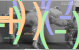
\includegraphics[width=.9\linewidth]{./figures/fig1_landmarks.png}
\caption{\label{fig:landmarks}\textbf{Video \chng{landmark tracking} and joint angle definitions.} White circles mark points of interest (``landmarks''). Movement was always rightwards. Labels show joint angles, defined as shown in the inset: straight joint (parallel segments) corresponds to zero; counter-clockwise \chng{joint} angles are positive. Forelimb \chng{joint} angle was used as a reference for temporal alignment, but did not enter the analysis.}
\end{figure}



The next step is to find the relevant temporal sequences of walking in the continuous videos.
Naturally, the trained network would only extract potentially useful landmark traces for episodes which resembled the training set, i.e. in episodes with a piglet moving perpendicular to the image axis, in lateral aspect and rightward direction.
We automatically extracted \(2597\) of such sequences by filtering for high \chng{landmark position} ``likelihood'' provided by DLC, low noise (i.e. steady landmark movement) and consistent, plausible inter-landmark distances.
We further applied an automatic algorithm to find footfalls and label stride cycles in the candidate episodes (\(4730\) cycles).
This procedure involved a start-end-matching optimization (using Procrustes superimposition, \textit{cf.} Ch. \ref{cpt:fourier_review}) to ensure that strides were indeed cyclical.
To further assess \chng{tracking data} quality, gait variables were automatically extracted.
Definition of these variables was chosen to simplify the automatic procedure, as follows.
Stride distance, frequency, and speed are trivial measures of the animal movement.
Duty factor is available for fore- and hindlimb, and measures the fraction of stride time in which the respective hoof is in ground contact.
Clearance is approximated by quantifying the ratio of flexion of each limb (one minus the quotient of minimum and maximum absolute hip-hoof-distance during the stride).
Head and torso angle are the stride-average angles of the snout-ear or withers-croup lines with respect to the coordinate system.
Hindlimb phase measures the time between hind- and forehoof touchdown, divided by the stride cycle duration.
Where applicable, spatiotemporal gait variables were prepared for analysis by converting them to dimensionless values \citep{Hof1996,Alexander1983} using the accumulated distance of landmarks along the snout-to-tailbase line of the animal as reference, extracted as stride average from the \chng{tracked} landmarks.
Only strides with plausible values (i.e. those which lie within the theoretical distribution of each parameter; \(1862\) cycles) where processed.
Manual inspection further boiled down the data set to 897 stride cycles (the others excluded for \chng{tracking} errors, multi-animal confusion, non-walking gait, intermittent or sidewards locomotion, or incompleteness).

Finally, \(368\) of the remaining strides from \(58\) animals were in the youngest age category (\(<10\ h\)) and thus selected for the present analysis, the data table is available online.


\subsection{Data Processing}
\label{sec:orgcb0a26c}

The landmark data provided by DLC was further processed for analysis.
Python code for the whole procedure is available (\nolinkurl{https://git.sr.ht/~falk/piglet_fcas}, Python version 3.11 at time of model calculation, \nolinkurl{https://www.python.org}).
First, joint angle profiles (i.e. joint angle values over time) were extracted for all relevant joints and for the total forelimb angle (croup-withers-hoof).
Shoulder, elbow, carpal, hip, stifle, and tarsal were the six joints sufficiently well \chng{tracked} and therefore considered relevant for analysis.
We then applied Fourier Series decomposition in the framework we previously termed Fourier Coefficient Affine Superimposition \citep[FCAS,][and Ch. \ref{cpt:fourier_review}]{Mielke2019}, a flexible procedure which subsumes the following steps.
Joint angle profiles are cyclic, i.e. periodical, and can therefore be transformed to the frequency domain with a Fourier Series decomposition (8 harmonics were deemed sufficient by visual comparison of raw and transformed/retransformed profiles).
In the frequency domain, the affine components (mean, amplitude, phase) of a joint angle profile are easily accessible \citep[\textit{cf.}][and Ch. \ref{cpt:fcas}]{Mielke2019}.
The forelimb angle served as reference to temporally align all cycles in the data set (removal of phase differences between different cycles; forelimb angle was not used further).
Then, mean and amplitude of the joint oscillations were isolated for all joint angles and are categorized as ``dynamic posture'' parameters.
Mean joint angle is the temporal average, whereas amplitude is related to effective range of motion (eROM).
The residual, i.e. differences captured by non-affine Fourier coefficients, can be categorized as ``coordination'' \emph{sensu stricto} (it measures the precise temporal succession of joint configurations).
In our case, there were
\(96\)
variables of coordination (6 \chng{joint} angles, 8 harmonics, real and imaginary) which were submitted to a PCA.
Only the first
\(12\)
coordination components (\(CC\)) were used for statistical analysis, capturing
\(80.2 \%\)
of the variability in coordination.

To summarize, FSD and FCAS served three purposes: (i) temporal alignment of the cyclic traces, (ii) separation of meaningful parameter categories (dynamic posture and coordination), and (iii) preparation for multivariate analysis via PCA.
Basic script code (Python, Matlab and R) to perform FCAS can be found on a dedicated git repository (\url{https://git.sr.ht/\~falk/fcas\_code}).


\bigskip
Information retention is generally a strength of this method.
FCAS and PCA are mathematical transformations, which means that the information content after transformation is theoretically identical to that prior to transformation (theoretically, because only a finite number of harmonics can be used, yet this is of little concern for continuous, smooth joint angle profiles).
The neglected PCs and the residual not captured by 8 harmonics were the only information from kinematics of the given joints to be lost in this procedure, and by definition these contain the least information.
Apart from that, all information present in the raw joint angle profiles enters the analysis.
Though we used a 2D dataset herein, the procedure could be applied equally well to \chng{joint} angles measured from 3D coordinate data \citep{Scott2022}.


Furthermore, all transformations are reversible, hence any analysis outcome can be translated back to kinematics with high accuracy.
Reversibility bares a lot of herein unused potential, for example for interpolating unobserved subject states or for inferring kinematics of fossil species by phylogenetic and morphometric bracketing.
Reversibility can also be of use when presenting raw joint angle profiles and their averages, as follows.
One crucial aspect of the FCAS procedure is temporal alignment of the joint angle profiles in the frequency domain.
In conventional temporal alignment, a single characteristic point in the stride cycle is chosen as a reference, wherein this is only ``characteristic'' for a certain part of one limb (e.g. left hindlimb hoof touchdown).
Temporal alignment to the hindhoof touchdown might cause distinct peaks in the forelimb angle joint profiles to occur at different relative points in the stride cycle (e.g. tarsal joint profiles in Fig. \ref{fig:raw_data}, lower half, green traces).
If profiles show such variable peak positions, then their average will have a wider, less pronounced (i.e. lower amplitude), and potentially unnatural peak.
For illustration, this is analogous to averaging two sine-waves of identical amplitude, but phase shifted: in the worst case, they cancel each other out (as in ``destructive interference'').
The problem is not restricted to pronounced peaks, but generally occurs if the temporal intra-limb coordination varies within a data set.
Using FCAS, it is possible to get a more representative average of the raw traces which has its amplitude conserved, but phase and mean \chng{joint} angle averaged.
This is enabled by transformation to the frequency domain, separation of affine components, removal of phase differences by shifting to average phase, profile averaging, followed by inverse transformation back to the time domain.
Because a set of profiles and phases may be calculated for each \chng{joint} angle individually, and because phase relations can differ between joints, there are the options to align based on one reference angle (e.g. the whole forelimb, as done herein) or minimize all phase differences across all joints.
Choosing the first option herein has implications: when plotting hindlimb joints aligned by a forelimb reference (as in Fig. \ref{fig:raw_data}, lower half), phases still differ, and the ``destructive interference'' problem might hamper averaging.
In such cases it is possible to apply an extra, joint-wise FCAS alignment for the sole purpose of generating meaningful averages.



\subsection{Statistical Modeling}
\label{sec:org7326405}
To summarize, four categories of variables were used for analysis:
\begin{itemize}
\item subject characteristics: age, sex, mass, birth weight category, size
\item spatiotemporal gait variables: distance, frequency, speed, clearance (fore-/hindlimb), duty factor (fore-/hindlimb), head angle, hindlimb phase
\item dynamic posture: mean joint angles and eROM for six joints
\item coordination: the residual after extraction of dynamic posture
\end{itemize}

Our guiding question for model design is whether a probabilistic, linear model is able to infer subject characteristics (specifically: age, mass, and size) from raw kinematics (expressed as dynamic posture and coordination) and spatiotemporal gait variables (collective variables).
Given the common conception that kinematics are a complex output of an individual motor system, this might be considered an ``inverse'' modeling approach (it is certainly an inversion of the model presented in Ch. \ref{cpt:statistics}).
The present analysis focused on three outcome variables (Fig. \ref{fig:observations}): mass (\(kg\)), size (\emph{arb. units}, from a PCA of marker distances), and age (\(h\)).
Though these outcome variables were specific per individual and recording session, we analyzed them ``per stride'' (i.e. there were multiple strides with identical subject measures on the outcome side).


The model formula is:
\begin{equation} \theta \sim v_{1}\cdot\alpha + v_{s}\cdot\beta_{s} + \sum\limits_{G} v_{g}\cdot\beta_{g} + \sum\limits_{P}  v_{p}\cdot\beta_{p} +  \sum\limits_{C} v_{c}\cdot\beta_{c} + v_{1}\cdot\epsilon \label{eq:model} \end{equation}
Herein, \(\theta\) is either of the outcome subject characteristics, \(\beta\) are slopes associated with the model parameters (\(s\) sex, \(G\) spatiotemporal gait variables, \(P\) dynamic posture, \(C\) coordination), \(v\) are data vectors (e.g. \(v_{1}\) is a vector of ones for the intercept \(\alpha\) and model residual \(\epsilon\), and \(v_{s}\) is a boolean vector coding for subjects of `sex == male`).
The models have a total number of 36 degrees of freedom.
Priors (i.e. \emph{a priori} assigned distributions) for all slopes were Normal distributions with mean and standard deviation corresponding to the mean and two times standard deviation of all observed values of each parameter; logarithmic transform was applied where necessary.
The observable (``likelihood'') prior for \(\theta\) was a Student's T distribution (allows for wider-than-normal tails and robust regression) with a Gamma distributed \(\nu\) (degrees of freedom); \(\epsilon\) was modeled to be a Half Cauchy distribution.
The model was implemented using the Python library ``PyMC'' \citep[different versions up to 5.10.2;][]{Salvatier2016}.


To re-emphasize, dynamic posture and coordination together effectively capture all the kinematic information of the stride.
Hence, we train the predictor model with all kinematics, spatiotemporal gait variables, and sex.
Birth weight category (LBW, NBW) is a filter parameter: we split our data set into LBW strides and two NBW subsets (training and validation).
Training is performed by MCMC sampling (`sample` function in PyMC), and a No U-Turn sampler was set to sample with \(32\) chains, each \(2^{14}\) tuning and equally many sampling steps.
All post-hoc model checks confirmed convergence (inspection of traces, \(bfmi>0.94\) for all chains, Gelman-Rubin statistics \(\approx 1\) for all parameters, sufficient effective sample size).
Model comparison was performed (cf. Ch. \ref{cpt:statistics}), iteratively leaving out model parameters or replacing some by meaningful combinations (e.g. duty factor combined for fore- and hindlimb).
However, because we follow an ``all in'' strategy, the results have little instructive value for model construction: we might thus have retained parameters which are numerically unimportant for the NBW-only models.



\begin{figure}[p]
\centering
\includegraphics[width=.9\linewidth]{./figures/histograms_observed.pdf}
\caption{\label{fig:observations}\textbf{Histogram of observations.} Trivially, the LBW group measured the lowest body masses in the data set. This correlated with a lower body size, whereas age is rather uniformly sampled for all study groups. Recordings happened opportunistically within the first ten life hours of the animals, repeated measurements were possible. Number of strides per class are indicated in brackets on the legend. Bar heights are scaled by sample size to show relative value distributions.}
\end{figure}


The data set of \(N = 368\) strides was split into three categories:
(i) the NBW training set as reference with \(N = 294\) strides,
(ii) the NBW validation set (\(N = 35\) strides), which is a random subset of NBW strides, approximately equal in size to
(iii) the LBW test set with \(N = 39\) strides.

The model was thus trained with a set of \(294\) NBW training strides (i).
Inferences (model ``predictions'') were then done per stride, for all observed strides (NBW training, NBW validation, and LBW test), iteratively using the `pymc.sample\_posterior\_predictive` function in PyMC after setting all the data arrays to the actual observed values for one given stride (using `pymc.set\_data`).
The number of predictions usually matches the number of training samples, which means that all posterior information is used to construct the prediction distributions.
We would thus retrieve mass, size, and age predictions (i.e. probabilistic inference) for each stride in the data set, which were then compared to the known, actual mass, size, and age.


All procedures, code, data, and this manuscript are available online \newline (\url{https://git.sr.ht/\~falk/piglet\_fcas}).

\FloatBarrier
\clearpage
\section{Results}
\label{results_22}
The present analysis is centered around a linear model which is designed to infer mass, size, and age (subject characteristics) from an extensive set of kinematic parameters from 2D videos.
The numbers provided by the model sampling are equally extensive, and will only be reported in brief.
The key purpose of the model is posterior predictive sampling of the LBW strides which were left out of the model, and which are analyzed in detail below.


\bigskip

\begin{figure}[p]
\centering
\includegraphics[width=.9\linewidth]{./figures/raw_profile_comparison.pdf}
\caption{\label{fig:raw_data}\textbf{Joint angle profiles per joint, grouped by birth weight category.} A \chng{joint} angle of zero would be a fully extended (i.e. straight) joint. Thick lines represent the average profiles, dashed lines indicate the average of the opposite birth weight group for comparison. Colored, shaded lines show all raw profiles available for the present analysis. Temporal alignment was done based on total forelimb angle (see methods), yet for the shown hindlimb averages (but not for the raw profiles), a separate alignment of the hindlimb was performed.}
\end{figure}

To assess whether there are qualitative differences between the birth weight categories, one can compare the joint angle profiles (i.e. raw, angular kinematics) on which the present analysis was performed (Fig. \ref{fig:raw_data}).
The intra-group variability clearly exceeds the differences between groups, although it must be emphasized that groups are heterogeneous (with regard to age, speed, etc.), which might lead to a bias if composition of LBW and NBW data differs.
LBW walk with a more flexed hindlimb posture, as indicated by the parallelly offset average hip, stifle, and tarsal profiles.
Additionally, NBW individuals on average seem to set the shoulder at a more extended \chng{joint} angle.
No differences in coordination are apparent (which would manifest in altered temporal structure of the profiles).
These findings indicate that LBW kinematics are hardly distinguishable from NBW kinematics by qualitative, visual assessment, which is at least in part be due to high variability.



\bigskip

\begin{table}[p]
\caption{\label{tab:modelresults}\textbf{Detailed modeling results.} Asterisk (*) indicates slopes for which the credible interval did not include zero. FL: forelimb, HL: hindlimb, dyn.p.: dynamic posture, coord.: coordination, diml.: dimensionless, d.s.: dimensionless stride, eROM: effective range of motion.}
\linespread{1} % Line spacing - Palatino needs more space between lines
\centering
\begin{footnotesize}
\begin{tabular}{rllllll}
 & category & parameter & age (h) & age (log) & size PC1 & mass (kg)\\\empty
\hline
0 & model & intercept & \(+4.86\) & \(+1.68\) & \(-3.25\) & \(+1.38\)\\\empty
1 & subject & female \(\rightarrow\) male & \(+0.05\) & \(+0.00\) & \(-0.38\) * & \(-0.04\)\\\empty
2 & gait & log. FL clearance & \(-0.10\) & \(-0.08\) & \(+0.09\) & \(-0.02\)\\\empty
3 & gait & log. HL clearance & \(+0.94\) * & \(+0.32\) * & \(-0.65\) * & \(-0.15\) *\\\empty
4 & gait & FL duty factor & \(+1.11\) & \(+0.37\) & \(+0.18\) & \(+0.07\)\\\empty
5 & gait & HL duty factor & \(+0.67\) & \(+0.24\) & \(+0.85\) * & \(+0.11\)\\\empty
6 & gait & d.s. distance & \(+1.32\) & \(+0.31\) & \(+0.45\) & \(+0.18\)\\\empty
7 & gait & d.s. frequency & \(+3.12\) & \(+1.43\) & \(+1.62\) & \(+0.15\)\\\empty
8 & gait & diml. speed & \(-1.10\) & \(-0.64\) & \(+0.82\) & \(+0.00\)\\\empty
9 & gait & hindlimb phase & \(-2.04\) & \(-0.56\) & \(-1.98\) & \(+0.05\)\\\empty
10 & gait & head angle & \(+0.26\) & \(+0.14\) & \(+1.44\) * & \(+0.18\)\\\empty
11 & dyn.p. & mean hip angle & \(+2.55\) * & \(+0.59\) * & \(-1.07\) * & \(-0.45\) *\\\empty
12 & dyn.p. & hip eROM & \(+2.64\) & \(+0.94\) & \(-1.34\) & \(-0.52\) *\\\empty
13 & dyn.p. & mean stifle angle & \(+0.67\) & \(+0.10\) & \(-2.01\) * & \(-0.12\)\\\empty
14 & dyn.p. & stifle eROM & \(-1.85\) & \(-0.22\) & \(-1.66\) * & \(-0.13\)\\\empty
15 & dyn.p. & mean tarsal angle & \(-1.18\) & \(-0.59\) & \(+0.44\) & \(+0.23\) *\\\empty
16 & dyn.p. & tarsal eROM & \(-1.92\) & \(-0.88\) * & \(+2.98\) * & \(+0.60\) *\\\empty
17 & dyn.p. & mean shoulder angle & \(+1.06\) & \(+0.07\) & \(+0.47\) & \(+0.06\)\\\empty
18 & dyn.p. & shoulder eROM & \(-0.34\) & \(-0.17\) & \(-0.65\) & \(+0.01\)\\\empty
19 & dyn.p. & mean elbow angle & \(-1.00\) & \(-0.55\) & \(+2.79\) * & \(+0.20\)\\\empty
20 & dyn.p. & elbow eROM & \(+3.22\) & \(+0.96\) & \(+0.11\) & \(-0.30\)\\\empty
21 & dyn.p. & mean carpal angle & \(-2.08\) * & \(-0.98\) * & \(+1.69\) * & \(+0.04\)\\\empty
22 & dyn.p. & carpal eROM & \(-0.24\) & \(+0.21\) & \(-0.84\) & \(+0.16\)\\\empty
23 & coord. & CC1 & \(+0.60\) & \(+0.31\) * & \(+0.10\) & \(-0.05\)\\\empty
24 & coord. & CC2 & \(+0.50\) & \(+0.15\) & \(-0.24\) & \(-0.08\)\\\empty
25 & coord. & CC3 & \(-0.25\) & \(+0.00\) & \(+0.88\) * & \(+0.07\)\\\empty
26 & coord. & CC4 & \(-0.62\) & \(-0.26\) & \(+0.13\) & \(+0.04\)\\\empty
27 & coord. & CC5 & \(-0.84\) & \(-0.25\) & \(-0.16\) & \(+0.04\)\\\empty
28 & coord. & CC6 & \(-1.49\) & \(-0.51\) * & \(-0.10\) & \(+0.07\)\\\empty
29 & coord. & CC7 & \(+0.24\) & \(+0.22\) & \(-0.76\) & \(-0.08\)\\\empty
30 & coord. & CC8 & \(-1.19\) & \(-0.24\) & \(-0.51\) & \(+0.02\)\\\empty
31 & coord. & CC9 & \(-2.96\) * & \(-0.83\) * & \(+0.66\) & \(+0.06\)\\\empty
32 & coord. & CC10 & \(-0.22\) & \(+0.06\) & \(-0.60\) & \(+0.02\)\\\empty
33 & coord. & CC11 & \(-2.05\) * & \(-0.67\) * & \(+0.10\) & \(+0.08\)\\\empty
34 & coord. & CC12 & \(-0.03\) & \(-0.10\) & \(+0.35\) & \(-0.01\)\\\empty
35 & model & \(\epsilon\) & \(\pm 1.81\) & \(\pm 0.56\) & \(\pm 0.98\) & \(\pm 0.20\)\\\empty
\end{tabular}
\end{footnotesize}
\linespread{2} % Line spacing - Palatino needs more space between lines
\end{table}



A quantitative comparison of variable kinematic measurements can be achieved with probabilistic linear models.
For the purpose of predictive sampling, we train models to describe the interrelations of kinematic parameters and subject characteristics in NBW piglets.
The outcome of MCMC sampling of a linear model are value distributions for slopes, which in our case indicated how certain kinematic parameters are associated with a change in mass, size, and age (Tab. \ref{tab:modelresults}; Fig. \ref{fig:output_effects}).
Of the gait- or coordination parameters, only hindlimb clearance was correlated with differences in animal mass.
Mass was also associated with changes in the dynamic posture of the hip and tarsal.
For size, the model inferred associations with head angle, hindlimb duty factor and clearance, and one coordination component (CC3), as well as changes in the fore- and hindlimb posture and an effect of sex.
Finally, age was associated with an increase in forelimb clearance, potential changes at the stifle and carpal, and several coordination components (CC9, CC11).
Some eROM slope distributions for age were high in average magnitude, but variable (the ``credible interval'' contained zero).
\chng{More details on the model input and output are discussed in a supplementary analysis to this chapter (Ch. \ref{supp:linearmodels}).}
These model results provide detailed insight into parameter interrelations in the present data set and indicate which of the parameters are the relevant ones to infer a given subject attribute in predictive sampling.



%\bigskip
\FloatBarrier
Performing in-sample and out-of-sample predictive inference with the models trained on NBW strides elucidated if and how left-out strides differed from NBW model expectation (Fig. \ref{fig:predictions}).
Note that, to capture variance (i.e. uncertainty in the prediction), each stride was sampled repeatedly.

\begin{figure}[p]
\centering
\includegraphics[width=.9\linewidth]{./figures/histograms_prediction_comparison.pdf}
\caption{\label{fig:predictions}\textbf{Predictive sampling of subject characteristics.} For all included subject characteristics, models which were trained on NBW strides correctly inferred the training data (gray) and values from the validation set (blue). In contrast, the same models wrongly inferred the characteristics of LBW subjects (orange). The \(x\)-axes show the difference (\(\Delta\)) between actual and predicted values per prediction. To facilitate comparison, histogram heights are again normalized per category.}
\end{figure}


Out-of-sample inferences for the \emph{NBW validation set} matched those of in-sample NBW inference in terms of average values and standard deviation for all modeled outcome variables, which confirms that inference of subject characteristics from kinematics is possible.
In contrast, inferences for the \emph{test set} of LBW strides did not match those of the NBW training set.
Low birth weight animals were inferred to be on average \(0.44 kg\) heavier than actual, and their size was overestimated (\(+1.71\)
units).
Both faults matched the actual differences in magnitude (\emph{cf.} methods, Fig. \ref{fig:observations}).
In contrast, the age inference for the low birth weight subjects were not normally distributed: most ages were correctly inferred from stride-wise kinematics, but ages for some strides were underestimated.
The underestimation of those strides quantified to just below five hours.

In summary, the NBW-trained model ``guesses'' the size and mass of the animals producing LBW strides to be ``normal'' (although they are not), which indicates that these defining features of LBW do not reflect in altered kinematics.
However, age inference is non-normal, i.e. some strides are classified as typical for animals of younger than actual age.
\bigskip

\begin{change}
To assess whether out-of-sample prediction is a valid and unbiased method to infer group differences, we extracted additional indicator quantities from the linear models.
An in-depth analysis can be found at the end of this chapter (Ch. \ref{supp:linearmodels}).
Theoretical considerations identify several criteria which, if not met, can obscure an actual group difference (which consequently does not emerge in the prediction output).
These criteria are differences in the input parameter distribution, slope magnitude, and low residual variability; in addition, model complexity and a limited sample size can be prohibitive.
For the age model, our considerations confirm that a predicted difference is robust, and we were able to evaluate which of the model parameters might cause the underestimation of some strides (primarily hindlimb clearance and hip angle).
In the models of size and body mass, some of the criteria are not met.
Model complexity and sample size might restrict clarity of both models' outcomes to an uncertain degree.
In the body mass model, the residual variability is high, which blurs potential differences in the predictions (Ch. \ref{supp:linearmodels}, Fig. \ref{fig:output_effects}).
In the size model, there are some positive and some negative effects which seem to cancel out (which might be evidence for size-dependent alternative locomotor strategies; Figs. \ref{fig:input_distributions}, \ref{fig:output_effects}).
We observed few significant effects related to the coordination parameters, indicating that coordination patterns are for the most part indifferent to age, size, and mass.


This lends some support to the outcome of the age model, and points towards the limiting factors in case of the other two models.

\end{change}
\bigskip


\begin{table}[p]
\caption{\label{tab:prediction}\textbf{Age inference per LBW animal} (compared to NBW average, last row). \(\Delta\): ``inferred - actual'' difference. Underestimation is defined as \(\Delta < 0\), ``count'': per stride, ``rate'': per predictive sample. \(h\): hours, \(std\): standard deviation.}
\centering
\begin{tabular}{|l|c|c|c|c|c|c|}
\hline
  \textbf{piglet} & \textbf{age} & \textbf{strides} & \multicolumn{2}{c|}{\textbf{underestimation}} & \textbf{pred. mean} \(\Delta\) & \textbf{pred. std}
  \\\hline \empty & h &  & count & ratio & h & h\\\empty
\hline \hline
b23 & 2.0 & 6 & 0 & 0.29 & 1.13 & 2.00\\\empty
b15 & 2.9 & 5 & 0 & 0.37 & 0.68 & 1.96\\\empty
b76 & 3.1 & 4 & 0 & 0.39 & 0.57 & 2.01\\\empty
b74 & 4.2 & 7 & 1 & 0.40 & 0.52 & 1.97\\\empty
1794.5 & 5.6 & 5 & 5 & 0.90 & -2.57 & 1.99\\\empty
b58 & 7.8 & 3 & 3 & 0.91 & -2.85 & 2.00\\\empty
b19v2 & 9.8 & 1 & 1 & 1.00 & -6.14 & 1.99\\\empty
b56 & 9.9 & 8 & 8 & 0.99 & -4.58 & 1.96\\\empty
\hline
<all NBW> & <3.8> & 329 & 158 & 0.49 & -0.03 & 1.95\\\empty
\hline
\end{tabular}
\end{table}


To find out whether the offset age inference was related to certain individuals, or certain strides from different individuals, we grouped the inferences per stride or subject and calculated the chance of over- or underestimating age.
Of the
\(8\)
low birth weight subjects who contributed
\(39\)
strides,
\(4\)
individuals were consistently underestimated (Tab. \ref{tab:prediction}).
Consistently means that more than \(75 \%\) of all predictive samples were below actual age, and that the ages for a majority of strides were on average underestimated.
The magnitude of underestimation was between two and five hours.
Curiously, those were the individuals recorded at a slightly higher age (\(> 5\) hours).
Overestimation in the other four LBW individuals was also consistent, but less so (less extreme underestimation rate, mean \(\Delta < 2\ h\)).
Standard deviation of the estimates did not vary across individuals or birth weight categories.

We conclude that underestimation of age is consistent over multiple strides of the same individual, and thus individual-specific.

\FloatBarrier
\clearpage
\section{Discussion}
\label{discussion_22}

Birth weight variability in piglets is considerable.
The average birth weight of a new born piglet in our data set is just above a kilo, yet the span within a litter is typically above \(800\ g\).
Size ranges are accordingly high.
Low birth weight is often associated with low vitality \citep{Baxter2008,Hales2013,Muns2013}, and this supposedly correlates with deficient locomotion.
Previous studies reported behavioral, physiological, and other differences for piglets of low body mass which could affect locomotion \citep{Quiniou2002,Muns2013,VandenHole2018b,Alvarenga2013,VandenHole2018,Roelofs2019}.
One might therefore anticipate differences in how these newborn animals move their more or less heavy bodies, which is the immediate outcome of motor control.
Top-down, direct, visual assessment could justify the hypothesis that LBW walking kinematics are somehow different from ``normal'' \citep{DEath2012}.
Yet that is (i) hard to assess due to high behavioral variability and (ii) trivially expected given the adaptation to different physical properties of their body: gravitational force is a predominant constraint of locomotion, and it simply scales with animal weight \citep{Aerts2023}.
The overarching question is whether low or critically low birth weight can be quantitatively associated with a deficit in locomotion.


However, we observe little qualitative difference in LBW and NBW kinematics (Fig. \ref{fig:raw_data}).
There is a small difference when averaging hindlimb posture, which might be trivially explained by heterogeneous group composition (but see below).
This is further supported by the fact that our models were unable to correctly retro-infer either mass or size from blindly provided kinematic parameters, including coordination.
Strides from LBW animals were estimated to come from an animal with a ``normal'' mass and size (Fig. \ref{fig:predictions}).
This suggests that low body mass or small size can not be causal for altered 2D kinematics, and it raises doubts whether there are any deficits in coordination and control.
Within the range of kinematic variability, we observe LBW animals perfectly \emph{capable} of normal posture, coordination, and overall stride results (collective variables).
Note that this does not rule out problems of balance, stability, or endurance.


We do see differences for LBW compared to NBW recordings, nonetheless.
First, a difference in sample size.
There are much fewer valid LBW strides in our data set: only \(39\) of \(368\) observations are LBW.
This could be interpreted as evidence for a lower capacity  of LBW to produce normal locomotion (i.e. they succeed in this locomotor task less frequently, despite equal potential).
Yet there are proximal, trivial explanations: based on conventions, the \(10 \%\) lower quantile of birth weights in a litter is considered LBW, and there is a hard cap of \(800\ g\).
The resulting share is equal in our training set for video \chng{tracking}, and in the final data set, because of pseudo-random, opportunistic sampling on-site (i.e. recording work was permanent, yet determined by farrowing and feeding of the subjects).
The minority of LBW training videos might lead to an under-learning of those animals, reduced \chng{landmark tracking} quality and therefore an exclusion bias for ``non-normal'' individuals.
Though it seems unlikely, we cannot rule out reduced locomotor endurance in LBWs, because the present data set is unsuited to count the occurrence of locomotor behavior.
On the other hand, the strict stride filtering criteria for ``good'' kinematics may have involuntarily filtered out deficient individuals.
Our conclusion that low birth weight individuals are non-deficient is strictly tied to the definition of the low birth weight category, which is herein based on weight criteria and did not regard phenotypic indicators of intra-uterine growth restriction \citep[which we did not record, \textit{cf.}][]{Amdi2013}.


A second difference of LBW locomotion is that the age is underestimated for strides of some, but not all individuals.
Prediction is consistent per individual, although no subject characteristics except sex entered the model (``blind'' inference).
This supports the hypothesis that locomotor development is sometimes delayed in LBWs.
Delayed development does not necessarily corroborate the hypothesis of locomotor deficiency in LBW: we would expect truly deficient strides to be substantially different from the data trained to the model, making it ``unpredictable'' (i.e. higher variance of posterior samples).
Instead, the predictions are consistent for repeated measures of an individual, without notable increase in variance.
For the affected subjects, we can even quantify a delay of less than five hours, which could nevertheless be critical given the rapid maturation of locomotor behavior in this species \citep{VandenHole2017} and the importance of postnatal competition \citep{Litten2003}.


Note however that the causality might be inverse.
We measured age underestimation only in the case of the individuals which were recorded late within our sampling time frame (age \(> 5\ h\), Tab. \ref{tab:prediction}).
This is consistent with prior evidence that energy reserves are depleted after birth (normal locomotion) but not replenished after four hours in the case of LBW \citep{LeDividich2017,VandenHole2019}.
Assuming that this is the case, i.e. energy reserves are depleted, we would expect two effects: (i) the animal might succeed in the locomotor task less frequently (not quantified, see above), and (ii) the kinematics might be altered, which we observed.
The present model was trained from NBW data and thereby tuned to kinematic development from animals with normal energy levels (therefore it can correctly infer age from kinematics in NBW).
That same model quantifies the potentially energy-deficient animals as younger.
It might be that energy deficiency co-incidentally causes effects which are exactly opposite to the changes that piglet kinematics undergo in normal development.
However, the more likely explanation is an actual delay or a temporary halt in development.
Failure of the LBW to compete in the first hours are sufficient to explain reduced intake \citep{Amdi2013}, the absolute size and mass difference alone might be crucial, and an immediate question which we cannot address with the present data set is whether and how (fast, likely) animals would recover from the delay.
Alternatively, there might be a technical artifact in probabilistic sampling \citep[``shrinkage'', \textit{cf.}][]{Gelman2013} which caused the underestimation of ``above average age'' individuals.
Yet this is an unlikely explanation, given that shrinkage would apply equally to NBWs, and inversely to the opposite, younger subjects.
Finally, with only eight LBW individuals, we cannot exclude co-incidence in which individuals are affected.

Neither of these technical explanations puts doubt on the clarity of the initial finding: a subset of the low birth weight individuals produced locomotor behavior which is quantitatively similar to that of younger individuals.


A corollary question is which patterns in the kinematic variables cause the different age inferences.
We report high magnitude (but also highly variable, i.e. ``non-significant'') slopes inferred from the age model (Tab. \ref{tab:modelresults} \chng{and Fig. \ref{fig:output_effects}}).
Note that these slopes solely reflect effects within the NBW data subset.
We also observed slight differences in the average hindlimb dynamic posture (Fig. \ref{fig:raw_data}).
In fact, a more flexed hindlimb is typical for the youngest animals of both birth weight categories.
\chng{This is further supported by the observation that hindlimb clearance and mean hip angle have a pronounced effect in the age model (Fig. \ref{fig:output_effects}).}
We emphasized potential differences in group composition to explain that (e.g. sex effect in the ``size'' model), and different age per group might be a proximal explanation for the non-normal age inference in LBW.
However, the average age of LBW animals (\(5.3 h\)) in our data set is nominally above that of NBW (\(3.8 h\)), which is a discrepancy with the age underestimation.
Yet if we assume that the hypothesis of delayed locomotor development is correct, the nominal age would be misleading, and LBW effectively behave similar to younger animals.
This can explain the apparent discrepancy in age group composition and age predictions from kinematics.
Though many other parameters also entered the probabilistic model and influenced the model outcome, \chng{our data suggests that dynamic posture, especially of the hindlimb, might be the major proxy for perinatal maturation (Fig. \ref{fig:output_effects})}


\bigskip

The findings discussed above are enabled by ``inverse'' modeling of subject characteristics as a function of kinematic parameters, using probabilistic models.
The models do reveal various parameter associations, yet the top down (repeated) testing with the chosen model structure complicates drawing definite conclusions \citep[e.g. we observed a sex effect on size, but opposite of what other studies have reported,][we conclude males in our study were just smaller by chance]{Baxter2012}.
Instead, the demonstrated predictive modeling strategy \citep{Shmueli2010} leverages the potential of probabilistic models to perform out-of-sample prediction (via separation of the LBW test group).
\chng{This strategy is limited by a major asymmetry: in case the prediction shows differences, they are most likely robust, yet ``non-effects'' could be caused by unfavorable dataset characteristics (Ch. \ref{supp:linearmodels}).}
Non-probabilistic modeling could equally serve to predict values, but it cannot generate parameter distributions (as in the bimodal age predictions, Fig. \ref{fig:predictions}).
Our probabilistic models implicitly regard ``non-significant'' parameter slopes \chng{(Fig. \ref{fig:output_effects})}, which are usually neglected in standard hypothesis testing (such as the high magnitude, highly variable joint ROM quantities, which might nevertheless have relevance for age prediction in case they are correlated and add up).
The data transformations and predictive modeling strategy we applied herein hold further potential for inferring kinematics, for example by morphometric bracketing of extinct taxa.
For that purpose, one would train a model to infer dynamic posture and coordination from a given range of morphometrics, predict samples for specific morphometrics in that range, and convert the samples back to (3D) joint angle profiles which could be animated.


There is a conceptual hierarchy, but no clear causality, with regard to modeling parameter dependencies in quantitative studies of locomotion.
For example, animals might increase the hip angle (posture) and the temporal pattern in the joint angle profiles (coordination) to reach higher speeds (spatiotemporal gait variables), but the speed they reach might depend on age (i.e. maturation, a subject parameter).
But maturation and age might also influence the speed without changing dynamic posture or coordination, simply because the animal grows and increases strength.
Age might also affect dynamic posture and coordination directly, for example if dimensionless speed stays constant but clearance changes with age.
Reducing clearance can increase speed (less unnecessary hoof lifting) or reduce it (higher duty factor), which can be distinguished by the other parameters.
This complex interrelation of spatiotemporal quantities complicates the intuitive modeling strategy, which involves using subject characteristics as a factor to predict a multivariate block of spatiotemporal gait variables and kinematics.
In our experience, model residuals in such models are high, multiple testing can yield putatively co-incidental significances, cross-dependencies within the multivariate data set might be underestimated, and sample size requirements are high.
And even under ideal circumstances: chances are that such models would yield \emph{some} age effect, even with random data.

\medskip
In contrast, the strategy applied herein is related to the question: ``given the complete kinematic output of a behavior, can we infer subject characteristics of the animal producing it?''
We used probabilistic, predictive models, which are able to capture intrinsic variability of the process, and addressed specific categorical questions (NBW/LBW differences) by out-of-sample predictions.
We demonstrated that, in the first ten hours of piglet life, (1) kinematics seem to be indifferent to low body mass and size, and (2) locomotion of some LBW individuals could be explained by a delay in locomotor maturation which is initiated \emph{post partum}.


\clearpage
\section{Supplementary Analysis}\label{supp:linearmodels}
\begin{change}
The key findings in this chapter are based on an analysis which uses the statistical model of one subset of the data for predictive inference on another subset, a strategy which demands justification.
\begin{itemize}
\item Is the model actually \textit{capable} of finding differences?
\item Under which circumstances will group differences arise?
\item Is there a bias in the modeling procedure, for example to not find all differences?
\end{itemize}
Answering these questions requires a rather technical, in-depth analysis of the model outcome.

One important constraint is that the models herein are linear, i.e. of the form
\[y = a + b_1 \cdot x_1 + b_2 \cdot x_2 + \ldots + b_m \cdot x_m + \epsilon = a + \sum\limits_k b_k \cdot x_k + \epsilon\]

Herein, \(y\) is one of the outcome variables (observed; age, size, or mass), \(a\) is the intercept, \(b_i\) are the slopes, \(x_i\) are the different input parameters (observed; spatiotemporal gait variables, dynamic posture, and coordination measures), and finally \(\epsilon\) is the model residual (unexplained variation, including for example measurement inaccuracy).
As I have demonstrated \href{http://mielke-bio.info/falk/posts/33.linearmodels}{elsewhere} \citep{Mielke2024lm}, there are some \textbf{criteria} which are necessary (but not sufficient by themselves) for the model to predict a difference.
Given there is a...
\begin{enumerate}
\item significant difference between the study groups in the distributions of input variables
\item high enough slope magnitude (``steepness'')
\item limited model complexity/size, i.e. moderate number of (other) slopes
\item low residual variation
\item sufficient sample size
\end{enumerate}

... then we can find differences.
An example where all these conditions are met is the age model, above.
In case one of these conditions is not met, a difference between the study groups might be obscured (yet note that the criteria are on a continuum, some cases might not be clear-cut).
From theoretical considerations alone, this situation is biased.
Differences in out-of-sample prediction must have passed the criteria above, and are therefore robust.
Yet on the other hand, \textit{``the absence of evidence is not the evidence of absence''}: if for example the sample size is low, or the residual variation is high, the model's prediction might miss an actual effect.
This situation is somewhat analogous to classical hypothesis testing, where we quantify the chance of falsely rejecting a null hypothesis such as ``groups were samples from the same distribution''.

\begin{figure}[b]
  \caption{ \textbf{Observed model parameter input distributions} (\textit{next page}).
For each model parameter (rows), observations are indicated by tick marks for the two study groups (NBW: gray, LBW: orange). Values were standardized on population level (i.e. mean-centered and scaled by standard deviation). Significance between the distributions (indicated by asterisk) was determined by a two-sample rank sum test. }
\end{figure}

\addtocounter{figure}{-1}
\begin{figure}[p!]
\centering
\includegraphics[width=16cm]{./figures/input_distribution_differences.pdf}
\caption{\label{fig:input_distributions}\textbf{Observed model parameter input distributions.} \textit{See previous page.}}
\end{figure}



\begin{figure}[p!]
\centering
\includegraphics[width=16cm]{./figures/output_effectsize.pdf}
\caption{\label{fig:output_effects}\textbf{Effects of each input parameter on the model output.} \textit{See next page.} }
\end{figure}
\addtocounter{figure}{-1}
\begin{figure}[t]
  \caption{ \textbf{Effects of each input parameter on the model output} (\textit{previous page}).
Effect size is calculated as the data range (difference between \(2.5\%\) and \(97.5\%\) data quantiles) multiplied by the slope distributions (from model sampling). Effect magnitude and therefore relevance is visualized by red shading, effects which are different from zero (\(95\%\) HDI) are also marked by an asterisk. The residual (last row) is determined as the difference of the actual parameter observations and the model result. }
\end{figure}



The available modeling framework enables some extra insights on why the prediction of piglet subject characteristics appeared as it did.
Firstly, we can compare the input distributions (criterion 1, above) of the observational groups, to identify those model parameters which actually influence the predictions (Fig. \ref{fig:input_distributions}).
Secondly, we can calculate the absolute effect of each parameter on the predicted outcome (slope magnitude, criterion 2), by multiplying the parameter magnitude with the according slope (Fig. \ref{fig:output_effects}; this works because \(\Delta y \sim b_i \cdot \Delta x_i\)).
Thirdly, we can quantify the model residual (criterion 4; Fig. \ref{fig:output_effects}, last row).
The other criteria (model complexity and sample size) are predetermined in this modeling application, and have an unknown influence on the outcome.

For the \textbf{age model}, we observe a low residual variance, and there are two parameters which are significantly different between NBW / LBW \textit{and} have a high slope (those are hindlimb clearance and hip angle).
Notably, there is hardly any difference in the observed coordination parameters.
For the model of \textbf{body mass}, the same parameters seem to have relevant slopes, yet the model residual is much higher and likely prohibits conclusive differences in the probabilistic prediction.
Other slopes seem to have significant effect in the NBW group (hip and tarsal eROM), yet the input distributions (i.e. NBW and LBW observations) do not differ, and so their effect is irrelevant for prediction of mass.
For the \textbf{size model}, we find some slopes with a negative effect on the output (hindlimb clearance, head angle, hip angle).
However, others with a positive effect (knee angle, tarsal eROM) possibly cancel this out for the overall prediction.
Like the previous one, this model contains significant slopes with nonetheless no difference in the input distribution.
We also compared the relative widths of effect size distributions, and found that ``dimensionless (relative) speed'' is most variable among trials: all animals use a variety of speeds, and apparently this can not be systematically associated with age, size, or mass.
It must be re-iterated that ``significance'' in these analyses merely provides a hint to guide the eye: the combination of a minor (non-significant) difference in an input parameter with a notable, only ``almost-significant'' effect size might still affect the probabilistic prediction.
Finally, the input distributions (Fig. \ref{fig:input_distributions}) are insightful by themselves for NBW / LBW comparison.
Some LBW parameters are bimodally distributed, which might be related to the prediction outcome for the age model.
We observe most differences in spatiotemporals (predominantly hindlimb-related), as well as in measures of dynamic posture and range of motion.
However, there are few significant effects of coordination parameters, and the remaining ones are cancelled out by a lack of difference in the observed coordination of LBW and NBW.


To summarize, we show that a detailed inspection of on the one hand the observed model input parameters, and on the other hand the effect ``lever'' of each parameter slope, warrants some caution about non-different predictions (as in the models of size and mass).
In those models, we cannot rule out that a larger sample size or an adjusted, potentially more selective model design might elucidate quantitative NBW/LBW differences.
On the other hand, inspection of the predictive age model confirms that finding differences by out-of-sample prediction is possible, and we could even relate those findings to specific model parameters.

\end{change}






\FloatBarrier
\clearpage
\section{Acknowledgements}
\label{sec:org2d8bfbc}
The author would like to thank Miriam Ayuso for organizing and participating in the recording sessions, as well as Laura Buyssens, Georgios Petrellis, Gunther Vrolix, Charlotte Vanden Hole, Denise Vogel and all students who joined for help during recordings.
A comment by Ann Hallemans stimulated the extra analysis, from which this chapter benefits a lot; thank you!
Maja Mielke provided valuable comments on the manuscript text, in fact for all three major versions of it, and I am very glad she did.


\FloatBarrier
\clearpage
% \bibliographystyle{apalike}
% \bibliography{literature.bib}




\cleartorightpage
\part{Inverse Dynamics}\label{pt:3}
% \chapter{Introduction: Inverse Dynamics}\label{cpt:dynamics_intro}
% \clearpage


\section{Abstract}
\label{sec:org46d1be2}
Here, I am going to write a summary of this extraordinary manuscript.

\clearpage

\section{Introduction}
\label{sec:orgd1de252}
Until this point, this thesis has been busy with methodological development in terms of measuring kinematics.
With Fourier-based methods and probabilistic models in place, one can
  (i) quantify measured kinematics
  (ii) simulate locomotion by predictive sampling of trained models.
This is a full grasp at \textbf{how animal segments move}.
Segments could be axial or peripheral parts of the animal which move as a unit (rigid- or pseudo-rigid bodies).


Another aspect of locomotion is \textbf{why segments move}.
This opens up the rabbit hole of elementary physics:
\begin{quote}
A rigid body will change its linear or angular momentum if there are external forces or external torques applied to it.
\end{quote}
This is also called the Conservation of Momentum.
And the study of the conservation of momentum is also called ``Dynamics'', which is the broad topic of this chapter.
Again, this will contain methodological considerations, backed up with actual measurements of at least a part of a piglet.

In a nutshell:
\begin{itemize}
\item Wrenches and quaternions are a useful computational tools for calculating rigid body dynamic models.
\item Balance Equations are the mathematical manifestation of conservation of momentum.
\item Reference frame considerations can simplify calculations; however, only static frame calculations result in correct joint moments.
\item Fictitious Forces are unbalanced change of momentum. If one intends to calculate balances in an accelerating frame, include four fictitious forces: D’Alambert, Euler, Coriolis, and the Centrifugal force.
\item Computed Tomography might be a shortcut to retrieve material constants which are crucial for the calculation of dynamics.
\end{itemize}


Again, a lot of the herein summarized work is physics textbook knowledge, re-formulated to be more readily applied to animal locomotion.
Again, the premise is ``falsification'': instead of assuming that CT scan data is useful to easily extract inertial properties of body segments, I will attempt to find flaws in that procedure.


\subsection{Dynamics: Theory}
\label{sec:org6d0e666}
\begin{itemize}
\item forward and inverse dynamics
\end{itemize}

\subsection{Screw Theory and Wrenches}
\label{sec:orgfc04ba7}
Dumas 2004, Lynch and Park 2017

\subsection{Quaternions}
\label{sec:org65e1cb2}

\subsection{Balance of Forces and Moments}
\label{sec:org0ccd151}
conservation of linear and angular momentum (TODO check!)
\begin{itemize}
\item \(F_J = m\ddot{x} + \frac{\partial m}{\partial x} \dot{x}\dot{x} = m\ddot{x}\)
\item \(M_J = I\ddot{\omega} + \dot{\omega} \times I\dot{\omega}\)
\end{itemize}

\subsection{Mass}
\label{sec:org3ee3a48}
resistance to linear acceleration

\subsection{Mass Moment of Inertia}
\label{sec:org05fc151}
resistance to angular acceleration
Vector formula
Generalized Steiner
\subsubsection{Conventional Methods}
\label{sec:orgf0a43d8}
\subsubsection{Using CT scans}
\label{sec:org1a78e3f}
\citep{DuPlessis2013,Durston2022}

\subsection{Reference Frames and Ficticious Forces}
\label{sec:orge4c93d5}
Take home message: Make sure, in this and all that follows, in what reference frame parameters are defined and whether they were transformed.

D’Alambert Force, Euler force, Centrifugal force, Coriolis force

After all, this is how physicists formalize fictitious forces: I read that when Léon Foucault observed precession of his pendulum, no responsible external force could be found, but angular momentum of the pendulum changed. Coriolis Force rectified this discrepancy, and because Coriolis force comes with a rotating frame, this was evidence for the rotation of the earth.

Back to our question. Are there more than the four fictitious forces? Probably no. Remember the “five accelerations” derivation linked in the prequel notebook of this series. That derivation captures all the possible forms of momentum for which we have evidence.


I have encountered several types of definitions of fictitious forces during my initial attempts.

The first type is a practical one, which goes along the lines of “fictitious forces arise because an observer who is captured in the rotating frame is blind to the movement of the frame”. Yes, that is a valid description, but a disappointing definition: What else might the observer be blind to? How can we calculate something we are blind for? And why can’t I not always switch perspective in cases where I’m in charge of the data?

The second type of definition is a technical one: “fictitious forces need to be introduced to make balance equations work in the rotating reference frame”. That is also a valid point, yet it leaves similar questions as above: Which ones do I have to include when? Where do the formulas come from?

I have hinted at these aspects above. They certainly help to develop an intuition about fictitious forces, but for me they were not satisfactory. You can find these two categories scattered all over the Wikipedia articles about fictitious forces. Despite my rants herein, I’m not disappointed about Wikipedia, it is just sad that this confirmed my prior on that “Encyclopedia”. But I also see myself as a source of the problem: whereas for trained physicists it is often obvious which and how vectors add up, my humble, untrained mind needs some more explicit guidance. [update 2020/09/12] And although I’m using myself in a tautologous way here, those of you who read my first version of the notebook are witness that I could confidently ignore the D’Alambert force without noticing.

I found a third definition most convincing, yet it is more like a prescription than a definition. It is the one which I found in the workbooks by Frank Owen (five-term acceleration, see references).

Conceive a position vector to a point on a rigid body as a superimposition of the position vector of the reference frame attachment point (in static frame), and the movement of the point of interest relative to the attachment (in body frame).
Calculate component-wise time derivatives of that superimposed vector; use product rule, and make sure to incorporate time changes of reference frame basis vectors.
In the outcome, two acceleration components are intuitive cartesian superimpositions; the others depend on cross products of angular and linear motion parameters. Four of them are irritatingly labelled “fictitious”.
A corollary rule of thumb for those three: angular motion parameters (\(\omega\) and derivatives) stem from the static frame, whereas linear motion parameters (\(x\) and derivatives) are best seen in the body frame.

[update 2020/09/12] Finally, after having finished my work on this series of notebooks, I would like to attempt another definition, which I think captures the inverse dynamics standpoint: Instead of being forces, Fictitious Forces represent a change of the momentum which is not captured by kinematics in the observer’s frame of reference. Instead of writing them on the side of the external forces (of which I think as the cause of a momentum change), I tend to put them on the “effect” side and would rather call them “unbalanced change of momentum” (“unbalanced” as in “not part of the balance”).

I had to write a couple of notebooks to come to that conclusion, and would be glad if you like to follow through. The fourth one will explain this fourth definition in more detail.

This preparational notebook has solved some puzzles which I encountered when starting to learn about fictitious forces. Make sure to keep track of your reference frames and reference points. Good (i.e. explicit, structured, well commented) programming style can facilitate this. And remember that, even if you think it is obvious which parameters you took in which transformation, make sure that others can reproduce your line of thought.

With these tools at our hands, we can advance to elementary examples. I’ll start by isolating Euler, i.e. with an example that should show the Euler force in isolation, in the next notebook. If you don’t mind the explanations, feel free to skip ahead to the code from the application to a general (n-link) limb.


\subsection{Application: The N-Segment Piglet Limb}
\label{sec:org5321bfb}

\section{Results}
\label{sec:orgff6d7a6}
\subsection{Issue 1: Beam Hardening}
\label{sec:orgeb51aa9}
\subsection{Issue 2: Chemical Composition}
\label{sec:orgf412c36}
\begin{itemize}
\item water streaks on the scan
\end{itemize}
\subsection{Issue 3: Marker Artifacts}
\label{sec:orgdc3358c}
\begin{itemize}
\item helical scanning
\end{itemize}

\section{Discussion}
\label{sec:org4195f4b}
\subsection{Which Inertia Component is Relevant?}
\label{sec:orgb3e7c4f}


\section{Acknowledgements}
\label{sec:orgdc4f21e}
\pagebreak

% \bibliographystyle{apalike}
% \bibliography{literature.bib}


\chapter{Inverse Dynamics Workflow}\label{cpt:dynamics_workflow}
\clearpage


\section{Abstract}
\label{sec:org46d1be2}
Here, I am going to write a summary of this extraordinary manuscript.

\clearpage

\section{Introduction}
\label{sec:orgd1de252}
Until this point, this thesis has been busy with methodological development in terms of measuring kinematics.
With Fourier-based methods and probabilistic models in place, one can
  (i) quantify measured kinematics
  (ii) simulate locomotion by predictive sampling of trained models.
This is a full grasp at \textbf{how animal segments move}.
Segments could be axial or peripheral parts of the animal which move as a unit (rigid- or pseudo-rigid bodies).


Another aspect of locomotion is \textbf{why segments move}.
This opens up the rabbit hole of elementary physics:
\begin{quote}
A rigid body will change its linear or angular momentum if there are external forces or external torques applied to it.
\end{quote}
This is also called the Conservation of Momentum.
And the study of the conservation of momentum is also called ``Dynamics'', which is the broad topic of this chapter.
Again, this will contain methodological considerations, backed up with actual measurements of at least a part of a piglet.

In a nutshell:
\begin{itemize}
\item Wrenches and quaternions are a useful computational tools for calculating rigid body dynamic models.
\item Balance Equations are the mathematical manifestation of conservation of momentum.
\item Reference frame considerations can simplify calculations; however, only static frame calculations result in correct joint moments.
\item Fictitious Forces are unbalanced change of momentum. If one intends to calculate balances in an accelerating frame, include four fictitious forces: D’Alambert, Euler, Coriolis, and the Centrifugal force.
\item Computed Tomography might be a shortcut to retrieve material constants which are crucial for the calculation of dynamics.
\end{itemize}


Again, a lot of the herein summarized work is physics textbook knowledge, re-formulated to be more readily applied to animal locomotion.
Again, the premise is ``falsification'': instead of assuming that CT scan data is useful to easily extract inertial properties of body segments, I will attempt to find flaws in that procedure.


\subsection{Dynamics: Theory}
\label{sec:org6d0e666}
\begin{itemize}
\item forward and inverse dynamics
\end{itemize}

\subsection{Screw Theory and Wrenches}
\label{sec:orgfc04ba7}
Dumas 2004, Lynch and Park 2017

\subsection{Quaternions}
\label{sec:org65e1cb2}

\subsection{Balance of Forces and Moments}
\label{sec:org0ccd151}
conservation of linear and angular momentum (TODO check!)
\begin{itemize}
\item \(F_J = m\ddot{x} + \frac{\partial m}{\partial x} \dot{x}\dot{x} = m\ddot{x}\)
\item \(M_J = I\ddot{\omega} + \dot{\omega} \times I\dot{\omega}\)
\end{itemize}

\subsection{Mass}
\label{sec:org3ee3a48}
resistance to linear acceleration

\subsection{Mass Moment of Inertia}
\label{sec:org05fc151}
resistance to angular acceleration
Vector formula
Generalized Steiner
\subsubsection{Conventional Methods}
\label{sec:orgf0a43d8}
\subsubsection{Using CT scans}
\label{sec:org1a78e3f}
\citep{DuPlessis2013,Durston2022}

\subsection{Reference Frames and Ficticious Forces}
\label{sec:orge4c93d5}
Take home message: Make sure, in this and all that follows, in what reference frame parameters are defined and whether they were transformed.

D’Alambert Force, Euler force, Centrifugal force, Coriolis force

After all, this is how physicists formalize fictitious forces: I read that when Léon Foucault observed precession of his pendulum, no responsible external force could be found, but angular momentum of the pendulum changed. Coriolis Force rectified this discrepancy, and because Coriolis force comes with a rotating frame, this was evidence for the rotation of the earth.

Back to our question. Are there more than the four fictitious forces? Probably no. Remember the “five accelerations” derivation linked in the prequel notebook of this series. That derivation captures all the possible forms of momentum for which we have evidence.


I have encountered several types of definitions of fictitious forces during my initial attempts.

The first type is a practical one, which goes along the lines of “fictitious forces arise because an observer who is captured in the rotating frame is blind to the movement of the frame”. Yes, that is a valid description, but a disappointing definition: What else might the observer be blind to? How can we calculate something we are blind for? And why can’t I not always switch perspective in cases where I’m in charge of the data?

The second type of definition is a technical one: “fictitious forces need to be introduced to make balance equations work in the rotating reference frame”. That is also a valid point, yet it leaves similar questions as above: Which ones do I have to include when? Where do the formulas come from?

I have hinted at these aspects above. They certainly help to develop an intuition about fictitious forces, but for me they were not satisfactory. You can find these two categories scattered all over the Wikipedia articles about fictitious forces. Despite my rants herein, I’m not disappointed about Wikipedia, it is just sad that this confirmed my prior on that “Encyclopedia”. But I also see myself as a source of the problem: whereas for trained physicists it is often obvious which and how vectors add up, my humble, untrained mind needs some more explicit guidance. [update 2020/09/12] And although I’m using myself in a tautologous way here, those of you who read my first version of the notebook are witness that I could confidently ignore the D’Alambert force without noticing.

I found a third definition most convincing, yet it is more like a prescription than a definition. It is the one which I found in the workbooks by Frank Owen (five-term acceleration, see references).

Conceive a position vector to a point on a rigid body as a superimposition of the position vector of the reference frame attachment point (in static frame), and the movement of the point of interest relative to the attachment (in body frame).
Calculate component-wise time derivatives of that superimposed vector; use product rule, and make sure to incorporate time changes of reference frame basis vectors.
In the outcome, two acceleration components are intuitive cartesian superimpositions; the others depend on cross products of angular and linear motion parameters. Four of them are irritatingly labelled “fictitious”.
A corollary rule of thumb for those three: angular motion parameters (\(\omega\) and derivatives) stem from the static frame, whereas linear motion parameters (\(x\) and derivatives) are best seen in the body frame.

[update 2020/09/12] Finally, after having finished my work on this series of notebooks, I would like to attempt another definition, which I think captures the inverse dynamics standpoint: Instead of being forces, Fictitious Forces represent a change of the momentum which is not captured by kinematics in the observer’s frame of reference. Instead of writing them on the side of the external forces (of which I think as the cause of a momentum change), I tend to put them on the “effect” side and would rather call them “unbalanced change of momentum” (“unbalanced” as in “not part of the balance”).

I had to write a couple of notebooks to come to that conclusion, and would be glad if you like to follow through. The fourth one will explain this fourth definition in more detail.

This preparational notebook has solved some puzzles which I encountered when starting to learn about fictitious forces. Make sure to keep track of your reference frames and reference points. Good (i.e. explicit, structured, well commented) programming style can facilitate this. And remember that, even if you think it is obvious which parameters you took in which transformation, make sure that others can reproduce your line of thought.

With these tools at our hands, we can advance to elementary examples. I’ll start by isolating Euler, i.e. with an example that should show the Euler force in isolation, in the next notebook. If you don’t mind the explanations, feel free to skip ahead to the code from the application to a general (n-link) limb.


\subsection{Application: The N-Segment Piglet Limb}
\label{sec:org5321bfb}

\section{Results}
\label{sec:orgff6d7a6}
\subsection{Issue 1: Beam Hardening}
\label{sec:orgeb51aa9}
\subsection{Issue 2: Chemical Composition}
\label{sec:orgf412c36}
\begin{itemize}
\item water streaks on the scan
\end{itemize}
\subsection{Issue 3: Marker Artifacts}
\label{sec:orgdc3358c}
\begin{itemize}
\item helical scanning
\end{itemize}

\section{Discussion}
\label{sec:org4195f4b}
\subsection{Which Inertia Component is Relevant?}
\label{sec:orgb3e7c4f}


\section{Acknowledgements}
\label{sec:orgdc4f21e}
\pagebreak

% \bibliographystyle{apalike}
% \bibliography{literature.bib}


\cleartoleftpage
\chapter[Inertial Properties]{Approximating Inertial Properties of Biological Specimens using CT Data, or Not}\label{cpt:inertials}
\clearpage


\section{Abstract}
\label{sec:org017c634}
An essential part of the inverse dynamic workflow is the measurement of inertial properties, in particular mass, center of mass, and mass moment of inertia.
In the past, these have often been approximated by assigning average density values to limb segments.
Recent studies have explored the potentially more accurate retrieval of inertials from computed tomography (CT) data, which would work by associating voxel gray values of the CT image stack with densities.
However, CT images actually depict attenuation, which is a different attribute of matter and only roughly correlates with density.
Though this was known since the early days of CT, the temptation of easily retrieving inertials has recently led researchers to re-attempt linear approximation methods.

In this study, I document my own attempts in retrieving density values from CT images.
Though a conversion is possible by using a regression, I demonstrate that the resulting mass and inertia are highly erratic.
By performing a thorough sensitivity analysis, and by simulating common CT artifact, I can quantitatively evaluate what effect uncertainties in the regression have for the outcome measures.

The results are alarming: in the test case, mass is overestimated by more than a fifth, and error propagation indicates that this has an even worse effect on moment of inertia, which directly translates to errors in inertial dynamics.
However, there is no reason to expect alternative, conventional methods to be more accurate.
Thus, though CT images are not ideal for the purpose, they might be the best option available in most cases.
In conclusion, I emphasize the value of a sensitivity analysis, and point at promising research progress of others which might lead to improving CT reconstructions for the purpose of estimating material characteristics.


\clearpage
\section{Introduction}
\label{sec:org12f70d1}
\subsection{Computed Tomography and Density}
\label{sec:orgc79f582}
Since the advent of x-ray imaging, people are intrigued by the ability to see the inner structure of objects and living creatures (such as the famous hand of Röntgen's wife, ``Über eine neue Art von Strahlen'', 1895).
This desire even increased by the development of computed tomography \citep[CT,][]{Beckmann2006,Hounsfield1973}, a set of techniques which enable the reconstruction and visualization of three-dimensional structural images.
The transmission images obtained via high energy electromagnetic radiation often serve to answer qualitative questions (e.g. whether a bone is fractured).
Quantitative questions are obvious with regard to the shape of a scanned structure (e.g. the length of a fracture, the shape of a bone, trabecular and cortical micro-/architecture).
However, researchers have been struggling with the quantitative extraction of material properties from CT data.
The material property of primary interest is physical density; from a given density distribution, other relevant inertial properties can be calculated.


Reseachers suggested early on to relate the gray value of CT images to density \citep{Mull1984,Phelps1975}, yet it was immediately noted that the relation is nothing more than a correlation which only holds under specific circumstances.
Even these pioneer works acknowledge that there must be discrepancies between real and x-ray-derived densities, which are often associated with (i) the polychromatic character (source spectrum) of the used radiation, (ii) chemical composition (absorption spectrum), and (iii) scan artifacts.

These issues demand a detailed explanation, below.
Notwithstanding this list of known problems, people have repeatedly attempted to extract density and inertial propertes from CT scans  \citep[][as well as the present study]{Phillips1997,DuPlessis2013,Durston2022}.
The purpose of this chapter is to explore whether or not (or under which circumstances) CT gray values can be used to estimate density distributions, and thereby mass and other derived inertial properties.
I will start by giving a brief intro to crucial aspects of CT scanning technology, before reviewing similar attempts by others, then introducing a simple experimental setup to measure dynamics of an excised piglet femur, and with that re-attempting the extraction of inertial properties.


\subsection{Emission and Absorption}
\label{sec:org629a7f6}
Visible light and x-ray radiation are, to a large degree, analogous.
The reason for this is that both are just electromagnetic radiation; they differ in wavelength and thereby energy.
To illustrate what is happening with x-ray light during a CT measurement, I will use the analogy of visible light.


On some military signal flashlights, one can set the light to be white (i.e. bulb spectrum, unfiltered) or filtered either red or green, sometimes a third color.
Light are photons, ``elementary particles which are the quantum of the electromagnetic field'' (\href{https://en.wikipedia.org/wiki/Photon}{wikipedia: photon}).
Filters let through some of them, while prohibiting others from passing.
The same principle holds for party lights or colored window sheets: a light source is placed behind one or more filter sheets which block most colors and let through certain others.
On the military flashlight, the ``white'' setting is general purpose, unfiltered, which will let pass the maximum number of photons you can expect from a given bulb.
``Lights'' (i.e. the item) are devices which constantly emit photons of a specific variety of wavelengths (colors); we call this variety the ``spectrum'' (see below).
Put simply, applying a red-pass filter sheet will change the composition of the passing light by blocking the majority of ``non-red'' photons.
Because relatively more red photons pass the filter, the filtered spectrum will be predominantly red, and appear red to our visual perceptive system.

Most plants have evolved to be green; their cells hold organelles with the green pigment chlorophyll, which absorbs some non-green (e.g. red) wavelengths of light very well (Fig. \ref{fig:spectrum}, green curve).
The ensemble of non-absorbed photons appears green to us, which is why leaves generally appear green to our view.
But leaves only appear green if there is a green content in the incident light!
Green leaves will look red under red light (and ``darker'', i.e. lower number of reflected photons than for an equal input intensity of green light).
Contrary to internet myth, the military use case of red flashlight would be an operation which requires as inconspicuous light as possible in a vegetated environment.
Red light will hardly reflect from gras or bush, and can therefore reduce the chance of being spotted at night by enemy surveillance.
If you want to avoid being seen while looking for something in a dark forest, use a red flashlight.


\begin{figure}[p]
\centering
\includegraphics[width=13cm]{./figures/spectrum.pdf}
\caption{\label{fig:spectrum}Spectra. The horizontal axis shows all wavelengths \(\lambda\) (\(nm\)) of relevance (in this case the range of visible light, for illustration). Related to wavelength and therefore viable axis label alternatives are frequency (units: \(Hz\)) and photon energy (units: \(eV\)). The vertical axis shows photon occurrence probability, or normalized intensity \(I\), or the intensity difference \(\Delta I\) for the absorption spectrum. Black curve: emission spectrum of a white LED \citep{Tanabe2005}. Green curve: the approximate absorption spectrum of chlorophyll A \citep{Zscheile1934}. The chlorophyll will hardly get excited by the LED, yet the plant will look bright and green.}
\end{figure}


To characterize light which is emitted, reflected, or absorbed, one can plot a spectrum (Fig. \ref{fig:spectrum}).
Red LEDs are an alternative to red filters: they immediately produce a spectrum which is biased towards low frequencies.
We can assess that red LEDs have a different \textbf{source spectrum or emission spectrum} than white LEDs or ``vintage'' (tungsten) light bulbs.
If the light from a white source is filtered (e.g. by a red sheet of thin, translucent plastic), the spectrum is altered.
A red LED viewed through a green-pass filter (e.g. a leaf) might appear to be ``off'', when really power is ``on'', because the majority of photons are absorbed by the filter.

In fact, light hitting \emph{any} object will change its spectral composition, depending on the material's \textbf{absorption, transmission, and reflection spectrum}.
This is also a filtering process: the outgoing light will depend on the incoming spectrum and the material properties of the object.
Plant leaves will almost entirely absorb a narrow band of incoming red light.
Interactions of photons and matter crucially depend on the energy/frequency/wavelength of the photons, and the energetic/vibrational/resonant molecular properties of the matter.
A (differential) spectrum is a way to depict a wavelength dependence.


\begin{figure}[p]
\centering
\includegraphics[width=10cm]{./figures/Berger2018.png}
\caption{\label{fig:xray_emission}X-ray emission spectrum. An x-ray source will emit photons with a variety of energies (``colors''). Bremsstrahlung will cover a wide range of photon energies, whereas discrete peaks are caused by specific emission processes in the target material. \citep[taken from ][creative commons license]{Berger2018fig8}.}
\end{figure}

The situation is exactly analogous for x-rays \citep{Berger2018,Buzug2008}.
X-rays are also photons, just at a different wavelength (range \(10\ pm\) to \(10\ nm\)).
The detector is a complex sensor device, similar in function to digital camera sensors, which will detect any light which is not absorbed or scattered by the sample or air on its way through the scanner chamber.
X-ray sources are ``targets'', i.e. anodes made of certain metals (Tungsten, Molybdenum, \ldots{}), shot at with an electron beam which is evoked by applying voltage (e.g. \(60\ kV\)) to the warmed-up anode and cathode.
When hit by electrons, the target will emit x-ray photons of a specific composition of energies (spectrum, Fig. \ref{fig:xray_emission}).
The source emission is generally \textbf{polychromatic}, i.e. consisting of multiple colors/energies (just as the spectra in Figs. \ref{fig:spectrum} and \ref{fig:xray_emission}).
Most household CT scanners (in contrast to synchrotrons) have a polychromatic source.
On the other hand, x-ray detectors usually produce monochrome images, but are not monochromatic!
Much like a monochrome digital camera photo cell measures light intensity of any wavelength within the visual range (restricted to \emph{visual} by another filter); in contrast, a truly monochromatic detector would detect only a specific wavelength.
They integrate intensities over a wide range of wavelengths (in a specific way that could be measured as the sensitivity spectrum of the scintillator\footnote{The scintillator is the device which enables detection of x-ray, by converting x-ray light into visible photons which are then detected by a sensor array.}).
There is ongoing development on the frontier of ``spectral CT'' \citep{Liu2023}, yet resolution (spectral and spatial) are currently still below par (whereas price is not).


Once set on their path from within the x-ray source, x-ray photons interact stochastically with matter they encounter on their trajectory.
Much simplified, they are either absorbed or scattered (Rayleigh scattering, Compton scattering); \textbf{``attenuation''} is the term to describe that not all photons reach the detector.
Absorption is favourable, scattering is not, there can be secondary scattering and absorption, and the probability of either of these interactions depends on (i) the wavelength (photon energy), (ii) the elementary composition of the material (absorption spectrum, K-edges), and (iii) the trajectory of the photon (thickness of the material, angle of incidence).


The varying fraction of attenuated photons, measured from multiple incident angles for 3D view, is what enables the extraction of structural information (Lambert-Beer's Law).
If children place their hands inside a conical light beam, an animal-shaped shadow will be projected onto the wall.
Their hands attenuate the light.
Photos of the hand's attenuation pattern from all possible directions (i.e. rotating the hand) can in fact be used to reconstruct the 3D shape of the hand to falsify the hypothesis that an actual animal was causing the projection.

And attenuation is precisely the property which is thought to correlate with physical density: the higher the density, the higher the attenuation.
Or so it seems.
Yet think of a case in which the specific emission of the source does not match the absorption peaks of the material - remember the example of a white LED not exciting chlorophyll of a green leaf.
Or the opposite case, a substance with an absorption spectrum which is mostly congruent to the emission spectrum of the source.
Examples of substances problematic for x-ray are water and formol, because they absorb a broad range of photon energies within the x-ray range.


To summarize: both in the visual and x-ray range of electromagnetic radiation, emission and absorption are determined by stochastic interactions of elementary particles.
Spectra summarize ensemble properties of a given light source or material; differential spectra measure relative absorption.
The filtering properties of matter can be used to acquire images and reconstruct 3D structure, even in the absence of precise spectral information.


\subsection{Scan Artifacts}
\label{sec:orgc3c421b}
X-ray images do not always look as we would want them to look.
The unfavorable image features are commonly called ``artifacts'' \citep{Triche2019}.
In the opinion of the provocative author, there is actually no such thing as CT scanning artifacts.
The term ``artifact'' implies that there is an unavoidable ``error'' in the measurement, yet instead it can be ascertained that correctly obtained x-ray images are highly accurate.
Any tomographic reconstruction just shows exactly what is measured, convoluted with ideally negligible reconstruction algorithm characteristics.


Acknowledged, some aspects of the measurement might be unfavorable to the observer, because they deviate from the image which that observer expects, based on their personal experience of the real world.
For example, we speak of a ``beam hardening artifact'' if absorption in the superficial layers of an object alter the spectrum of the beam on its trajectory, which will affect the virtual representation of the deeper regions \citep{VanGompel2011}.
Low energy photons have lower penetration depth than high energy photons, because they are more likely to interact with matter.
This causes a gradual change of the spectrum, which will shift towards higher average energy along the ray's trajectory through thick material.
An observer will know that a cylinder is homogeneous, and reject the image which shows a radial density gradient.
However, that gradient is in fact a normal manifestation of the actual physical process (the stochastic interaction of electromagnetic radiation and matter, see above).
Curiously, beam hardening can be minimized by pre-hardening the beam with the use of metal filter plates \citep{Triche2019}.

Similarly, ring artifacts stem from sensitivity variations on the image detector, which are technically inevitable (due to constraints of the physical detection process), but can be rectified reliably \citep{Sijbers2004}.
Partial volume effects are caused by finite scan resolution and voxel volume.
Streak artifacts are caused by limited dynamic range and ``photon starvation'' (i.e. beam hardening, again).
All these could be considered properties of the scan, rather than interpreting them as an annoyance.

Another group of so-called artifacts might stem from the choice and limitations of the reconstruction algorithm.
There are iterative/algebraic and analytical reconstruction methods \citep{Gilbert1972,Andersen1984,Feldkamp1984,Geyer2015,Hansen2021}, all of which have their specific limitations.
These algorithms are constantly refined and improved, and specific algorithm variants can already overcome specific scan limitations \citep[e.g.][]{Six2019,Frenkel2022}.
In the future, the question of reconstruction artifacts will rather be one of algorithm choice.
Today, the most common reconstruction algorithm, used in a vast majority of the CT service facilities with cone-beam setups, is ``filtered backprojection'' (FBP, or Feldkamp/Davis/Kress = FDK algorithm).


To summarize: scan artifacts, if we want to use that label, are perfectly normal.
Some are to a certain degree avoidable, others show intrinsic features of the technical and computational tomography procedure.
Artifacts are interpreted as ``something is not as it is supposed to be'', despite attenuation-based images being close to technical perfection.
Artifacts are in conflict with our psychological image of the real world: metal beads do not look like ``stars'' (radial light rays) to us in the real world, so we reject the image.
I suspect that the major reason we still perceive artifacts as problematic is that we actually think of matter and physical objects as a distribution of density, i.e. a mass distribution, whereas x-ray scanning really yields a distribution of x-ray attenuation.

On the other hand, if we assume that density cannot be recovered from attenuation images, the only appropriate way to measure an exact mass distribution of an object would be to physically slice it into millions of little voxel cubes and weigh each of them.
Compared to that option, computational tomography is certainly a time-saving alternative.


Yet it must be kept in mind that x-ray images do not quantify density, they quantify attenuation, most often lumped over a spectrum.


\subsection{Density Approximations: Two Case Studies}
\label{sec:org7243d9a}
The fact that two physical properties (attenuation and density) are fundamentally different things does not imply that researchers cannot use one to measure the other.
Scientists have repeatedly suggested and attempted to convert CT scan gray values to approximate density, which I will discuss on two examples \citep{DuPlessis2013,Durston2022}.


\citet{DuPlessis2013} acknowledge general difficulties of accuracy and repeatability in extracting density from CT data.

They then average gray values of putatively homogeneous blocks of polymer plastic material, apply linear regression which, as they point out themselves, does not appropriately cover two of the measured data points.
The latter problem is attributed to differences in chemical composition (without discussing the known composition of the objects).
The authors then argue that chemical composition can be assessed by performing a Dual-Energy CT scan (DECT), i.e. scanning at two different tube voltages and taking the ratio of gray values.
Note that this mode of execution of DECT is not really ``dual'' energy: the spectrum of energies elicited in a \(60\ kV\) scan is included in the \(230\ kV\) scan; the photons below \(60\ kV\) might even contribute the majority of light in the high energy scan.
A better differential would have been achieved by incorporating metal filters in the \(230\ kV\) scan (just as in beam hardening filter, see above).
Nevertheless, comparing the calibration line and the DECT ratio results, the putative outliers do not stand out more than other regression elements (especially the PTFE sample puts the original regression in doubt: it is perfectly fit by the calibration regression, is a modest outlier on the DECT ratio, despite a special chemical composition containing fluorine).

For a toy pig of unknown plastic material, \citet{DuPlessis2013} retrieve higher than actual mass estimates; they identify chlorine and calcium content as the cause.
On another unknown sample which is assessed to be ``similar enough'' in chemical composition, they retrieve an accurate prediction.
The authors do not quantify or report measurement uncertainty which manifests in gray value distributions, suboptimal regression goodness of fit and potentially high regression sensitivity (PTFE), or other sources of variability \citep{Macaulay2017}.
Finally, they destroy a toy pig for the study, which cannot be excused.

In a nutshell, \citet{DuPlessis2013} attempt density prediction in a particular use case (homogeneous, chemically identical objects) and suggest a DECT ratio to assess chemical composition.


\citet{Durston2022} attempt a huge leap from there and measure inertial properties of frozen cadaver parts, both conventionally and computationally.
Emphasis: they use whole birds, and their considerable amount of work must be appreciated!

As the authors above, Durston et al. acknowledge the critical assumption of a linear relation between attenuation and density, and consequentially use a simple linear relation as a conversion from CT scan in Hounsfield Units to actual density.
They supplement the calibration regressions, which show systematic errors at close look (the regression line lies tilted compared to the majority of relevant calibration objects; it looks biased by the ``air'' sample point yet that is a valid and important reference point; the authors do not discuss this).
Still, that the linear fit works at all is surprising, given that this study uses tissue phantoms provided for medical CT, all of which will putatively have a slightly different chemical composition (linearity assumption violated).

To validate their results from CT density estimates, the authors apply two approaches.
The first is a comparison of virtual and physical dissection, with regard to segment mass measurements.
The second is a trifilar pendulum ``ground truth'' for one axis of the mass moment of inertia.
There is also a validation of the pendulum method, by applying it to manufactured nylon blocks, yet quantitative error estimates remain vague.

Overall, results of the \citet{Durston2022} study remain superficial considering the author's valuable efforts on this project.
They juxtapose pie charts of segment masses to verify mass distribution, which is far too inaccurate.
They compare the virtually and physically derived dorsoventral axis of the moment of inertia, and present what must be a clear mismatch, considering the lack of meaningful error margins.
They discuss the influence of partial volume effects on density (which, agreeably, could be a problem with feathers), however that is irrelevant for mass and moment of inertia because volume and density both change if a voxel contains air and tissue.
They present ``moment of inertia distributions'' in various ways, i.e. the contribution of each voxel to a COM-centered \(I\) for an entire articulated skeletal system, which is of little practical relevance (which they confirm themselves, by comparing extended and retracted wing configuration).
It is a good reproducibility control that their data confirms previous findings of segment masses of some bird species.
The article is published in the ``methods and techniques'' section of the Journal of Experimental Biology, therefore fully focuses on the CT method, and does not discuss any further application of the generated data.



This critique of the studies above is harsh, and I apologize for pointing a finger.
Many other studies have lumped the whole scan volume into a single density material, whereas the presented examples explore potential improvements.
Yet there is a unifying feature and a reason for the highlighted flaws in theses and other studies: they are \emph{output driven}, and fall short of discussing the mechanistics of CT imaging.
As shown in these examples, practitioners often simply assume that structural CT data represents physical density, instead of failing to falsify this claim.
The results are studies which yield approximate density distributions, yet fail to quantify the inaccuracy and uncertainty of their quantitative data.


The author of this thesis is no exception.
As the authors of the studies reviewed here, I lacked insight and was driven by good hope when starting the work on the present project.
In consequence, this study is centered around the hypothesis that CT gray values can not be converted to physical density, hopefully highlighting pitfalls to avoid and limitations to be aware of for future researchers.


\subsection{Reductionist Approach}
\label{sec:org4dd25b8}
This study follows up on the idea of using a calibrated CT scan \citep{DuPlessis2013}, and adds a biologically relevant test object as well as an evaluation of the error margins \citep{Hughes2010,Arroyave2022,Myers2015}, which is crucial for practical use.
Calibration is attempted with cheap, leftover plastic pieces of known material and density, as well as commercial bone mineral density calibration phantoms.
I chose a dissected porcine femur as the object of interest of which I seek to estimate the density distribution, and thereby total mass, center of mass, and mass moment of inertia (Fig. \ref{fig:femur_scan}).
I also attempted to validate the method on dissected animal specimens \citep[as][but less sophisticated]{Durston2022}.

The hypothesis that CT images are a valid approximation of physical density is already falsified by the theoretical considerations above.
The following relevant questions remain:
\begin{itemize}
\item How far off the true value is the calculated mass moment of inertia, i.e. what is the measurement error?
\item How (much) exactly do known artifacts contribute to the measurement error?
\item Are the cheap plastic parts appropriate calibration options for organic tissue?
\end{itemize}


It should be pointed out that preliminary (naive) results of this study were first presented at the \href{http://mielke-bio.info/falk/posts/26.seb2021}{conference of the Society of Experimental Biology (SEB) in 2021}, one year prior to the \citet{Durston2022} study.


\begin{figure}[p]
\centering
\includegraphics[width=16cm]{./figures/femur_scan.jpg}
\caption{\label{fig:femur_scan}\textbf{Experimental Setup.} A piglet femur was excised an marked with metal bead markers. Together with various calibration objects, the sample was fixed (``mounted'') in a PET bottle to fit into the cylindrical scan volume of \href{https://www.uantwerpen.be/en/research-groups/vision-lab/x-ray-imaging-resear/flexct}{the FleXCT scanner of the University of Antwerp}. The image on the left shows the sample mount, magnified on the inset. On the right is one CT projection of the sample, with the femur with markers clearly visible on top.}
\end{figure}




\FloatBarrier\clearpage
\section{Materials and Methods}
\label{sec:org9811fab}
\subsection{The Flying Femur}
\label{sec:org5fbffa2}

As discussed in the previous chapter, the goal of inverse dynamics is to calculate the segment-wise balance of wrenches, thereby elucidating which forces and moments each joint has to handle in a motor task.
The unit of calculation is therefore a segment.
In a reductionist approach, the purpose of this experiment is to perform all procedures and calculations on one extracted rigid part of a segment.

For this purpose, a femur was excised from a piglet specimen which had been used previously in XROMM\footnote{X-ray Reconstruction Of Moving Morphology, Brainerd et al., 2010} experiments (see below). \nocite{Brainerd2010}
The animal was euthanized after succesful completion of the experiment.
Procedures have been approved \emph{a priori} by the Ethical Committee of Animal Experimentation, University of Antwerp, Belgium (approval number 2017–25).
The femur was extracted by carefully disarticulating the parts of the right hindlimb of the piglet, isolating the femur, and removing surrounding soft tissue.

\begin{figure}[p]
\centering
\includegraphics[width=16cm]{./figures/flying_femur_fotos.png}
\caption{\label{fig:flying_femur_fotos}The ``flying femur'' experiment: an excised piglet femur used in XROMM experiments as an allegory of reductionism. Left: the femur oscillating on a pendulum. Right: installation with a motor capable of moving the femur in a realistic way.}
\end{figure}


The extracted bone underwent the full XROMM and inverse dynamic modelling procedure (Fig. \ref{fig:flying_femur_fotos}).
Metal bead markers, \(0.5\ mm\) standard soldering balls made out of a lead-tin alloy (\(Sn_{63}Pb_{37}\)), were glued to the extracted bone to simulate the typical XROMM necessity of marked bones and facilitate video digitization.
Biplanar x-ray video recordings were performed on the \href{https://www.uantwerpen.be/3d2ymox}{University of Antwerp's 3D²YMOX system} \citep{Nguyen2021,Sanctorum2020}, with two experimental settings.
In one setting, the femur hung on a long, thin wire pendulum (appearing on camera to be ``flying'').
In a second setting, the bone was rotated to mimic in vivo motion by a motor to which it was attached with a radiotranslucent, custom-made plastic clamp.

After the experiment, the femur was subjected to a calibrated scan at a local micro-CT facility (FleXCT, imec-VisionLab, University of Antwerp, Belgium).
Plastic parts for calibration were donated by the mechanical workshop of the university, covering a range of physical density from polypropylene (PP, \(916\ \frac{kg}{m^3}\)) to Polytetrafluoroethylene (PTFE, \(2210\ \frac{kg}{m^3}\)).

In addition to the plastic debris, two professional calibration phantoms (Bruker, USA) were included in the scan.
Those are hydroxyapathite cylinders, immersed in water over night, with a diameter of about half a centimeter and a length of a centimeter.
They calibrate bone \emph{mineral} density\footnote{Bone Mineral Density (BMD) quantifies the amount of inorganic content within a volume of bone tissue. Though sharing similar units with physical density, BMD measures just a fraction of the physical bone density.} of \(0.25\ \frac{kg}{m^3}\) and \(0.75\ \frac{kg}{m^3}\), and they have a \emph{physical} density of \(1254\ \frac{kg}{m^3}\) and \(1485\ \frac{kg}{m^3}\).
Their physical density was measured by dividing the weight (measured with a fine scale) and the volume (from CT scan), after the author had found out that those are different quantities.
Air and tap water volumes in the scan have known densities and complete the calibration series.


Expected outcomes of the ``flying femur'' experiment are twofold.
Firstly, this provides a test case as a reference for actual XROMM and inverse dynamic calculations, just with simpler calculations, but including an ``order of magnitude'' estimate of the moments and forces required to move the bone (not reported herein).
Secondly, the validity of the ``calibrated CT'' method for extracting inertial properties is to be evaluated.


\subsection{Piglet Data}
\label{sec:org5b85920}
Originally, the femur was part of an animal, and thus also part of a bigger whole set of experiments.
That project involved newborn piglets reared temporarily at the veterinary facilities of the University of Antwerp, and subjected to XROMM recording sessions.
Experiments were approved by the Ethical Committee of Animal Experimentation, University of Antwerp, Belgium (approval number 2017–25) and performed in June and July 2019.

The part of these experiment relevant for this chapter are the CT scans.
Those were not calibrated with the full array of plastic debris; they contained only air, water, and the bone mineral density phantoms.
One of the piglet scans was chosen for the validation of the density acquisition method by comparing known segment- and total weight to the outcome of the CT method.
For this purpose, the animal was dissected both physically and virtually (segmentation, Fig. \ref{fig:piglet_segmentation}) and the results compared.
Segments were weighted individually on a precision scale.
Virtual segments were processed with the density regression procedure (see below) to compute segment-wise mass estimates.

\begin{figure}[p]
\centering
\includegraphics[width=12cm]{./figures/virtual_dissection.png}
\caption{\label{fig:piglet_segmentation}Virtual dissection (segmentation) of a piglet CT scan. Example virtual slice.}
\end{figure}


\subsection{Scan Parameters}
\label{sec:orgdacf59f}

\begin{table}[p]
\caption{\label{tab:ct_settings}CT scan settings for the calibrated femur scan.}
\centering
\begin{tabular}{|l|c|}
\hline
voltage & \(150\ kV\)\\[0pt]
power & \(55\ W\)\\[0pt]
current & \(\approx 360\ mA\)\\[0pt]
filter & \(1.0\ mm\ Al\)\\[0pt]
detector field & \(1920\times 1896\ px\)\\[0pt]
pixel size & \((0.15\ mm)^{2}\)\\[0pt]
exposure time & \(50\ ms\)\\[0pt]
averages & \(3\)\\[0pt]
projections & \(2879\)\\[0pt]
source-detector & \(800\ mm\)\\[0pt]
source-object & \(267\ mm\)\\[0pt]
binning & \(none\)\\[0pt]
voxel size & \(50\ \mu m\)\\[0pt]
scan duration & \(10\ min\)\\[0pt]
reco value range & \([-0.2, 1.0]\)\\[0pt]
\hline
\end{tabular}
\end{table}

The femur scan was performed on a customized Tescan Unitom XL (FleXCT, University of Antwerp), with appropriate settings (Tab. \ref{tab:ct_settings}).
The \(1.0\ mm\) aluminum filter plate and the relatively high voltage were chosen to reduce beam hardening and metal bead artifacts.
Three ``averages'' indicate that every projection is the average of three scan images from the same angle, which is a common trick to reduce pixel noise.
Scan geometry was set to give sufficient resolution (small voxel size) at reasonable scan duration.
The reconstruction value range was chosen to cover the entire histogram, excluding the metal beads, which gives best dynamic range on the plastic and organic tissue.


The piglet scans for the second experiment were performed at a different facility (Royal Belgian Institute of Natural Sciences, Brussels, Belgium) and with slightly different settings (\(110\ kV\), \(500\ mA\), \(62\ \mu m\) resolution, \(5\) averages).
Piglets were scanned in frozen state and in bags of two individuals at a time, to save time and cost.
Air, water, and the bone mineral density phantoms were available for calibration in these scans.
Resolution was lower, but exposure settings were comparable to the ones on the femur experiment.


\subsection{Inertial Properties}
\label{sec:orga730610}

All code used on this project, including Python implementations of the mathematical formulas below, can be \href{https://git.sr.ht/\~falk/flying\_femur}{found online} (\nolinkurl{https://git.sr.ht/~falk/flying_femur} and \nolinkurl{http://mielke-bio.info/falk/posts/23.ct_density}).

\begin{figure}[p]
\centering
\includegraphics[width=8cm]{./figures/inertial_properties.pdf}
\caption{\label{fig:inertials}Calculation of inertial properties of a limb segment (femur) from CT scans. CT scans are 3D images, consisting of voxels (cubes) each of which is associated with a gray value. If these could be associated with physical density, it would be possible to calculate the mass, center of mass (COM) and mass moment of inertia. In the calculation procedure, voxels are treated as little mass elements \(m_{i}\), which are positioned at a given vector position \(r_{i}\) from an arbitrary CT origin.}
\end{figure}

\subsubsection{CT Segmentation}
\label{sec:orgf6124ec}
Of course, if e.g. the mass of a bone is to be calculated, one intends to sum up the mass of only the bone, excluding the mass of the surrounding air or support material.
A preliminary step to calculate inertial properties from CT scans is the segmentation of the scan.
Segmentation is the separation of the ``relevant'' and ``irrelevant'' sub-volumes within the image stack, in this case the bone and the surrounding air or background.
More generally, limb segments which are treated as a unit have to be labeled in dedicated software (e.g. \href{https://www.slicer.org}{3D Slicer}), typically with a kind of ``color brush'' or ``magic wand'' tool; thresholding of gray values, boolean operations, algebraic operations (``filling'' etc.), and other tricks may simplify the segmentation procedure in certain situations.
The outcome is a 3D boolean mask which can be used to distinguish the voxels in the scan which are associated with the bone of interest.

This step might seem trivial, time consuming, yet necessary, and indeed it is all of that.


\subsubsection{Mass}
\label{sec:org6588391}
The mass of a volume element \(m_{i}\) of a rigid body is calculated as the density \(\rho_{i}\) of that element, multiplied with its volume \(V_{i}\) (Fig. \ref{fig:inertials}).
Summing up all volume elements will give the total mass of the object:
\begin{equation}\label{eqn:mass}
\sum_{i} m_{i} = \sum\limits_{i \in V} \rho_{i} V_{i}
\end{equation}

The crucial part here is to get \(\rho_{i}\), the density per voxel, which we attempt via a regression (see below).


\subsubsection{Center of Mass}
\label{sec:org14f3ce1}
The center of mass is the mass-weighted average position vector of all volume elements of a rigid body (Fig. \ref{fig:inertials}).
For each volume element \(i\), mass \(m_{i}\) is a scalar, the position vector \(r_{i}\) is a three-by-one vector, and their product is summed up for all voxels of the segmented bone.
The result is normalized by dividing the total mass.
The outcome is the three-by-one position vector of the center of mass (COM, shorthand for \(r_{COM}\)).
\begin{equation}\label{eqn:com}
 COM = \frac{1}{\sum_i m_{i}} \sum\limits_{i \in V} m_{i} r_{i}
\end{equation}


\subsubsection{Mass Moment of Inertia}
\label{sec:orge9ad22b}
As stated before, mass moment of inertia is a tensor (speak: \(3\times 3\) matrix) which measures the resistance of an object to angular acceleration.
It can be calculated for any rigid body (see Fig. \ref{fig:inertials}) via an integral formula over all volume elements \citep{WikipediaMOI}:
\begin{equation}\label{eqn:mmoi}
 I = \sum\limits_{i \in V} m_{i} \left( \lVert r_{i} \rVert^{2}E_3 - r_{i} \otimes r_{i} \right)
\end{equation}

\ldots{} with the rigid body's volume \(V\) split up into voxels \(i\) which have mass \(m_i\) and position vector \(r_{i}\); \(E_{3}\) is the \(3\times 3\) identity matrix and \(\otimes\) the outer product.

Initially, this is always calculated with respect to the COM as reference point, the algorithm usually includes subtracting the COM from the position vectors.
The inertia tensor is a symmetric matrix, and can be brought to a principal form by an Eigenvalue procedure, in which the off-diagonal (``products of inertia'') become zero.
The reference point of \(I\) can be changed by the generalized parallel axis / Steiner's theorem \citep[][p. 245]{Lynch2017}.
\begin{equation}\label{eqn:steiner}
 I_{p} = I_{0} + m \cdot \left( s^{T} s E_{3} - s s^{T} \right)
\end{equation}

\ldots{} with \(s\) being the shift vector connecting the original and target points.


It is difficult to get an intuition about Mass Moment of Inertia, but classroom demos can illustrate that this measure depends exclusively on the geometric distribution of mass of an object \citep{Lewin801L19,LewinMOI}.
This is also apparent from equation \eqref{eqn:mmoi} above.
For symmetrical objects, it is independent of the total mass.
Under controlled experimental conditions, a homogeneous aluminium cylinder will roll down a slope in exactly the same time as a homogeneous lead cylinder of identical form.
This has implications for interpreting the ``beam hardening simulation'' results below.


\subsection{Density Regression}
\label{sec:org5133e45}
The critical step in the procedures above is the relation of gray values \(\gamma\) and physical densities \(\rho\).
This is the search for an (idealized) function \(\gamma = f(\rho )\), which can predict the CT gray value for any given density.
The inverse, \(\rho = f^{-1}(\gamma )\), can then be used to assign densities to gray values from the scan.
Several regression functions were attempted, based on a guessed relation of the observed gray values of the calibration objects.

The regression was performed in Python, namely \href{https://docs.scipy.org/doc/scipy/reference/generated/scipy.optimize.minimize.html}{using the \texttt{scipy.optimize.minimize} function} to minimize the Euclidean difference between observed and fit values with the Nelder-Mead algorithm, tolerance set to \(10^{-16}\) \citep{Gao2012}.
Convergence was supported by setting meaningful parameter start values close to the expected outcome (Tab. \ref{tab:regressions}).

\begin{table}[p]
\caption{\label{tab:regressions}Density Regression Functions and regression start values.}
\centering
\begin{tabular}{|l|l|l|}
\hline
 & function & start values\\[0pt]
\hline
\hline
linear & \(a + b \cdot x\) & \(a=0.175, b=10^{-4}\)\\[0pt]
exponential & \(a+b\cdot e^{c\cdot x}\) & \(a=0.12, b=0.05, c=0.0015\)\\[0pt]
\hline
\hline
\end{tabular}
\end{table}

Ideally, all measured points would lie on either of these functions.
Yet that turns out not to be the case in the actual data.
Subsets of the calibration objects were selected for the regression to be plausible: one group were air and the plastic parts, which approximate a linear relation; the other group were air, water, and the two bone mineral density phantoms, which seem to follow an exponential relation; the sample labeled ``PVC'' was plausible for neither group and excluded.


\subsection{Scan Artifacts}
\label{sec:org44daa81}
To estimate the effect of beam hardening artifacts, one of the scanned calibration objects was selected by segmentation and virtually modified.
I selected PTFE, because it has the highest attenuation in the data set and is therefore most prone to suffering from beam hardening.
The PTFE cylinder has almost ideal cylindrical shape, and was well aligned with the scan rotation axis.
The object was segmented and cropped out of the whole scan so that the long axis of the cylinder aligns with the center of the cropped volume.


Beam hardening manifests in a radial attenuation gradient in objects: superficial layers which are reached first by x-ray beams seem to attenuate more (in absolute terms) than internal volume elements, because they receive a higher input radiation; the inner elements are partially shielded by the outer elements.
The attenuation gradient produces a cup-like profile in the gray value images, which is why beam hardening of cylinders is called ``cupping''.
To quantify the amount of cupping, the cylinder was transformed to cylinder coordinates (scikit image/transform/warp polar, \nolinkurl{https://scikit-image.org/docs/stable/api/skimage.transform.html#skimage.transform.warp_polar}), and then flattened by averaging along its vertical (long) axis.

\begin{equation}\label{eqn:expfit}
 I = a+b\cdot e^{k\cdot r}
\end{equation}

By using an exponential regression \eqref{eqn:expfit} to the exponential part of that cylinder profile, one can extract a parameter \(k\) which quantifies the amount of cupping (\(k\) as in the Dutch word ``kopje'').
With that \(k\) known, one can rectify the gray values of the scan by applying a correction factor which would push up the exponential line to a flat constant (obviously not applicable for irregularly shaped objects).

Similarly, one can multiply the intensity values of each voxel in the original volume with an exponential of its distance to the center point.
Depending on the chosen value for \(k\) in that exponential, one can virtually manipulate the amount of beam hardening (Fig. \ref{fig:cupping_methods}).


\begin{figure}[p]
\centering
\includegraphics[width=16cm]{./figures/cupping_methods.pdf}
\caption{\label{fig:cupping_methods}Beam hardening artifact simulation. The top view (A) and side view (B) of a PTFE cylinder with beam hardening strength \(k\) virtually set to \(k=0.5\). (C) Line profile of scan gray values along the blue line indicated in panel A shows the typical ``cupping''. (D) cylinder coordinate transformation of the slice marked by a blue line in panel B gives the gray values along the radial lines \(r\) at angles \(\phi\) indicated in panel A. (E) Top and side view for different simulated beam hardening strengths \(k\).}
\end{figure}


The focus of this virtual experiment is mass moment of inertia.
One might argue that, though the value of the tensor \(I\) depends on the mass, its principal axis orientation only depends on the mass distribution.
Given that we expect a mismatch of the calculated total mass and the actual measured total mass of the test object, an appealing strategy might be to scale the voxel-wise masses so that total masses match.
We call this strategy ``scaling'', and it is optionally compared to the ``unscaled'' gray values of the simulated PTFE cylinders.



\subsection{Error Propagation}
\label{sec:org7ced92a}
What magnitude do miscalculations of the moment of inertia have, and how much of a problem is that for calculations of joint moment?
To evaluate this, one has to consider error propagation \citep{Hughes2010,Arroyave2022,Myers2015} with the balance equations \eqref{eqn:moment_error}.
The variable \(I\) only enters the balance equations through the dynamic wrench, \(M = I \ddot\theta\).
This function is linear in \(I\), so error propagation is quite simple\footnote{We should not assume that the error in measuring \(\ddot \theta\) is zero, but will here focus only on the \(I\) component.} \citep{Normann2016}:
\begin{equation}\label{eqn:moment_error}
\Delta M = \sqrt{\left(\frac{\partial M}{\partial I}\Delta I\right)^2 + \underbrace{\left(\frac{\partial M}{\partial \ddot \theta}\Delta \ddot \theta\right)^2}_{=0} } = \Delta I \ddot\theta
\end{equation}


Sensitivity is linear at this level: any percentage of measurement inaccuracy in \(I\) will directly propagate to the joint moment calculation.


Yet the situation is more involved: calculating \(I\) via equation \eqref{eqn:mmoi} is itself subject to errors, by inaccuracy in the mass itself (regression), and by unceretainty in the COM position and therefore the position vectors \(r_{i}\) of each mass element.
\[ \Delta I = \sqrt{ \left. \Delta I \right|_{m_i} + \left. \Delta I \right|_{r_i} } = \sqrt{ \sum_{i} \left[ \left(\frac{\partial I}{\partial m_{i}} \Delta m_{i} \right)^2 + \left(\frac{\partial I}{\partial r_{i}} \Delta r_{i}\right)^2 \right] }\]


The direct dependence on mass is visible in equation \eqref{eqn:mmoi}, uncertainty of the mass elements contribute linearly but are added up; errors in the mass of further away mass elements contribute more to the total error of the moment of inertia.
\[ \Delta I \mid_{m_i} = \sum\limits_{i}\left(\left( \lVert r_{i} \rVert ^2 E_3 - r_{i} \otimes r_{i} \right) \cdot \Delta m_{i} \right)^2 \]


The partial derivative with respect to \(r_{i}\) must be added, because \(I\) is taken relative to the COM (hence, \(\Delta r_i = \Delta COM\)).
We know that the choice of reference point for moment of inertia can be adjusted by using generalized Steiner, and so the error in the COM propagates as a Steiner component, equation \eqref{eqn:steiner}, with \(s=\Delta COM\).
Yet \(\Delta COM\) also depends non-trivially on the relative mass of volume elements, equation \eqref{eqn:com}.
\[ \Delta COM =  \frac{1}{\sum_i m_{i}} \sum\limits_{i} \left( r_{i} \cdot \Delta m_{i} \right)^2  + \left( \frac{ \sum\limits_{i} r_{i} \cdot m_{i} }{\Delta \sum_i m_{i} }\right)^{2}\]


With this last equation we have lined out how the target parameter, \(I\), ultimately depends logically on mass elements \(m_{i}\) and their position in different ways.


In practical terms, the expected error can be conveniently computed by iteratively changing the variables of interest by a percent, to infer how ``a percent change'' in a parameter effects the result of the calculation.
This is a numerical \textbf{``sensitivity analysis''}.
From the analytical considerations above, we can see that the variables to change in the numeric computation are the regression parameters (\(\pm 5 \%\) of their value), the COM position (\(\pm 5 \%\) of femur length, \(0.25\ mm\) in each direction), and the total mass (\(\pm 5 \%\), which are \(0.26\ g\)).


\subsection{Error Estimation}
\label{sec:orgc5682b5}
Calculating the effect of an error is only one part of sensitivity analysis.
The second, equally relevant part is an estimate of how uncertain parameter estimates actually are.
A great way to measure this are probabilistic statistics (Ch. \ref{cpt:statistics}).
Besides yielding outcomes for the intercept and slope, they also allow to estimate the uncertainty of these parameters by sampling a model residual.


To estimate the uncertainty in the density regression, I repeated the procedure in a probabilistic modeling framework \citep[PyMC, Version 5.6,][]{Salvatier2016}.
The linear regression function was almost unaltered:
\[\gamma = a+b\cdot\rho + \varepsilon_{j}\]


In this framework, the residual \(\varepsilon\) is calculated, measuring how much residual difference remains after optimization of the regression parameters.
In a linear regression, \(\varepsilon\) corresponds to an uncertainty in intercept (it affects all calibration objects alike).
Beyond the standard model residual, I introduced \(\varepsilon_{j}\), with index \(j\) referring to the materials used for calibration.
Each material thus receives its own residual, all of which are drawn from a higher level normal \(\varepsilon\) (hierarchical model design).
This helps to account for systematic increase of the gray value uncertainty with increasing density (``widening'' of the distribution), as it was also observed in \citet{DuPlessis2013}.

Hence, this regression serves three purposes:
\begin{itemize}
\item confirm results of the conventional least squares regression
\item provide a measure for the intercept uncertainty (\(\varepsilon\))
\item identify potential slope uncertainties (\(\varepsilon_{j}\))
\end{itemize}


All parameters were approximated by Normal distributions, except for the \(\varepsilon_{j}\) (HalfNormal, i.e. bound to be \(>0\)).
Results from the conventional regression and wide enough standard deviations were used as priors to initialize the sampling.
The posterior distributions were calculated from the last \(4\cdot 2^{12}\) samples (after sufficient tuning of the NUTS sampler, see Ch. \ref{cpt:statistics}).
Gelman-Rubin statistics and trace plots indicated convergence and well-behaved sampling.


One important distinction from least squares regression is that probabilistic regression does not require averaging of the observed gray values.
Hence, the regression took a large number of voxels into account, capturing the variability in gray values of the homogeneous polymer materials.
A subset of \(10000\) randomly selected voxels per material were added to the data array.
Subsetting is necessary because the number of observations adds computational load for the MCMC sampler.


\clearpage
\section{Results}
\label{sec:orgaf2577a}
\subsection{Density Calibration Regression}
\label{sec:orge7a5149}
\begin{figure}[p]
\centering
\includegraphics[width=16cm]{./figures/regression.pdf}
\caption{\label{fig:density_calibration}Density calibration of a CT scan. The polymer materials show a linear relation between density \(\rho\) and CT gray value \(\gamma\) (exception: PVC, excluded from regression), whereas the positions of BMD phantoms (ld: low density; hd: high density) implies an exponential relation. Violins illustrate the distribution of gray values, which appears due to stochastic attenuation, yet each object in the scan is associated with exactly one true (average) density.}
\end{figure}

To establish a transform function which can convert CT gray values \(\gamma\) to physical density \(\rho\) and back, we compared different regression functions which fit the observed gray values of different polymer- and other materials of known densities (Fig. \ref{fig:density_calibration}).

The random plastic parts obtained from the workshop have known densities, and most of them show a linear relation when plotting \(\gamma\) against \(\rho\).
The exception is PVC, which was therefore excluded from the regression (whether it was truly PVC, or a mislabeled different polymer, cannot be assessed retrospectively).
Bone mineral density (BMD) phantoms and water do not fall on that line.
Their gray values imply an exponential relation of \(\gamma\) and \(\rho\).
Both regressions were performed by minimizing least square difference of observations and the target function.
Both the linear and exponential function can be inverted.
The femur of unknown density distribution lies right between the two regression lines, but spans a large range of gray values and densities because of its heterogeneous composition (marrow, cavities, muscle tissue, calcified bone, metal markers and glue).

With the regression outcome, it is technically possible to convert any observed or simulated voxel gray value to putative density values, which applies for example to the femur.


\subsection{Issue 0: Mass Mismatch}
\label{sec:org5fb6775}

To confirm the outcome of the regressions above, we compared the actual mass of the femur (which is \(5.271\ g\)) to the outcome of the digital approximation.

As seen in the gray value distributions (Fig. \ref{fig:density_calibration}), the majority of femur voxels have a gray value which falls right in between the two regression lines.
This propagates to the calculated outcomes.
With the linear regression, the femur mass is calculated to be \(6.38\ g\) (\(+21 \%\)).
In contrast, the exponential regression yields a lower than actual mass (\(4.96\ g\), \(-6 \%\)).
Though it appears that the correct regression would lie somewhere between the exponential and linear attempt, there is no data, nor theoretical justification supporting an intermediate hypothesis.
Neither is there any reason to think that all biological tissues generally fall in between the presented cases: for other samples, composition might be different.

We conclude that, at least for a femur, the regression method is not reliable.

\bigskip
To exclude that problems arose from the special composition of this isolated bone, we applied a similar regression method to more complex data.

In a second experiment, a piglet body was CT scanned, virtually segmented, and analogously physically dissected to see whether the total calculated masses of the virtual segments match their actual counterparts (Tab. \ref{tab:pigletdissection}).
The corresponding scan was performed at a different facility and long before the density calibration experiments, and at the time the only available calibration points were air, water, and two density calibration phantoms.

Although an exponential regression was used (under-estimation in case of the femur), this second density regression leads to a over-estimation of the mass of most of the segments, and the specimen total (average \(+12 \%\)).

The contradicting results highlights how erratic the digital density approximation is.



\begin{table}[p]
\caption{\label{tab:pigletdissection}Segment mass verification on an actual piglet specimen. On the lighter segments, measurement accuracy and rounding are limiting. Note that the total mass at euthanasia was measured \(1.125\ kg\), a slight loss is expected due to condensation and preservation.}
\centering
\begin{tabular}{|l|c|c|c|}
\hline
\textbf{segment} & \textbf{CT segmentation} & \textbf{dissection} & \textbf{difference}\\[0pt]
\textbf{masses} & \([kg]\) & \([kg]\) & \\[0pt]
\hline
\hline
head & 0.247 & 0.230 & +7\%\\[0pt]
torso+trunk & 0.666 & 0.580 & +15\%\\[0pt]
LF humerus & 0.033 & 0.027 & +22\%\\[0pt]
LF radioulna & 0.016 & 0.014 & +14\%\\[0pt]
LF metacarpal & 0.009 & 0.006 & +50\%\\[0pt]
LF hoof & 0.006 & 0.005 & +20\%\\[0pt]
LH femur & 0.052 & 0.050 & +4\%\\[0pt]
LH tibiafibula & 0.027 & 0.020 & +35\%\\[0pt]
LH metatarsal & 0.012 & 0.010 & +20\%\\[0pt]
LH hoof & 0.004 & 0.004 & +0\%\\[0pt]
RF humerus & 0.031 & 0.031 & +0\%\\[0pt]
RF radioulna & 0.019 & 0.015 & +27\%\\[0pt]
RF metacarpal & 0.008 & 0.006 & +33\%\\[0pt]
RF hoof & 0.005 & 0.005 & +0\%\\[0pt]
RH femur & 0.050 & 0.053 & -6\%\\[0pt]
RH tibiafibula & 0.023 & 0.021 & +10\%\\[0pt]
RH metatarsal & 0.013 & 0.011 & +18\%\\[0pt]
RH hoof & 0.005 & 0.003 & +67\%\\[0pt]
\hline
\textbf{TOTAL} & \textbf{1.226} & \textbf{1.091} & \textbf{+12\%}\\[0pt]
\hline
\hline
\end{tabular}
\end{table}


\subsection{Issue 1: Beam Hardening}
\label{sec:org0338591}

\begin{figure}[p]
\centering
\includegraphics[width=16cm]{./figures/cupping_results.pdf}
\caption{\label{fig:cupping_results}Effect of beam hardening on calculated mass moment of inertia of a PTFE cylinder. (A) Repeat of radial profiles (as in Fig. \ref{fig:cupping_methods}C) for different beam hardening strengths. (B) Calculated mass moments of inertia, unscaled (\(\times\)) and scaled (\(\circ\)); scaling was optional to make the calculated mass of the cylinder match the actual mass (i.e. normalizing mass, see text). In this cylinder, \(I_z\) is always larger than \(I_x, I_y\) which are approximately identical. The solid horizontal line indicates the theoretical (true) \(I_z\) of the PTFE cylinder, the dashed line marks the true value of the other principal inertial axes. The more beam hardening \(k\), the lower the (unscaled) mass moment of inertia. Noteworthy, at \(k=0\) the inertia values match the true values. However, this is only true for the unscaled curves; when scaling, the correct inertia is reached at an arbitrary, non-zero \(k\), and the calculated inertia increases with beam hardening due to the normalization.}
\end{figure}

To evaluate what effect beam hardening has on the calculated mass moment of inertia, we simulated beam hardening on a well described PTFE cylinder within the scan volume.

The only reliable recovery of the true mass moment of inertia (Fig. \ref{fig:cupping_results}B, horizontal lines) is found to be if there is exactly zero cupping.
This generally holds for homogeneous objects: moment of inertia is determined by the geometric distribution of mass elements around the COM; iff the relative mass of all mass elements is well approximated by the density regression (which is only and exclusively the case in homogeneous objects), and iff cupping is negligible, then we can calculate appropriate \(I\) values.
However, if the object is non-homogeneous (as a femur, or a cylinder with considerable cupping), then the relative density of voxels are not appropriately covered, and \(I\) will be incorrect.
If there are \textbf{any beam hardening or streak artifacts}, which is non-trivial to remove from FBP reconstructed scans, \textbf{the moment of inertia will be incorrect}.
Mass scaling, which was suggested as a strategy to recover total mass from density distribution, will produce erroneous moments of inertia if artifacts are present.
Attention should also be put on the units of the calculated mass moments of inertia: it is in the order of \(10^{-7}\ kg m^2\) for this cylinder.
This is small, justifying extra attention to numeric accuracy of computational methods as well as sources of physical inaccuracy (e.g. COM miscalculation).

We conclude that the chance of getting an accurate measurement for mass moment of inertia from conventional CT scans is low under the influence of common error sources.



\subsection{Issue 2: Metal Bead Artifacts and Chemical Composition}
\label{sec:org85a3249}

\begin{figure}[p]
\centering
\includegraphics[width=12cm]{./figures/metal_artifacts.png}
\caption{\label{fig:metal_artifacts}Metal bead artifacts, marked with orange arrows. Despite the use of an aluminium filter to harden the x-ray beam, metal beads produce conspicuous, star-shaped streaks on the scan reconstructions. The reason that the center of the metal beads appears black is a clipping setting during image preprocessing (intentional, do ensure they do not contribute to the total mass).}
\end{figure}

Another typical kind of artifacts in CT scans appear around metal beads (Fig. \ref{fig:metal_artifacts}).

Metals are chemical elements with overproportionally higher x-ray attenuation than carbohydrate compounds.
They absorb a large fraction of the incoming radiation, demanding the use of higher energy for sufficient penetration to avoid shadows arising from missing information in the projections; yet higher energy can be detrimental to contrast on softer tissue.
The shadows appear as ``streaks'' or ``starbursts'' on CT scans, they complicate segmentation, and are unwanted in XROMM visualizations \citep{Brainerd2010}.
As with other artifacts, metal bead artifacts have their source in limitations of the tomographic method (limited dynamic range, rotationally symmetric scan geometry), and might be corrected by appropriate counter-measures.
Beam hardening reduction by using metal filter plates can improve dynamic range and contrast (at the cost of exposure).
The use of a helical scan geometry in a cone-beam CT should reduce the length and contrast of streaks, because projections from above or below the bead elevation level will project through the tissue immediately behind the bead.

Though it is pronounced on metal beads due to their spatial confinement, the problem is not restricted to metal.
Streak artifacts also appear between multiple regions of dense bone or strongly absorbant solute (i.e. water), especially if two such regions align along the beam trajectory in the projection geometry.


Bead artifacts are a kind of ``beam hardening'', taken to the extreme: the spectrum of the photon ensemble changes along the projection trajectory, and much more so if x-ray interactions with matter are more numerous.
They are more numerous in some materials than others (irrespective of density, e.g. formol): chemical composition is key.


\subsection{Sensitivity Analysis}
\label{sec:orga003766}

\begin{table}[p]
\caption{\label{tab:sensitivity}Sensitivity analysis of the mass moment of inertia calculations of the femur scan. For reference, the actual femur weighed \(5.271\ g\), had a length of \(46\ mm\), volume of \(4.637\times 10^{-6}\ m^{3}\) and an average density of \(\approx 1140\ kg m^{-3}\). Regression \(a\) and \(b\) are fit parameters (see text).}
\centering
\begin{tabular}{|l|l|c|c|c|c|c|}
\hline
\textbf{parameter} & \textbf{input} & \textbf{\(\sum_{i}m_{i}\)} & \textbf{\(\Delta COM\)} & \textbf{\(I_{xx}\)} & \textbf{\(I_{yy}\)} & \textbf{\(I_{zz}\)}\\[0pt]
 & \textbf{change} & \([g]\) & \([px]\) & \([\times 10^{-6} kg m^2]\) & \([\times 10^{-6} kg m^2]\) & \([\times 10^{-6} kg m^2]\)\\[0pt]
\hline
\hline
\textbf{(reference)} & none & 6.38 & 0 & 0.52 & 1.36 & 1.67\\[0pt]
\hline
\textbf{regression \(a\)} & \(+5 \%\) & 6.12 & <1 & 0.50 & 1.31 & 1.60\\[0pt]
\textbf{regression \(b\)} & \(+5 \%\) & 6.07 & 0 & 0.49 & 1.30 & 1.59\\[0pt]
\hline
\textbf{mass \(\sum_{i} m_{i}\)} & \(+0.26\ g\) & 6.70 & 0 & 0.55 & 1.43 & 1.75\\[0pt]
\hline
\textbf{COM \(x\)} & \(+2.5\ mm\) & 6.38 & 50 & 0.52 & 1.40 & 1.71\\[0pt]
\textbf{COM \(y\)} & \(+2.5\ mm\) & 6.38 & 50 & 0.56 & 1.36 & 1.71\\[0pt]
\textbf{COM \(z\)} & \(+2.5\ mm\) & 6.38 & 50 & 0.56 & 1.40 & 1.67\\[0pt]
\hline
\textbf{regression type} & expon. & 4.96 & 5 & 0.42 & 1.09 & 1.34\\[0pt]
\hline
\hline
\end{tabular}
\end{table}


To put all the aforementioned issues into perspective, we calculated how a change in one parameter affects the outcome of the calculation of inertial properties (Tab. \ref{tab:sensitivity}).

Moderate changes in the density calibration regression directly influence the mass, and thereby the moment of inertia; even the COM is mildly affected.
The effect on \(I\) is in the order of \(7-8 \%\) (determined as Euclidean difference in the principal inertia values).
Adjusting the mass has a similar effect as a change in regression parameters, and a \(5 \%\) mass increase causes a \(\Delta I\) of more than \(8 \%\).
Shifting the COM alone does affect inertial parameters depending on the shift direction, which is expected (Steiner theorem).
The effect of the notable shift (\(5 \%\) of the femur length) is a change in \(I\) of about \(4 \%\).
This is an artificial adjustment, changing the COM without a change in mass or mass distribution, but it does help to estimate errors in an inverse dynamics workflow, where a COM misplacement will also affect a joint wrench according to the Steiner theorem.
Mass changes seem to affect all inertia axes alike, whereas the error due to COM shift affects the axes differently.
Finally, the exponential regression leads to a moderate shift in COM (\(0.25\ mm\)), but an underestimation of mass (\(-29 \%\) compared to linear regression; \(-6 \%\) compared to actual mass) and moment of inertia (\(-32 \%\) compared to linear regression).

These simulations confirm that moment of inertia crucially depends on the mass and position assigned to each voxel in the CT data set; the relative error in the outcome will exceed the input inaccuracy.


\begin{figure}[p]
\centering
\includegraphics[width=16cm]{./figures/probabilistic_regression.png}
\caption{\label{fig:probabilistic_density}Probabilistic density regression result. Traceplot showing the posterior distributions of model parameters (left) and sampling traces (right). The ``uncertainty'' (\(\varepsilon\)) quantifies the hierarchical model residual, i.e. the total uncertainty remaining after convergence. The colored distributions for ``sigma'' are the material-wise uncertainties in the gray values (\(\varepsilon_{i}\)).}
\end{figure}

\bigskip
To also get an estimate how variable the actual gray value observations were, a probabilistic linear regression was applied (Fig. \ref{fig:probabilistic_density}).

The intercept was sampled at \(0.173\pm 10^{-4}\), and the slope was \(1.6\times 10^{-4} \pm 10^{-7}\), both consistent with the least squares regression.
The result for the model residual \(\varepsilon\) is \(0.024 \pm 0.008\), which is \(14 \%\) of the intercept.
Note that reference to the intercept here is in line with using a percent adjustment of the regression parameters above; a more realistic estimate for ``percent mass change'' would be the average gray value of the femur (\(0.39 \longrightarrow 6.3\%\)); that value is also in the range of the mass adjustment simulated above.
Furthermore, the material-wise residuals \(\varepsilon_{j}\) turn out to increase with increasing density, yet that overall trend is not systematic for each material.
The specific uncertainty for air is lowest of all materials with \(0.011\), whereas the specific uncertainty for PTFE is \(0.021\).
The highest uncertainty is measured for HMPE (\(0.023\)) and polycarbonate (\(0.027\)), potentially indicating that these objects were less homogeneous than for example PTFE.
Overall, one can attribute roughly half of the model residual to uncertainty in the slope.

These results indicate that the \(5 \%\) error margins used above are rather conservative estimates: the actual uncertainty is higher, and affects both the slope and the intercept.


\clearpage
\section{Discussion}
\label{sec:orgdd7a814}
\subsection{Density and Attenuation}
\label{sec:org8d53cba}
In this chapter, I challenge the common misconception that structural information from CT images can be easily converted to a density distribution.
Humans think of objects in terms of their mass because that is what we are confronted with in our everyday experience of the physical world.
And the structures which we recognize in CT visualizations resemble that experience.
However, the raw images quantify attenuation, which is a fundamentally different phenomenon.


And even the voxel-wise attenuation cannot be accurately extracted, for the following reasons.
X-ray radiation used in commercial CT scanners is often polychromatic.
Absorption is wavelength-dependent in a non-trivial way.
The whole process contains stochastic aspects (e.g. scattering).
Scientists tend to introduce the constraint that chemical composition must be homogeneous within samples, yet that constraint is neither realistic, nor practical.
Finally, scan ``artifacts'' are often described as problematic, but as argued above they might just be the manifestation of the inappropriate modeling of a normal physical process by our limited arsenal of reconstruction methods.


\subsection{Miscalculated Mass}
\label{sec:org326dc40}
The thorough measurements reported above confirm that the outcome of a CT scan cannot be directly related to physical density.
We followed the strategy of others, using a kind of calibration regression to convert CT values to density \citep{Mull1984,Phillips1997,DuPlessis2013,Durston2022,Fath2023}.
Our measurements show severe differences between the actual density and the calculated values, with errors of more than \(20 \%\) of the actual mass.


Neither plastic parts, nor the calibration cylinders we used provided an accurate reference for the density of the test object.
The bone mineral density phantoms arguably serve a different purpose (calibrating \emph{mineral} density), but resemble the compact parts of the bone in their chemical composition.
Yet it is not only the chemical composition of the scanned object, but also the spatial arrangement of its components, because the trajectory of the x-ray beam affects attenuation (``self-filtering'').
It is insufficient to just assume ``comparable chemical composition''.
A calibration object should also have the same shape and spatial arrangement as the object of interest.
The ideal object to calibrate an unknown femur would thus be an identical femur of known mass distribution \citep[which is actually attempted in clinical tomography, cf.][]{Lennie2021}.


The reason, as illustrated in the introduction, is that photons of different wavelengths have specific absorption probabilities.
The spectrum of the beam along its trajectory changes at each instance in the tissue.
The most obvious example of this is beam hardening, and I showed by a simple virtual simulation that beam hardening leads to a systematic under-estimation of mass and moment of inertia (Fig. \ref{fig:cupping_results}).
In a more extreme case of this, radio-opaque metal beads will absorb almost all passing photons (``photon starvation''), leading to problems with conventional reconstruction algorithms which appear as starburst artifacts.


Recent developments attempt to improve the reconstruction algorithm \citep{Six2019,Frenkel2022,Yang2021,Batenburg2011}, but their application requires prior information and extra work.
Others might eagerly await ``spectral CT'' \citep{Liu2023}, yet technical and economic challenges are still limiting the capability and availability of such machines.
Dual-/Multi-Energy CT might be another route to overcome the limitations of monochrome detector screens, and they might combine well with iterative, model-based reconstruction techniques.


\subsection{Non-Intuitive Inertia}
\label{sec:org617be69}
It is perfectly normal that physical measurements are subject to measurement inaccuracy.
However, the error range must be quantified and reported.

Above, we demonstrated an analytical assessment of which error contributions should be expected, as well as a numerical sensitivity analysis.
We also quantified the actual regression uncertainty with probabilistic statistical modeling.
The results enable an evaluation of the relative importance of different parameters for the accuracy of the outcome.
For example, changes in the mass or in the regression outcome directly influence the moment of inertia, at a rate higher than the input error.
A COM miscalculation might cause errors of less magnitude, but those are not necessarily isotropic.


Yet by far the greatest effect was due to a change in the regression type, switching from linear to exponential.
Neither of these is accurate, yet in the absence of a model which covers the nature of attenuation (which would rather have to adjust the reconstruction algorithm than the regression), there is no other reasonable option.
The exponential fit seemed plausible from the BMD phantoms, which are designed to resemble ossified tissue.
The majority of observed femur gray values were not far off the exponential regression line.
Nevertheless, the calculated moment of inertia was about \(30 \%\) off the reference.
Note that this error is the sum of both an over-estimation in the linear reference regression, and an under-estimation of \(I\) in the exponential attempt.
Also, the high percentage difference is explained by the fact that moment of inertia values are relatively small in baseline magnitude.
A shortcoming of the present study is that we are unable to determine a ``ground truth'' inertia for the test object, lacking sufficiently accurate physical measurement apperature and expertise.


Nevertheless, our findings have practical application.
Any regression should be as accurate as possible (optimal exposure and dynamic range, noise reduction e.g. by more averaging, beam hardening filter, more/diverse calibration objects).
A probabilistic regression is favorable, since it yields error margins for the regression parameters.
With those, a sensitivity analysis can and should be performed.
Results we obtain are technically accurate, confirming that cheap plastic parts are sufficient and might be preferred in most situations over expensive calibration phantoms.


I also evaluated scaling voxel-wise density so that the mass matches the known total mass is not an option: it can amplify issues from beam hardening (Fig. \ref{fig:cupping_results}) or from marker streaks and thus make the outcome more unpredictable.
The rationale behind scaling was that, for moment of inertia, the distribution of densities is relevant.
Scaling masses is identical to adjusting the intercept parameter in the linear regression (Tabs. \ref{tab:regressions}, \ref{tab:sensitivity}).
An alternative, which we did not attempt, would be to adjust the regression slope so to match the mass checksum.
However, both these adjustments (regression intercept/mass scaling, regression slope) have conceptual flaws.
Firstly, the resulting modified regression would not correctly fit any of the calibration objects, and the question arises which of the measurements is ``more trustworthy'' or ``more true''.
Second, slope adjustment over-values the ``air'' observation: ``air'' has a negligible density, yet might have a non-negligible attenuation (which is visible from its gray value distribution; x-ray flux strongly depends on source-detector-distance in non-vacuum).
This (energy-dependent) air issue might actually explain the aforementioned systematic errors in the supplemented regression plots of \citet{Durston2022}.
Third, again, there is no mechanistic reason to assume a linear relation; the polymer plastics of identical chemical composition are a rare corner case, most other series of objects could be non-linear.


\subsection{Inertia Components}
\label{sec:org52d41be}
To my knowledge, this study is the first to perform a detailed sensitivity analysis of the CT density calibration.
Sensitivity is high, so are the measured error margins, which implies that potential inaccuracies are potentially fatal for the derived measurements.

Yet whether or not an error margin is ``fatal'' also depends on the field of application.
The purpose of the inertial estimation is to calculate joint moments in an inverse dynamic workflow.
Joint moments of a limb in ground contact are dominated by the ground reaction force, i.e. by the gravitational load of the animal and by the dynamics of the heavy torso and head (which constitute \(75 \%\) of the mass of the animal, Tab. \ref{tab:pigletdissection}).
For grounded limbs, the inertial properties of the individual limb segments themselves are negligible (order of magnitude of limb segment mass \emph{versus} total mass), although, depending on the behavior under study, accelerations might be high and caution might be appropriate.
When calculating the inertia of limbs in the swing phase, the inertial components dominate the joint moment calculations.
In any of those cases, measurement inaccuracy should receive a close inspection.


There is another aspect to the miscalculation of inertials: the ``rigid body'' assumption.
Segments \emph{in vivo} are not rigid.
Anisotropic muscle contractions and internal segmental mass movements (e.g. radius-ulna rotation) will shift the COM and might even rotate the inertial axes.
This is practically hard to capture for most dynamical behaviors (though it might be modeled with dynamic CAD models), but the magnitude of this problem depends on the study question.

Another factor is the preservation of the specimen (frozen in this case; formol, alcohol, staining, \ldots{}) which has an influence on the chemical composition and inertial properties (not assessed herein).
Finally, in vivo movements are often restricted to one or few axes.
If a femur swings forward during walking, it will mostly rotate around the mediolateral axis.
In that case, the moment of inertia around that axis is relevant.
The segment might slightly rotate around its long axis, but long axis rotation will hardly affect total momentum due to a low \(I\) on that axis.
Thus, in this case, the (uncertainty of the) mediolateral inertial component demands special attention.


\subsection{Lack of Alternatives}
\label{sec:orga1d4c07}
The femur CT scan used in this experiment was recorded with all necessary diligence, under ideal conditions, with good image quality and resolution.
For example, a beam hardening filter was used, sample mounting was flawless, contrast and dynamic range were optimized.
Still, we see a distribution for gray values which hinders determining the femur mass at an accuracy better than \(10 \%\) (see probabilistic regression).

The proximal conclusion would be to reject the density estimation from CT data.
However, such an attitude demands the evaluation of alternatives.



The mass can be measured accurately with sufficiently fine scales, yet dissection of segments to determine segment-wise mass literally introduces fuzzy edges.
Center of mass can be estimated by pendulum methods, yet in addition to the dissection issues, the problem of accurately relating the COM to an anatomical reference frame arises.
The conventional instrument to measure moment of inertia is the trifilar pendulum \citep{Korr1962,Wells1987,Schedlinski2001}.
As \citet{Durston2022} have demonstrated, this method is far from trivial, requires a well-prepared setup, and still suffers from limitations (e.g. that all axes have to be measured separately, and then transformed to an anatomical reference frame).
Pendular methods usually rely on negligibility of the instruments' masses and on the small angle approximation.
Hence, the accuracy of these methods remains hard to estimate.


A slightly more involved approach is the utilization of model-based inertials \citep{Hutchinson2007,Allen2009}.
This approach could be termed the ``indirect CT-based'' method: volumetric images are segmented into volumes of homogeneous tissue, and tissue types can be assigned their approximate physical density.
Full CAD models might be assembled, and to a certain extent these might even incorporate dynamic mass redistribution during locomotion.
The method requires good soft tissue contrast of the scans, e.g. by applying staining protocols.
Since tissue is not homogeneous, but continuous transitions can occur (e.g. muscle-tendon), a validation and error estimate of this approach would be required.
The main challenges of this approach are the workload of segmentation, and again transferrability to \emph{in vivo} measurements


Finally, an alternatives to CT scans for the present purpose might be \emph{better} CT scans.
Projection images are monochrome, not monochromatic, and the step towards ``spectral CT'' might improve density estimation by incorporating models of chemical composition.
This will doubtlessly require technical and computational innovation such as new algorithms, most likely algebraic ones which incorporate a measured source spectrum, which iteratively adjust a model volume to match simulated and real CT projections (which would then be polychromatic).
All those are promising developments that would certainly impact the accuracy of inverse dynamic models derived from XROMM experiments.



Neither of these options currently yields quick, transferrable, generalizable results, which might seem like CT gray value regression should be the method of choice, despite considerable error.
However, conceptual and practical issues from CT gray value conversion uncovered in this study demand caution and careful evaluation of the limited circumstances in which CT scans may yield usable inertial approximations.
Doubts about measurement accuracy must count as an obstacle in the ethical evaluation of planned experiments.
It must be stated that there currently is no validated method to reliable and efficiently measure dynamic inertials.


\clearpage
\section{Summary}
\label{sec:orgbd98bda}
At the end of this chapter, it should be clear that using CT images to calculate inertial properties has a number of conceptual and computational pitfalls which can put serious doubt on the results.
Tomographic images depict attenuation, not physical density, and though these are occasionally correlated, they remain fundamentally different properties of matter.
Above, I discussed potential flaws in the CT-based approximation of mass, center of mass, and mass moment of inertia, as well as corner cases in which the calculation might co-incidentally yield appropriate results.
In all other cases, the calculation will certainly yield wrong results.
The magnitude of the error is non-negligible, since some axes of inertia in balance equations have very small base magnitude and are therefore susceptible to faults.


However, with all that objection put to paper, it must be stated that there is currently no reliable, efficient method to measure inertial properties of biological systems.
There is no ``density tomography'', CT-based regression is error-prone, and common alternative methods potentially suffer from equally large error margins for other reasons (e.g. dissection inaccuracy, non-static configuration during movements, preservation issues).

Using attenuation values to calculate densities might be about as accurate as setting \(\pi \equiv 3\) in physics classes (a totally valid thing to do, if at the same time setting \(g \equiv 10\)).
Typical pitfalls (beam hardening, metal beads, symmetries) are known and can be avoided, keeping track of error magnitudes is essential (by performing a sensitivity analysis, involving e.g. Gaussian error propagation and probabilistic regression).
Under this condition, the calculated inertials might be a just sufficiently accurate approximation of the true values for some experimental questions; yet accuracy must be validated and cannot be taken for granted.



\clearpage
\section{Acknowledgements}
\label{sec:orgcd1acf0}
If I interchanged ``we'' and ``I'' in the text above, this indicates that a certain part of the project was supported by the following fabulous people.
A lot of the personal insights about x-ray theorety herein have been made possible by my time at the FleXCT (2022-2023). Thanks to Jan and Jan for this opportunity, and special thanks to the colleagues at the VisionLab, especially Joaquim, for the great discussions!
Jonathan Brecko (naturalscience museum Brussels) and Björn De Samber (FleXCT) were the operators performing the CT scans.
Thank you to Chris Van Ginneken for the most accurate piglet dissection possible (which I was allowed to assist).
Jan Scholliers designed and printed the most ingenious radiotranslucent clamp-on-a-motor construction possible, thank you also for the great support on all the parts of this project!
Maja Mielke, Joaquim Sanctorum, Peter Aerts and Chris Van Ginneken provided helpful comments on an earlier version of this manuscript.




\cleartorightpage
\part{Epilogue}
\chapter{General Discussion}\label{cpt:generaldiscussion}
\clearpage
\section{First Principles}
\label{sec:orgb37259b}
The three parts of this thesis each had a slightly different focus, spanning the range of methodologies which is characteristic for biomechanical research (kinematics, dynamics, statistics).
They follow a common scheme:
each of the parts took a basic principle of physics research and applied it to the study of biomechanics.


Part one was concerned with kinematic data analysis, and the generation of meaningful measures from videos of moving animals.
The basic principle therein is coordinate transformation \citep{Tipler2007}: physicists are well aware that computational problems simplify if one converts the data to an appropriate coordinate space.
For locomotor kinematics, I reproduced and applied a suggestion of others \citep{Bernstein1927a,Webb2007} which relies on the repetitive, periodic character of many locomotor behaviors (Ch. \ref{cpt:fourier_review}).
By applying a Fourier Series Decomposition, it is possible to transform joint angle profiles to the frequency domain, where their mathematical structure is much simplified (affine components are accessible; time series are represented by an array of harmonic constituents, instead of a raw signal with an undefined number of noisy samples).
The Fourier Series method is a flexible tool which opens up a data set to multivariate statistics (Ch. \ref{cpt:fcas}).
It is also a prerequisite of the subsequent part, which could hardly be adapted to untransformed kinematic measures.

\medskip
Part two focused on statistical modeling of kinematic measurements.
It built on the application of another physical principle: namely that most measured variables do not take exact values, but rather follow probability distributions \citep{2022Probability}.
This is especially true in the biological sciences, where variability in a trait, in reproductive success, and in the correlation of these two are the key prerequisites of our central working model \citep{Darwin1859}.
Statistical models which incorporate variability, though rarely applied in that context to date, are useful in biological applications \citep{Roraas2019,DeGroote2021}.
I provided a brief tutorial to outline why and how probabilistic models work in practice (e.g. the MCMC sampling methodology, Ch. \ref{cpt:statistics}).
In that framework, I applied probabilistic, predictive modeling to a comprehensive data set of piglet kinematics (Ch. \ref{cpt:piglets}).
Prediction in conventional statistics would be deterministic, i.e. yielding \chng{only averages} which do not reflect the stochastic, variable nature of the phenomenon.
I demonstrated that probabilistic prediction can be used to generate relevant insights into locomotor maturation of piglets.

\medskip
Finally, the third part of the thesis was devoted to inverse dynamics.
The goal of inverse dynamics are estimates of joint forces and moments, which can be calculated from measured or estimated external forces and moments by treating limb segments as rigid bodies, and by (stepwise) calculation of their balance of wrenches (Ch. \ref{cpt:dynamics_workflow}).
Rigid bodies must be associated with inertial properties (mass, center of mass, mass moment of inertia), which are crucial prerequisites for the balance equations.
As I then demonstrated, the assumption that inertial properties can be accurately derived from x-ray computed tomography cannot stand up to closer inspection (Ch. \ref{cpt:inertials}).
They can be derived, but not accurately, yet they might provide the ``best educated guess'' available.
This finding was enabled by a third basic principle commonly applied in physics (which is actually a first principle): the quantification of a measurements inaccuracy \citep{Hughes2010}.

\medskip
There are certainly more examples of basic principles in physics which would deserve application in biology in general \citep[e.g. Quantum Cognition,][]{Busemeyer2015,Aerts1995}, or in biomechanics in particular \citep[e.g. wrenches and quaternions,][]{Dumas2004}.
\section{\chng{Predictive Power}}
\label{sec:org6e658e0}
Yet are these adaptations from the physical sciences inevitable?
Why/when should conventional methods be questioned and compared to the yet uncommon methods suggested in this thesis?


The two decisive analysis characteristics are the occurrence of variability, and predictive modeling.

Variability is omnipresent in biology, and I find it surprising how many studies use statistics which model point estimates for actually variable measurements.

Yet the ultimate quality criterion of statistical models (and classifiers, and neural networks/``AI'') is how well they can be used to predict experimental circumstances which deviate from those they were trained on, or in other words how they transfer to novel circumstances.
This refers to the distinction of descriptive, explanatory, and predictive modeling \citep{Shmueli2010,Shmueli2011}.
In biomechanics, explanatory modeling is rarely applied, because the cause for animal movement are known to be physical first principles (conservation of momentum, Ch. \ref{cpt:dynamics_workflow}).
Virtually all quantitative analyses in locomotor science are descriptive: they ``summarize or represent the data structure in a compact manner'', and ``focus is at the measurable level rather than at the construct level'' \citep{Shmueli2010}.
For example, spatiotemporal gait characteristics (e.g. dimensionless speed) are often measured and compared between study groups.
There are numerous recent examples of studies in which spatiotemporal gait variables are the basis and (own) goal of comparison  \citep[e.g.][]{Cheu2022,Ekhator2023,Plocek2023,Young2023,Jones2023,Druelle2021,McHenry2023}.
However, it is rarely modeled how and why a study group reaches a certain speed (explanatory statistics), and the predictive power of studies on spatiotemporal variables is low (e.g. we could not predict the speed of an individual with a stiff joint from measuring normal individuals).


\bigskip
Some examples should illustrate how predictive modeling could complement existing analyses.

One exemplary study of kinematics was performed by \citet{Hutchinson2006}.
The authors \chng{tracked landmarks on} an enormous number of strides of different species of elephants\footnote{For reference: this was at a time when high-end consumer GPUs housed about 256MB of memory; long before the era of DeepLabCut.}.
Their measurements are extensive (in terms of the number of derived quantities), yet descriptive.
The authors discuss whether more or less subtle discontinuities in the spatiotemporal measures actually reflect gait changes \citep{Alexander1989}, but emphasize the overall smooth speed-dependence of spatiotemporal parameters.
They put some effort into a convincing argumentation that a subset of their measurements were close to what can be considered the maximum speed elephants can reach.
And they document the restricted repertoire of elephant gaits: these animals seem unable to trot or gallop, reaching the highest measured locomotor speeds with their default gait.

Yet, if joint kinematics are available, these questions could be addressed and expanded in the frequency domain: how does the ensemble of Fourier coefficients change with speed (see Ch. \ref{cpt:fcas}; amplitudes or mean of specific joint angles will certainly change), and could we predict what happens at higher speeds (limits to effective ROM)?
Could we even predict which joint loadings are critical if we set up a virtual elephant model to gallop?
Are African and Asian elephants really identical in their intralimb coordination, or do they achieve the same spatiotemporals with altered joint profile patterns (analogous to Ch. \ref{cpt:piglets})?

\bigskip
A particularly well studied species are humans, yet inference about our ancestors is tricky \citep{Polk2004,Cazenave2023,Stamos2023}.
\begin{change}
Available techniques rely on morphological information and inverse kinematics, i.e. the inference of kinematics from output patterns such as fossilized footprints, and dynamic constraints such as stability \citep{Pronost2006,Nicolas2006,Nicolas2007,Hatala2016}.
\end{change}
Interesting debates are ongoing with regard to the bipedality and arboreality of particular fossil specimens.
Note that the methodological advances presented in this thesis could be used for quantitative predictions of hominid (or any other animals') locomotion.
Trained with locomotor data of e.g. extant humans and chimpanzees (phylogenetic bracket), a probabilistic model which relates anatomical, morphological, and developmental traits to joint angle profiles could be tuned to predict stride cycles of intermediate forms (Ch. \ref{cpt:statistics}).
The emphasis is on ``stride cycles'': this refers to predicting complete joint angle profiles, from which all corresponding joint positions can be recovered (information retention of the Fourier Series, Ch. \ref{cpt:fcas}).
These predictions could be turned into dynamic simulations and virtual animations of the complete behavior, and matched to trace fossils \citep[as in][but with less manual work]{Nyakatura2019}.
Adding qualified estimates of inertial properties (Ch. \ref{cpt:inertials}) to the probabilistically predicted strides would enable forward dynamic modeling, and an estimation of the plausibility of certain hypothesized gaits (e.g. by comparing energy efficiency).
\begin{change}
The possibility of computing independent parameter spaces for posture, range of motion, and coordination (Fig. \ref{fig:transferability}) enables a more fine-grained exploration of possible ancestral locomotor modes.
\end{change}

\bigskip
These two examples illustrate how the methodological advances presented herein could extend our knowledge about terrestrial locomotion, with datasets which already exist.
There are multiple potential goals of predictive approaches \citep{Shmueli2010}, such as hypothesis generation, measurement comparison, improvement of explanatory models, and assessing predictive accuracy of a model.
The latter goal was targeted herein in a comparative study of newborn piglets.
\section{Transferability}
\label{sec:org83c5b5a}

\begin{change}
\begin{figure}[p]
\centering
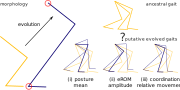
\includegraphics[width=16cm]{./figures/Transferability_Evolution.pdf}
\caption{\label{fig:transferability}FCAS facilitates transferability of kinematic data. A hypothetical, non-isometric evolution of morphology must be compensated by changes in (i) posture, (ii) effective range of motion, and (iii) coordination. By separating these effects in kinematic measurements, evolutionary hypotheses can be tested, and the transfer of coordination patterns from one species to another is improved.}
\end{figure}
\end{change}


Explanatory or even predictive considerations require returning to the construct level, and for legged terrestrial locomotion this would be the level of the joints, e.g. measuring the (joint) angles between segments.
Yet there is a standing problem with that construct: joint angles are constrained by morphology, which has been associated with issues of transferability \citep{Gatesy2011}.
This complicates comparison of joint angles between morphologically disparate groups (e.g. between species, or birth weight categories).
For example, \citet{Gatesy2011} assess that motion transfer between a human and flamingo fails\footnote{\textit{Cf.} \url{https://www.youtube.com/watch?v=1Wh8d9b2Wrw}}, causing ``undesirable motion artifacts'' due to morphological discrepancy\footnote{Another popular example for "motion transfer" is the transfer of measured running kinematic data of chicken, \textit{Gallus domesticus}, to animate a \textit{Tyrannosaurus rex}, \textit{cf.} \url{https://www.amnh.org/exhibitions/dinosaurs-ancient-fossils/theropod-biomechanics/walk-dont-run }.}\(^,\)\footnote{These considerations must be flanked by discussions on dynamic similarity \citep{Aerts2023}.}.
They also speculate that underlying patterns of coordination could be invariant to morphological disparity, yet they expose a lack of methods to directly assess coordination.
As shown herein, FCAS enables the isolation of affine components of joint angle profiles, and, by partly removing them, the extraction of measures of coordination.
\chng{I have demonstrated how to generate relative joint angle profiles, which are direct measures of coordination.}
Take a hypothetical lineage which evolves towards elongation \chng{of a single segment} (non-isometric, i.e. the other segments would not elongate similarly; Fig. \ref{fig:transferability}): to retain the ability to walk despite altered morphology, there are three options.
These animals must either (i) change their posture, e.g. by walking with a more extended limb.
In other cases, e.g. an elephant-like, straight limb situation as the ``null'' posture, they must (ii) adjust their effective range of motion to retain locomotor capacity.
Then, (iii) an adjustment of the timing of joint angle changes, i.e. coordination, would follow.
This example re-emphasizes the importance of being able to separate affine components (i, ii) and to process the remaining variables (iii) alone.
The path for future researchers would be to select a suitable phylogenetic branch or example (maybe Tragulidae or Giraffidae, or more broadly Ruminantia), apply FCAS, and measure how a multivariate block of morphological variables correlates to affine and non-affine components of the joint angle data \citep[a suitable method might be Two-Block Partial Least Squares,][]{Rohlf2000}.
FCAS is the door-opener: at first instance, it can help to identify the mismatching aspects which prohibit motion transfer \citep{Gatesy2011}.
It allows for the separation of different logical components of kinematics (especially coordination; Fig. \ref{fig:transferability}), potentially making some of them transferable.
Motion transfer is in fact the extrapolation of kinematic aspects of one species or comparative category to another, i.e. a predictive problem.
The application of a predictive model of NBW kinematics to LBW in this thesis is an implicit form of motion transfer: which age/size would we assign to an NBW which walked like the LBW we observe?
FCAS thus enables predictive modeling at the construct level of locomotion.

\bigskip
The Fourier-method is not always applicable, but often.
Oscillation, i.e. that a limb configuration changes repetitively over time, is a common scheme in all kinds of locomotor patterns: be it a baboon hindlimb flexing-extending-flexing-extending on a bipedal walk to a water hole \citep{Druelle2021}, or be it an ungulate head-nodding in rhythm with its locomotion \citep{Loscher2016}.
There are multiple reasons for the abundance of oscillation in vertebrate locomotion.
The bone-joint system of vertebrates is well approximated by rigid bodies, which can rotate, but hardly translate with respect to each other.
There are other structural constraints, e.g. elastic elements such as the nuchal ligament which has a crucial role in head nodding.
There is neural organization: brain circuits are known to exhibit oscillations as well \citep{Gupta2016}, which might project downstream.
Furthermore, the evolution-like optimization of behavioral tasks: there is little use to gain efficiency in a one-time control unit, yet repeated modules of a task are worth adjustment; this situation might have favored recurrent locomotor modes (but note that those are not omnipresent: think of cephalopod benthic crawling).
In the many cases which show repetitive or recurrent behavior, Fourier analysis is the natural first choice for transformation.
\section{\chng{Methodological Advances}}
\label{sec:orgbada8d3}
\begin{change}
To summarize: the Fourier method presented herein complements existing analysis strategies for locomotor kinematics by transforming the data to the frequency domain.
This enables the isolation of affine components, which quantify the dynamic posture, effective range of motion, and the coordination of segments.
Though these components could in principle be extracted from raw profiles, the transformation yields them directly.
The advantages are the following.
\begin{itemize}
\item The transformation changes the \textbf{data structure}. Fourier coefficients are more accessible to multivariate statistics, such as PCA and statistical modeling (Ch. \ref{cpt:fcas} and \ref{cpt:piglets}).
\item \textbf{Information retention:} FSD conserves information and is reversible, which means that any model interpolations or predictions can be converted back to kinematic data, which enable dynamic simulations (e.g. to test for stability).
\item FCAS enables \textbf{motion transfer within} a sequence of joints: some or all affine components can be transferred to adjacent joints (Ch. \ref{cpt:fcas}), leaving the residual, relative movement, i.e. coordination.
\item The method is \textbf{complementary} with existing analysis strategies: for example, one can revert the ``coordination'' residual of an FCAS to temporal profiles and perform statistical parametric mapping (appendix \ref{cpt:spm1d}).
\item \textbf{Motion transfer among} study groups: because of the separation of affines and the altered data structure, one can study and test evolutionary trajectories (again, via simulation).
\item Fourier Series and its inversion are trivial to apply, they are \textbf{deterministic transformations}, and code is readily available or easy to obtain in any common programming language (Ch. \ref{appendix:code}).
\end{itemize}


These new possibilities come with a major limitation: Fourier Series decomposition demands temporal periodicity.
Joint angle profiles must be cyclic, i.e. end at the angle where they started.
Another limitation is that rather complex profiles might theoretically require a rather high number of coefficients, as do situations with multiple joints and 3D angles (which were not exhaustively explored in this work).

On the other hand, the nature of locomotion is that there are oscillating limb elements which often move in cyclical patterns.
There are non-invasive tricks to achieve cyclicity, some of which I demonstrated herein (e.g. end-start matching, \ref{properties:endstart}).


This connects the first two parts of this thesis to the third one.
It would have been desirable to link Fourier coefficients of piglet kinematics to dynamic simulations of their limb segments.
For example, an immediate question is which segment movements are responsible for which components of joint moments.
Because of the inconclusive attempts to extract inertial properties from CT scans, and because of the reported inaccuracies in markerless motion tracking, I failed to establish such links between kinematics and dynamics (Ch. \ref{cpt:inertials}).
I anticipate that frequency domain considerations hold some unexplored potential in this direction.


Finally, there is some benefit in using probabilistic frameworks when modeling locomotion.
The motor output of biological systems is intrinsically variable, and an animal which is stable on one stride can tumble on the next one.
Working with likelihoods and probabilities of kinematic patterns seems to better reflect the nature of the process.
\end{change}
\section{How and Why Piglets Move}
\label{sec:org72e349c}
The primary goal of this thesis was to falsify the hypothesis that there are differences in locomotion of low- and normal birth weight piglets (LBW and NBW, Ch. \ref{cpt:generalintro}).
There are two main aspects in which the study groups could differ: in kinematics (\emph{how} animal limb segments move) and dynamics (\emph{why} animal limb segments move as observed).
And there are putatively confounding effects: locomotor maturation (i.e. age), size and weight of the animals \citep[i.e. physical appearance, cf.][]{Aerts2023}, and the variability of locomotor behavior.


Previous studies from our group have compared kinematics on the level of spatiotemporal characteristics of newborn piglet gait \citep{VandenHole2018}.
They discussed delayed locomotor maturation as a proximal explanation of the observed difference.
I herein extended their analysis and confirmed maturational delay by training probabilistic models on the FCAS data of a large number of NBW piglet strides, applied to LBW observations (Ch. \ref{cpt:piglets}).
The FCAS data entering the model contains literally all kinematic information which could be used to distinguish the study groups.
The predictive models accurately incorporate the variability of the phenomenon.
The models predict size and weight of the LBW piglets as if they were ``normal'', i.e. there are no apparent kinematic differences which would lead the model to infer non-normal subject characteristics.
The only differences found are related to the age of LBW piglets.
This indicates that, if models would not consider age or maturation as a model factor, low- and normal birth weight piglet locomotion would be indistinguishable.
The ``age'' model provided evidence that maturation of LBW locomotion halts approximately four hours \emph{post partum} (developmental delay).
We suspect competition within litters and limited metabolic reserves as the reason for developmental delay \citep{VandenHole2019}.

Note that these observations are restricted to walking gait at voluntary speed; we cannot exclude more obvious LBW/NBW differences emerging in more challenging motor tasks.
However, the apparent developmental delay in even this basic motor skill indicates the high sensitivity of the method.
Also, the relevance of any hypothetical, ``more challenging'' stair, treadmill, or wind tunnel experiment for animals whose major priority is to find and access their mother's teats is questionable.
Overall, the models provide strong evidence against the existence of fundamental differences in \emph{how} LBW and NBW piglets move: their coordination seems innate.



\begin{figure}[p]
\centering
\includegraphics[width=12cm]{./figures/piglet_xromm_t02_0214.png}
\caption{\label{fig:piglet_xromm}XROMM using Python and Blender, unpublished. Full video (\url{https://ody.sh/fZe3OpgHGN}) and code (\url{https://git.sr.ht/\~falk/foss\_xromm}) are available.}
\end{figure}

In fact, this lack of differences in the collective output of the animals neuromotor system is surprising.
The FCAS data quantifies joint angle profiles - \chng{which} are indifferent to size.
Yet piglets of low- and normal birth weight operate under different body mass constraints: NBW are about twice as heavy as LBW.
To produce the same kinematics, one would think that they must tune their motors differently, like using different gears.
These would be differences in \emph{why} we observe the (indistinguishable) movements.
Different weight implies different physical constraints, size does matter \citep{Aerts2023}.

Yet we encountered conceptual and practical issues in addressing this second big question (i.e. \emph{why} they move as observed).
The first issue is a practical one (Ch. \ref{cpt:inertials}): inertial parameters, which others have extracted from calibrated CT scans, cannot be determined at sufficient accuracy.
Then, again, there is the issue of variability, as evident from the study of kinematics (Ch. \ref{cpt:piglets}):
differences between NBW and LBW (when normalized for size) seem to be lower in magnitude than the effect of maturation, and lower than normal variability of the behavior.
This was actually confirmed by analysis of 3D kinematics (which we did, unpublished): we originally attempted the full experimental procedure for XROMM.
Of course those recordings are variable, but of the 392 recordings we obtained in several recording sessions in summer 2019, not a single one showed locomotion which strictly fulfilled the ``steady state'' criterion and gave single limb forces (hitting the force plate correctly was likely, but not guaranteed, and happened in 189 recordings, 85 of them walking gait).
Not a single stride could be considered ``representative'', because young piglets in our setup literally always tumbled, jumped, sidestepped, stopped shortly after, or interfered with each other, both LBW and NBW.
The XROMM and inverse dynamics procedure is a low through-put method, and it was not possible to \chng{track landmarks on} a sufficient number of strides to assess LBW differences in joint moment orchestration on the background of motor variability.


These issues notwithstanding, I succeeded in porting the XROMM workflow \citep{Brainerd2010} to an alternative software environment (cf. \url{https://git.sr.ht/\~falk/foss\_xromm}, Fig. \ref{fig:piglet_xromm}).
This workflow includes the complete calculation of inverse dynamics, i.e. joint forces and moments can be visualized.
The software conventionally used for XROMM caused issues: due to its large dependency tree and lack of documentation, XMALab (Brown University, USA, \url{https://xromm.org}) was dysfunctional on the Linux operating system for about half a year during the course of this project; Maya AudoDesk is non-free software.
Except for ORS Dragonfly (Object Research Systems, Canada, \url{https://www.theobjects.com}), which was used for CT segmentation but could be replaced by 3D Slicer (Slicer Community, \url{https://www.slicer.org}), all the tools in the adapted workflow are free and open source.
The example animation (\url{https://ody.sh/fZe3OpgHGN}) can be viewed in Blender (The Blender Foundation, \url{https://blender.org}) from any perspective, and replayed at self-chosen speed.
At the current (incomplete) stage of development, we observe segment position glitches when markers enter or leave the focal volume of the biplanar x-ray.
Also, joint forces and moments do not seem to withstand a visual quality check (their direction and magnitude are sometimes questionable, which falls within the error margin of inertial properties).
This might be an interesting, publishable observation, or a ``bug''; ultimately an error in the computational pipeline cannot be excluded.
Worth noting is that others are currently working in similar directions to open up software alternatives to the conventional XROMM workflow \citep{Falkingham2023}.
At any rate, the primary issues remain the workload of the low through-put XROMM procedure, in contrast to the high through-put demand of appropriate statistics, given the variability of locomotion, coupled with the inaccuracy in determination of inertial segment properties.

The few (three, non-steady) strides which I analyzed and visualized with XROMM techniques with considerable efforts are not representative and cannot provide falsifying evidence with regard to birth-weight dependent differences in piglet locomotor dynamics.


This of course does not imply that there can be no studies of few, representative behavioral observations.
It must be emphasized once more that this major limitation of the present study is tied to two things: the fact that subjects are newborns, and the research question posed herein.
The high variability in locomotor behavior is a specific feature of the ``newborn piglet'' model; at later ages, locomotor behavior stabilizes and becomes more recurrent.
Our research question was whether one can falsify diagnostic differences in LBW and NBW piglets, and the answer must account for stochastic variation to exclude co-incidental findings.
In many other situations, there is either no reason to assume that measurement uncertainty and variability in a behavior are considerable, or they would not prohibit general mechanistic conclusions \citep[e.g.][]{Aerts1998,Astley2012,Montuelle2015}.
Single or rare observations of a behavior can be instructive in many regards \citep[e.g.][]{Druelle2020,Scheidt2022,Dawson2011,Schwarz2020}.
Thus, with most other study settings and subjects, mechanistic evaluations of single strides or actions can generate valuable insights into the workings of the vertebrate musculoskeletal system.


To summarize: this project provided evidence that there is little difference in \emph{how} LBW and NBW piglets move.
Though differences in \emph{why} segments move in a particular way are unlikely in the light of this first finding, methodological limitations prohibited definitive conclusions on dynamic differences in the study groups.
\section{Piglets, Baboons, and Humans}
\label{sec:org786de90}
An important premise of this project was that piglets are a valid model species for humans, in terms of locomotion.
This premise demands constant revision.


Piglets have long been suggested as a model species for human newborns \citep{Book1974,Cooper1975,Mayerl2023}, though there might be alternatives \citep{Mellor1986}.
This suggestion is perfectly justified in the fact that it can be ethically problematic to study human newborns, especially on individuals burdened with an impeded or altered development trajectory.
Piglets are social, sedentary, and share similarity in their appearance (hairless, rotund habitus).
Of course, one has to carefully discuss differences and similarities with the model species, and evaluate alternatives.

One aspect which sets piglets apart from other mammalian model organisms is the relatively high frequency of occurrence of IUGR, Intra-Uterine Growth Retardation \citep{Widdowson1971,Wu2006,VanGinneken2022}.
This diagnosis is different from low birth weight \citep{Wootton1983}, i.e. the lowest quantile of weights in a litter.
Then there is also preterm birth: preterm individuals can have a weight which is lower than normal, but appropriate for gestational age.
Preterms can have low weight for gestational age, or even IUGR, thus double or triple the issues.
Finally, there is low vitality \citep{VandenHole2018}, which is a momentary performance measure (locomotion/respiration scoring), likely linked to the other three state variables.
The situation is complex, classification non-trivial, and there is persistent debate on which indicators matter in which situation.


Nevertheless, researchers study newborn piglets, tracing back epidemiological or congenital issues to histological or structural anomalies.
These can be neurological studies: piglets are somewhat similar to humans in the way their cerebral cortex develops \citep[e.g.][]{Lind2007}, they are available for gene editing \citep{Lind2007}, and a lot of research has focused on neural development in piglets and implications for human infants \citep{Conrad2012,Radlowski2014,Leyshon2016,Mudd2017,Dickerson1971,Fanous2020}.
The piglet model has enabled progress with regard to the research of respiratory problems \citep{Williams1974,Spengler2019}, metabolic issues \citep{Mellor1986,MotaRojas2011,VandenHole2019}, mastication and gut (un-)health \citep{Che2010,Cilieborg2011,Sangild2006,DInca2011,VandenHole2021,Mayerl2023b}.

Maybe most importantly for this thesis, muscle and bone histology and function have been studied \citep{VandenHole2018b,Alvarenga2013,Andersen2016,Aerts2023,Magrini2023}.
Results vary, indicating differences in locomotor performance and muscle mass, but failing to associate them with differences in fibre composition or force generating capacity.

Yet, common to all the organ systems under investigation, it must be stated that analogies of human infants and piglets are usually related to homogeneities on the cellular- or tissue level.
Whereas developmental anomalies in gut, lung, and brain tissue can be related to dysfunctions in neonates of both species, characteristic anomalies of muscle tissue are lacking.
Therefore, though it seems tempting to turn to piglets in light of all the prior research, it might be questionable to choose them as a model \emph{for musculoskeletal aspects}, or even for behavioral aspects which rely on that system.


Other characteristics of the piglet prohibit transfer of findings to our own species, with regard to locomotion.
They are rather precocial \citep{Wischner2009,JYoung2023}, and locomotion of newborns matures at a baffling pace \citep{VandenHole2017,VandenHole2018}.
They are unguligrade, quadrupedal, strictly non-arboreal, and it must be assumed that during the approximately 94 million years of evolution that separate us \citep{Timetree2017} their neural and musculoskeletal anatomy and morphology adapted to different locomotor constraints.


To conclude, I must re-emphasize that piglets are an appropriate and inevitable model species with regard to anomalies on various organ systems.
However, there is little reason to expect relevant conclusions about human locomotor development from piglet research: our locomotor systems are fundamentally different.
Additionally, I quantified a lack of differences in locomotion between low- and normal birth weight piglets (Ch. \ref{cpt:piglets}): it must be assumed that motor control in precocial animals is innate and therefore locomotor capacity indistinguishable.
I cannot exclude that the most severe IUGR or preterm conditions can elicit deficits in kinematics, tracing to impeded neural or musculoskeletal development.
Also, metabolic difference are likely, limiting endurance and vitality of LBWs, which I did not quantify.
But even if such differences occur, they cannot be easily extrapolated to humans.


This opens the discussion about alternative model species.
Non-human primates, e.g. baboons, are sufficiently similar to humans in anatomy and habitus, and their usefulness in medical and evolutionary research is widely accepted \citep{Nardone2017,Liang2023,Aerts2023b,Druelle2021,BoulinguezAmbroise2021}.
Their developmental trajectory is less steep than that of piglets (Ch. \ref{cpt:statistics}), but still on a manageable timescale for longitudinal studies \citep{Druelle2017}.
Ethical concerns in using primates might weigh more strongly (for reasons unknown).
Those objections can be partially mitigated for the kind of locomotor research demonstrated herein:
kinematic studies from calibrated videography are non-invasive.
The inaccuracies of inertial measurements (Ch. \ref{cpt:inertials}) justify doubt on the common practice of euthanizing individuals after experiments; one could as well use naturally deceased specimens, model data, or literature data to transfer the measured inertials to new observations (which would also enable longitudinal inverse dynamic studies).
All this of course demands ethical assessment of, amongst more, proportionate radiation dose (especially on young individuals), appropriate experimental circumstances (e.g. habituation requirement), and general welfare \citep{Young2018}.
The main limiting factor for such studies is the availability of non-human primates and their offspring, even more of IUGR-like conditions, which, as is often argued, is one of the benefits of using domestic piglets as a model.

Yet in the light of the present thesis, it seems more worthwhile to strive for appropriate conditions and experimental circumstances to study species which are more closely related to humans.
\section{Conclusion}
\label{sec:org13597f6}
Independent of the choice of model species, this thesis presented a number of advances in developmental or general studies of locomotor behavior.

\bigskip
Conventional studies of kinematics mainly rely on irreversibly derived spatiotemporal variables.

Raw kinematic traces are often qualitatively compared, yet inaccessible for multivariate statistical analysis.
Fourier Analysis methods are known and rarely used, yet a subtle completion made them more accessible for kinematic analysis: equation \eqref{eqn:affines_phase}, which determines the main phase of a signal.
Together with the delay theorem, a cyclic joint angle profile can be ``rolled'' around the stride cycle for precise temporal alignment.
The affine components (mean, amplitude, phase) of the joint angle profiles can be isolated, allowing a Procrustes-like alignment and more relevant quantitative comparison of temporal patterns in joint angle movement.

I have demonstrated the potential of this set of mathematical tricks on a broad data set of ungulates (comparative/descriptive) and on a longitudinal, developmental data set from piglet kinematics (comparative/predictive).


\bigskip
Transforming kinematic data to the frequency domain and extracting affine components opens up countless possibilities for data analysis.

Variability in locomotor output might be considered a nuisance, yet especially in neonates, variability and the progressive reduction of it are arguably a feature of the system.
Variability enables learning and locomotor maturation; even seemingly innate neuromotor control has to pass the ``reality test''.
Being able to quantify and compare this feature is a huge advantage of probabilistic models.
Predictive modeling, in particular, can be implemented to compare groups (as demonstrated), refine model design, support hypothesis building; models can take an evolutionary, comparative, longitudinal or cross-sectional, or exploratory flavor, or many more.
The modeling toolbox chosen herein has proven to be sufficiently adaptable to handle even complex model constructs, which relate subject characteristics (including morphometrics), spatiotemporal variables, and raw kinematics in FCAS form.
The achievement of the author with regard to probabilistic modeling is mainly educational: these methods are popular in other fields, yet I daresay that few biomechanists are fully aware of their potential.
Consequently, all code produced for this thesis is publicly available for others to adapt and replicate.

With all these data types and modeling capabilities at hand, future researchers can fine tune their models to answer highly specific questions about study subjects and their locomotor development.


\bigskip
In contrast to kinematic data analysis and modeling, my contribution to inverse dynamic modeling is less than what I hoped to achieve.

As discussed above, this is due to the discrepancy in data throughput of the inverse dynamic workflow, and variability of the phenomenon of interest.
Also, initial technical misconceptions about CT scans (Ch. \ref{cpt:inertials}) have temporarily misled my efforts; there were visible problems in the outcome of my custom-made inverse dynamics workflow.
In reaction, the ``flying femur'' experiment as a reductive approach enabled the understanding of all details of the workflow.
This included a sensitivity analysis, which reveals surprisingly high error margins for the inertial properties, which might be prohibitive for inverse dynamic calculations.
I take this as a clear reminder that for anything we measure, we should put all necessary efforts into understanding the mechanistic fundamentals of our measurement, and we must keep track of measurement uncertainty.

Both the reductive approach and the sensitivity analysis are advisable strategies hopefully adopted by future biomechanists.

\bigskip
It is my sincere hope that other researchers take these analysis tools, reproduce, adapt, and correct them where needed, and improve our understanding of how and why various animals move in different phases and circumstances of their existence.
I hope this goal explains some extensive, tutorial-like chapters within this thesis, and it hopefully excuses the colloquial tone of some paragraphs which might not have been to the intended entertainment or taste of every recipient.
\bigskip


Thank you for your interest in my work!



%\chapter{Acknowledgements}\label{acknowledgements}
%tbd.


\cleartorightpage
\part{Appendix}\label{acknowledgements}


%\addcontentsline{toc}{section}{Bibliography}
\singlespacing
\section{Bibliography}
\renewcommand{\bibname}{}
\makeatletter
\renewcommand{\chapter}{\@gobbletwo}
\makeatother
\bibliographystyle{apalike}
\bibliography{library.bib}
%\printbibliography[heading=bibnumbered, title={References}]{library.bib}

\clearpage
\section{Video Digitization}\label{cpt:digitization}
To perform any kinematic analysis, one has to extract kinematic data.
The standard way to do this has changed dramatically during the course of this PhD project.
Some milestone publications are listed here for the interested reader.
More details can be found in the articles marked as ``review''.
The author was involved in one of the studies \citep{MMielke2020}.

\begin{itemize}
\item analog \citep[e.g.][]{Bernstein1927b}
\item (Review) DLTv \citep{Hedrick2008}
\item Argus \citep{Jackson2016}
\item (Review) Progressive Tracking \citep{MMielke2020}
\item DeepLabCut \citep{Mathis2018,Mathis2020}
\item ThruTracker \citep{Corcoran2021}
\item AniPose \citep{Karashchuk2021}
\item (Review) overview deep learning methods \citep{Cronin2021}
\end{itemize}


\clearpage
\section{List of Abbreviations}\label{abbreviations}
\begin{spacing}{1.5}
\begin{small}
\begin{longtable}{l @{ -- } l}
   BFGS & Broyden, Fletcher, Goldfrab, Shanno (Algorithm)
\\ BMD & Bone Mineral Density
\\ BMI & Body Mass Index
\\ CAD & Computer Aided Design (models)
\\ CC & Coordination Component
\\ \chng{\(\vec{COM}\)} & Center Of Mass
\\ CRP & Continuous Relative Phase
\\ CT & computed tomography
\\ DECT & Dual-Energy CT
\\ DFT & Discrete Fourier Transform
\\ DLC & DeepLabCut (video digitization software)
\\ DOF & Degrees Of Freedom
\\ eROM & effective Range Of Motion
\\ FBP & Filtered Backprojection (CT reconstruction algorithm)
\\ FCAS & Fourier Coefficient Affine Superimposition
\\ FFT & Fast Fourier Transform
\\ FSD & Fourier Series Decomposition
\\ \chng{\(\vec{g}\), g} & \chng{gravitational acceleration or its magnitude}
\\ HDI & Highest probability Density Interval
\\ HDS & High Dutyfactor Stride
\\ HMC & Hamiltonian Monte Carlo
\\ HMPE & high-molecular-weight polyethylene
\\ I & Mass Moment of Inertia
\\ ICA & Independent Component Analysis
\\ ICS & Inertial Coordinate System
\\ iff & if, and only if
\\ LBW & (piglet with) Low Birth Weight
\\ LDS & Low Dutyfactor Stride
\\ LED & Light Emitting Diode
\\ LF & left frontlimb
\\ LH & left hindlimb
\\ LKJ & Lewandowski-Kurowicka-Joe prior distribution
\\ LOO & Leave One Out
\\ MCMC & Markov Chain Monte Carlo
\\ NBW & (piglet with) Normal Birth Weight
\\ NUTS & No U-Turn Sampler
\\ \(O\left(\ldots\right)\) & in the Order of ... (magnitude)
\\ PA6 & Nylon 6 / Polycaprolactam
\\ PC & Polycarbonate
\\ PC, PCi & (\(i^{th}\)) Principal Component
\\ PCA & Principal Component Analysis
\\ PCs & Principal Components (see PCA)
\\ PD & Procrustes Distance
\\ PE & Polyethylene
\\ PEEK & Polyether ether ketone
\\ PP & Polypropylene
\\ PTFE & Polytetrafluoroethylene
\\ PVC & Polyvinylchloride
\\ RF & right frontlimb
\\ RH & right hindlimb
\\ ROM & Range Of Motion
\\ \chng{SPM} & \chng{Statistical Parametric Mapping}
\\ WAIC & Widely Applicable Information Criterium
\\ XROMM & X-ray Reconstruction of Moving Morphology
\end{longtable}
\end{small}

\end{spacing}
\end{document}

%
%
